\documentclass[10pt, twoside]{book}   	% use "amsart" instead of "article" for AMSLaTeX format

\newcommand{\theoremsandsuchchapter}{}

% theorems and such

\ifdefined\theoremsandsuchchapter
\newtheorem{definition}{Definition}[chapter]
\newtheorem{theorem}{Theorem}[chapter]
\newtheorem{lemma}{Lemma}[chapter]
\newtheorem{corollary}{Corollary}[chapter]
\newtheorem{conjecture}{Conjecture}[chapter]
\else
\newtheorem{definition}{Definition}
\newtheorem{theorem}{Theorem}
\newtheorem{lemma}{Lemma}
\newtheorem{corollary}{Corollary}
\newtheorem{conjecture}{Conjecture}
\fi

\newcommand{\definename}{Definition}
\newcommand{\theoremname}{Theorem}
\newcommand{\lemmaname}{Lemma}
\newcommand{\corollaryname}{Corollary}

\newenvironment{proof}{\begin{quote}\textit{Proof}:}{\end{quote}}
\newenvironment{solution}{\begin{quote}\textit{Solution}:}{\end{quote}}
\newenvironment{pcode}{\begin{quote}\textit{Python source code}:}{\end{quote}}
\newenvironment{names}{\begin{itshape}}{\end{itshape}}

\newcommand{\qed}{{\bf Q.E.D.}}
\renewcommand{\qed}{\rule[-.5ex]{.5em}{2ex}}
\newcommand{\textfn}[1]{\textsl{#1}}

% table

\newcommand{\tparbox}[2]{%
{\parbox[c]{#1}{\center\vspace{-.4\baselineskip}{#2}\vspace{.3\baselineskip}}}}

% smile
\renewcommand{\smile}{\ensuremath{^\wedge\&^\wedge}}

% softwares

\newenvironment{code}{\begin{quote}\begin{tt}}{\end{tt}\end{quote}}


% math


\newcommand{\bmyeq}{\[}
\newcommand{\emyeq}{\]}
\newcommand{\bmyeql}[1]{\begin{equation}\label{#1}}
\newcommand{\emyeql}{\end{equation}}
%\newenvironment{myeq}{\[}{\]}
%\newenvironment{myeql}[1]{\begin{equation}\label{#1}}{\end{equation}}

\newcommand{\onehalf}{\ensuremath{\frac{1}{2}}}
\newcommand{\onethird}{\ensuremath{\frac{1}{3}}}
\newcommand{\onefourth}{\frac{1}{4}}
\newcommand{\sumft}[2]{\sum_{#1}^{#2}}
\newcommand{\sumioneton}{\sumionetok{n}}
\newcommand{\sumionetok}[1]{\sum_{i=1}^#1}
\newcommand{\sumoneto}[2]{\sum_{#1=1}^{#2}}
\newcommand{\sumoneton}[1]{\sumoneto{#1}{n}}
\newcommand{\prodoneto}[2]{\prod_{#1=1}^{#2}}
\newcommand{\prodoneton}[1]{\prodoneto{#1}{n}}

\newcommand{\listoneto}[1]{\ensuremath{1,2,\ldots,#1}}
\newcommand{\diagxoneto}[2]{\ensuremath{\diag({#1}_1,{#1}_2,\ldots,{#1}_{#2})}}
\newcommand{\setxoneto}[2]{\ensuremath{\{\listxoneto{#1}{#2}\}}}
\newcommand{\listxoneto}[2]{\ensuremath{{#1}_1,{#1}_2,\ldots,{#1}_{#2}}}
\newcommand{\setoneto}[1]{\ensuremath{\{1,2,\ldots,#1\}}}

\newcommand{\diagmat}[2]{\diagoneto{#1}{#2}}

\newcommand{\setoneton}[1]{\setoneton{#1}}
\newcommand{\setxtok}[2]{\setxoneto{#1}{#2}}



\newcommand{\colvectwo}[2]{\ensuremath{\begin{my-matrix}{c}{#1}\\{#2}\end{my-matrix}}}
\newcommand{\colvecthree}[3]{\ensuremath{\begin{my-matrix}{c}{#1}\\{#2}\\{#3}\end{my-matrix}}}
\newcommand{\colvecfour}[4]{\ensuremath{\begin{my-matrix}{c}{#1}\\{#2}\\{#3}\\{#4}\end{my-matrix}}}
\newcommand{\rowvectwo}[2]{\ensuremath{\begin{my-matrix}{cc}{#1}&{#2}\end{my-matrix}}}
\newcommand{\rowvecthree}[3]{\ensuremath{\begin{my-matrix}{ccc}{#1}&{#2}&{#3}\end{my-matrix}}}
\newcommand{\rowvecfour}[4]{\ensuremath{\begin{my-matrix}{cccc}{#1}&{#2}&{#3}&{#4}\end{my-matrix}}}
\newcommand{\diagtwo}[2]{\ensuremath{\begin{my-matrix}{cc}{#1}&0\\0& {#2}\end{my-matrix}}}
\newcommand{\mattwotwo}[4]{\ensuremath{\begin{my-matrix}{cc}{#1}&{#2}\\{#3}&{#4}\end{my-matrix}}}
\newcommand{\bigmat}[9]{\ensuremath{\begin{my-matrix}{cccc} #1&#2&\cdots&#3\\ #4&#5&\cdots&#6\\ \vdots&\vdots&\ddots&\vdots\\ #7&#8&\cdots&#9 \end{my-matrix}}}
%\newcommand{\matdotff}[9]{\matff{#1}{#2}{\cdots}{#3}{#4}{#5}{\cdots}{#6}{\vdots}{\vdots}{\ddots}{\vdots}{#7}{#8}{\cdots}{#9}}

\newcommand{\matthreethree}[9]{%
	\begin{my-matrix}{ccc}%
	{#1}&{#2}&{#3}%
	\\{#4}&{#5}&{#6}%
	\\{#7}&{#8}&{#9}%
	\end{my-matrix}%
}
\newcommand{\matthreethreeT}[9]{%
	\matthreethree%
	{#1}{#4}{#7}%
	{#2}{#5}{#8}%
	{#3}{#6}{#9}%
}

\newenvironment{my-matrix}{\left[\begin{array}}{\end{array}\right]}

\newcommand{\mbyn}[2]{\ensuremath{#1\times #2}}
\newcommand{\realmat}[2]{\ensuremath{\reals^{\mbyn{#1}{#2}}}}
\newcommand{\realsqmat}[1]{\ensuremath{\reals^{\mbyn{#1}{#1}}}}
\newcommand{\defequal}{\triangleq}

\newcommand{\dspace}{\,}
\newcommand{\dx}{{\dspace dx}}
\newcommand{\dy}{{\dspace dy}}
\newcommand{\dt}{{\dspace dt}}
\newcommand{\intspace}{\!\!}
\newcommand{\sqrtspace}{\,}
\newcommand{\aftersqrtspace}{\sqrtspace}
\newcommand{\dividespace}{\!}

\newcommand{\one}{\mathbf{1}}
\newcommand{\arginf}{\mathop{\mathrm{arginf}}}
\newcommand{\argsup}{\mathop{\mathrm {argsup}}}
\newcommand{\argmin}{\mathop{\mathrm {argmin}}}
\newcommand{\argmax}{\mathop{\mathrm {argmax}}}

\newcommand{\reals}{{\mbox{\bf R}}}
\newcommand{\preals}{{\reals_+}}
\newcommand{\ppreals}{{\reals_{++}}}
\newcommand{\complexes}{{\mbox{\bf C}}}
\newcommand{\integers}{{\mbox{\bf Z}}}
\newcommand{\naturals}{{\mbox{\bf N}}}
\newcommand{\rationals}{{\mbox{\bf Q}}}

\newcommand{\realspace}[2]{\reals^{#1\times #2}}
\newcommand{\compspace}[2]{\complexes^{#1\times #2}}

\newcommand{\identity}{\mbox{\bf I}}
\newcommand{\nullspace}{{\mathcal N}}
\newcommand{\range}{{\mathcal R}}

\newcommand{\set}[2]{\{#1~|~#2\}}
\newcommand{\bigset}[2]{\left\{#1\left|#2\right.\right\}}


% operators

\newcommand{\Expect}{\mathop{\bf E{}}}
\newcommand{\Var}{\mathop{\bf  Var{}}}
\newcommand{\Cov}{\mathop{\bf Cov}}
\newcommand{\Prob}{\mathop{\bf Prob}}



% operators

\newcommand{\smallo}{{\mathop{\bf o}}}

\newcommand{\jac}{{\mathcal{J}}}
\newcommand{\diag}{\mathop{\bf diag}}
\newcommand{\Rank}{\mathop{\bf Rank}}
\newcommand{\rank}{\mathop{\bf rank}}
\newcommand{\dimn}{\mathop{\bf dim}}
\newcommand{\Tr}{\mathop{\bf Tr}} % trance
\newcommand{\dom}{\mathop{\bf dom}}
\newcommand{\Det}{\det}
\newcommand{\adj}{\mathop{\bf adj}}
%\newcommand{\Det}{{\mathop{\bf Det}}}
%\newcommand{\determinant}[1]{|#1|}
\newcommand{\sign}{{\mathop{\bf sign}}}
\newcommand{\dist}{{\mathop{\bf dist}}}




% probability space

\newcommand{\probsubset}{{\mathcal{P}}}
\newcommand{\eset}{{\mathcal{E}}}

\newcommand{\probspace}{{\Omega}}


% acronyms

\newcommand{\eg}{{\it e.g.}}
\newcommand{\ie}{{\it i.e.}}
\newcommand{\etc}{{\it etc.}}
\newcommand{\cf}{{\it cf.}}


% some commands & environments for making lecture notes

\newcounter{oursection}
\newcommand{\oursection}[1]{
 \addtocounter{oursection}{1}
 \setcounter{equation}{0}
 \clearpage \begin{center} {\Huge\bfseries #1} \end{center}
 {\vspace*{0.15cm} \hrule height.3mm} \bigskip
 \addcontentsline{toc}{section}{#1}
}
\newcommand{\oursectionf}[1]{  % for use with foiltex
 \addtocounter{oursection}{1}
 \setcounter{equation}{0}
 \foilhead[-.5cm]{#1 \vspace*{0.8cm} \hrule height.3mm }
 \LogoOn
}
\newcommand{\oursectionfl}[1]{  % for use with foiltex landscape
 \addtocounter{oursection}{1}
 \setcounter{equation}{0}
 \foilhead[-1.0cm]{#1}
 \LogoOn
}

\newcounter{lecture}
\newcommand{\lecture}[1]{
 \addtocounter{lecture}{1}
 \setcounter{equation}{0}
 \setcounter{page}{1}
 \renewcommand{\theequation}{\arabic{equation}}
 \renewcommand{\thepage}{\arabic{lecture} -- \arabic{page}}
 \raggedright \sffamily \LARGE
 \cleardoublepage\begin{center}
 {\Huge\bfseries Lecture \arabic{lecture} \bigskip \\ #1}\end{center}
 {\vspace*{0.15cm} \hrule height.3mm} \bigskip
 \addcontentsline{toc}{chapter}{\protect\numberline{\arabic{lecture}}{#1}}
 \pagestyle{myheadings}
 \markboth{Lecture \arabic{lecture}}{#1}
}
\newcommand{\lecturef}[1]{
 \addtocounter{lecture}{1}
 \setcounter{equation}{0}
 \setcounter{page}{1}
 \renewcommand{\theequation}{\arabic{equation}}
 \renewcommand{\thepage}{\arabic{lecture}--\arabic{page}}
 \parindent 0pt
 \MyLogo{#1}
 \rightfooter{\thepage}
 \leftheader{}
 \rightheader{}
 \LogoOff
 \begin{center}
 {\large\bfseries Lecture \arabic{lecture} \bigskip \\ #1}
 \end{center}
 {\vspace*{0.8cm} \hrule height.3mm}
 \bigskip
}
\newcommand{\lecturefl}[1]{   % use with foiltex landscape
 \addtocounter{lecture}{1}
 \setcounter{equation}{0}
 \setcounter{page}{1}
 \renewcommand{\theequation}{\arabic{equation}}
 \renewcommand{\thepage}{\arabic{lecture}--\arabic{page}}
 \addtolength{\topmargin}{-1.5cm}
 \raggedright
 \parindent 0pt
 \rightfooter{\thepage}
 \leftheader{}
 \rightheader{}
 \LogoOff
 \begin{center}
 {\Large \bfseries Lecture \arabic{lecture} \\*[\bigskipamount] {#1}}
 \end{center}
 \MyLogo{#1}
}



\usepackage{appendix}
\usepackage{geometry}                		% See geometry.pdf to learn the layout options. There are lots.
\geometry{letterpaper}                   		% ... or a4paper or a5paper or ...
%\geometry{landscape}                		% Activate for rotated page geometry
\usepackage[parfill]{parskip}    		% Activate to begin paragraphs with an empty line rather than an indent
\usepackage{graphicx}				% Use pdf, png, jpg, or eps§ with pdflatex; use eps in DVI mode
								% TeX will automatically convert eps --> pdf in pdflatex
\usepackage{amssymb}
\usepackage{mathtools}

\usepackage{hyperref}
\hypersetup{
    colorlinks=true,
    linkcolor=blue,
    filecolor=magenta,
    %urlcolor=cyan,
    urlcolor=blue,
}

\usepackage{amsmath}

%SetFonts

%SetFonts

\newcommand{\feasibleset}{\mathcal{F}}
\newcommand{\optsolset}{\mathcal{X}^\ast}
\newcommand{\grad}{\nabla}
\newcommand{\possemidefset}[1]{\mathcal{S}_+^{#1}}
\newcommand{\posdefset}[1]{\mathcal{S}_{++}^{#1}}
\newcommand{\covmat}[1]{{\Sigma}_{#1}}


% statistics commands

%\newcommand{\prob}[1]{\Prob\{#1\}}
%\newcommand{\condprob}[2]{\Prob\set{#1}{#2}}
\newcommand{\prob}[1]{P(#1)}
\newcommand{\condprob}[2]{P(#1|#2)}


\title{Mathematics, Statistics, Optimization, and Machine Learning}
\author{Sunghee Yun}
%\date{}							% Activate to display a given date or no date


%\includeonly{app-amazon-mlu}
%\includeonly{part-statistics}
%\includeonly{chp-rl}

\begin{document}

\maketitle

\setcounter{secnumdepth}{4}
\setcounter{tocdepth}{3}
\tableofcontents

%\newpage

\part{Mathematics}

\chapter{Calculus}

\section{Basics}

\begin{theorem}
[L'H\^opital's rule]
Let $f:\reals\to\reals$ and $f:\reals\to\reals$ be differentiable on an open interval $I\subseteq \reals$
except possibly at $c\in I$.
If $\lim_{x\to c} f(x) = \lim_{x\to c} g(x) = 0$ or $\pm \infty$,
$g'(x)=0$ for all $x\in I\backslash \{c\}$,
and $\lim_{x\to c} \frac{f'(x)}{g'(x)}$ exists,
then
\begin{equation}
\label{eq:lhopital-rule}
\lim_{x\to c} \frac{f(x)}{g(x)}
= \lim_{x\to c} \frac{f'(x)}{g'(x)}.
\end{equation}
\end{theorem}

\begin{definition}
[Taylor polynomial]
Let $n\in\integers$ be a positive integer and
let $f:\reals\to\reals$ be $n$ times differentiable at $a\in\reals$.
The $n$-th order Taylor polynomial is defined by
\begin{eqnarray}
T_{f,n}(x) &=& f(a) + f'(a)(x-a)
+ \frac{f''(a)}{2!}(x-a)^2
+ \cdots
+ \frac{f^{(n)}(a)}{n!}(x-a)^n
\nonumber
\\
&=&
\sum_{k=0}^n \frac{f^{(k)}(a)}{k!} (x-a)^k
\label{eq:taylor-poly}
\end{eqnarray}
\end{definition}


\begin{theorem}
[Taylor's theorem]
\label{theorem:taylor-peano}
Let $n\in\integers$ be a positive integer and
let $f:\reals\to\reals$ be $n$ times differentiable at $a\in\reals$.
Then there exists a function $h_n:\reals\to\reals$ such that
\begin{equation}
\label{eq:taylor-peano}
f(x) = T_{f,n}(x) + h_n(x) (x-a)^n
\end{equation}
and $\lim_{x\to a} h_n(x)=0$.
The remainder is called the Peano form of the remainder.
\end{theorem}

\begin{theorem}
[Taylor's theorem]
\label{theorem:taylor-lagrange}
Let $n\in\integers$ be a positive integer, $a,b\in\reals$,
and $I_o = (a,b) \cup (b,a)$ and $I_c = [a,b] \cup [b,a]$.
Let $f:\reals\to\reals$ be $n+1$ times differentiable on $I_o$
and $f^{(n)}$ is continuous on $I_c$.
Then for some $c \in I_o$,
\begin{equation}
\label{eq:taylor-lagrange}
f(b) = T_{f,n}(b) + \frac{f^{(n+1)}(c)}{(n+1)!}(b-a)^{n+1}.
\end{equation}
The remainder is called the Peano form of the remainder.
\end{theorem}


\section{Multivariate functions}

\begin{definition}[Jacobian matrix]
Let $f:\reals^n \to \reals^m$ be a differentiable function,
\ie, the partial derivative $\partial f_j(x) / \partial x_i$ exists for every $1\leq i\leq n$ and $1\leq j\leq m$.
Then the Jacobian matrix of $f$ at $x$ is defined by the function $D_f:\reals^{n} \to \reals^{m \times n}$
such that
\begin{equation}
\label{eq:jacobian-matrix}
D_f(x) = \begin{my-matrix}{cccc}
\partial f_1(x) / \partial x_1
& \partial f_1(x) / \partial x_2
& \cdots
& \partial f_1(x) / \partial x_n
\\
\partial f_2(x) / \partial x_1
& \partial f_2(x) / \partial x_2
& \cdots
& \partial f_2(x) / \partial x_n
\\
\vdots & \vdots & \ddots & \vdots
\\
\partial f_m(x) / \partial x_1
& \partial f_m(x) / \partial x_2
& \cdots
& \partial f_m(x) / \partial x_n
\end{my-matrix}
\in\reals^{m \times n}.
\end{equation}
\end{definition}



\section{Chain rule}

\begin{theorem}
\label{theorem:chain-rule}
Let $f:\reals\to\reals^n$ and $g:\reals^n\to\reals$ be differentiable.
Then $h:\reals\to\reals$ such that $h(t) = g(f(t))$ is also differentiable and
\[
h'(t) = \sum_{i=1}^n f_i'(t) \frac{\partial g}{\partial x_i} (f(t))
= \nabla^T g(f(t))^T D_f (t)
\]
for all $t\in\dom f$.
\end{theorem}

\begin{corollary}
\label{corollary:chain-rule-gen}
Let $f:\reals^n\to\reals^m$ and $g:\reals^m\to\reals^p$ be differentiable.
Then define a function $h:\reals^n\to\reals^p$ such that $h(x) = g(f(x))$ for all $x\in\dom f$.
Then $h$ is differentiable and
\begin{equation}
\label{eq:chain-rule-gen}
D h(x) = Dg(f(x)) Df(x)
\end{equation}
where
$D f:\reals^n\to\reals^{m\times n}$,
$D g:\reals^m\to\reals^{p\times m}$,
and $D f:\reals^n\to\reals^{p\times n}$
are the Jacobian matrix functions of $f$, $g$, and $h$ respectively.
\end{corollary}

\begin{corollary}
\label{corollary:dixu}
Let $f:\reals^n\to\reals$ be differentiable.
Then for some $A\in\reals^{n\times m}$ and $b\in\reals^n$,
define $g:\reals^m\to\reals$ such that $g(y) = f(Ay+b)$.
Then
\begin{equation}
\label{eq:dixu}
\nabla g(y) = A^T \nabla f(Ay+b).
\end{equation}
\end{corollary}


\begin{corollary}
\label{corollary:eicg}
Let $f:\reals^n\to\reals$ be twice differentiable.
Then for some $A\in\reals^{n\times m}$ and $b\in\reals^n$,
define $g:\reals^m\to\reals$ such that $g(y) = f(Ay+b)$.
Then
\begin{equation}
\label{eq:eicg}
\nabla^2 g(y) = A^T \nabla^2 f(Ay+b)A.
\end{equation}
\end{corollary}

\section{Integration}


\begin{lemma}
Let $A\in\reals^{n\times n}$ be a nonsingular matrix. Suppose that the following integral exists for some $C\subseteq \reals^n$.
\begin{equation}
\int_{C} f(x) dx
\end{equation}
\end{lemma}





\chapter{Convex analysis}

\section{Convex function}

A function $f:\reals^n\to\reals$ is a convex function if, for all $x,y \in \dom f$ and all $0\leq \lambda \leq 1$,
\begin{equation}
f(\lambda x + (1-\lambda)y)
\leq
\lambda f(x) + (1-\lambda)f(y).
\end{equation}

\begin{theorem}
\label{theorem:cvx-equiv-1d-fcn}
Let $f:\reals^n\to\reals$.
Then for some $x\in\dom f$ and $v\in\reals^n$,
define a function $g_{x,v}(t):\reals\to\reals$ such that $g_{x,v}(t) = f(x+tv)$
with the domain, $\set{t\in\reals}{x+tv\in \dom f}$.
Then $f$ is a convex function iff $g_{x,v}$ is a convex function for any $x\in\dom f$ and any $v\in\reals^n$.
\end{theorem}

\begin{proof}
Suppose that $f$ is a convex function.
Then for any $x\in\dom f$ and $v\in\reals^n$,
for any $s,t \in\set{t\in\reals}{x+tv\in \dom f}$ and any $\lambda\in\reals$ such that $0\leq \lambda \leq 1$,
\begin{eqnarray*}
\lefteqn{
g_{x,v}(\lambda s + (1-\lambda) t)
=f(x+(\lambda s + (1-\lambda) t)v)
}
\\
&=&
f(\lambda (x+sv) + (1-\lambda) (x+tv))
\\
&\leq&
\lambda f(x+sv) + (1-\lambda) f(x+tv)
= \lambda g_{x,v}(s) + (1-\lambda) g_{x,v}(t).
\end{eqnarray*}
Therefore $g_{x,v}$ is a convex function.

Now assume that
$g_{x,v}(t):\reals\to\reals$ is a convex function for any $x\in\dom f$ and $v\in\reals^n$.
Then for any $x,y \in \dom f$ and any $\lambda\in\reals$ such that $0\leq \lambda \leq 1$,
\begin{eqnarray*}
\lefteqn{
f((1-\lambda) x + \lambda y ) =f(x + \lambda (y-x) )
}
\\
&=&
g_{x,y-x}(\lambda)
= g_{x,y-x}((1-\lambda)\cdot 0 + \lambda \cdot 1)
\leq (1-\lambda) g_{x,y-x}(0) + \lambda g_{x,y-x}(1)
\\
&=&
(1-\lambda) f(x) + \lambda f(y),
\end{eqnarray*}
thus, $f$ is a convex function.
\end{proof}

\subsection{First order condition}

\begin{theorem}
\label{theorem:cvx-1st-order-cond-1}
If a function $f:\reals\to\reals$ is differentiable, it is a convex function iff, for all $x, y \in \dom f$,
\begin{equation}
\label{eq:cvx-1st-order-cond-1}
        f(y) \geq f(x) + f'(x) (y-x).
\end{equation}
\end{theorem}

\begin{proof}
Suppose that $f$ is a convex function.
Then assume that $y>x$. Let $h\in\reals$ be a positive number such that $h<y-x$. Then the definition of convexity implies that
\[
f(x+h) \leq (1-\lambda) f(x) + \lambda f(y)
\]
where $\lambda = h/(y-x)$ since
\[
(1-\lambda) x + \lambda y = x + \lambda (y-x) = x +h.
\]
Thus
\[
f(x+h) - f (x) \leq \lambda (f(y)-f(x)) = \frac{h}{y-x} (f(y)-f(x)),
\]
which implies
\[
f'(x) = \lim_{h\to0} \frac{f(x+h) - f (x)}{h} \leq \frac{f(y)-f(x)}{y-x}.
\]
Therefore
\[
f(y) - f(x) \geq f'(x)(y-x),
\]
hence (\ref{eq:cvx-1st-order-cond-1}) is true when $y>x$.

We can prove (\ref{eq:cvx-1st-order-cond-1}) is true when $y<x$ using the very same method.
Assume that $x>y$. Let $h\in\reals$ be a positive number such that $h<x-y$. Then the definition of convexity implies that
\[
f(x-h) \leq (1-\lambda) f(x) + \lambda f(y)
\]
where $\lambda = h/(x-y)$ since
\[
(1-\lambda) x + \lambda y = x + \lambda (y-x) = x -h.
\]
Thus
\[
f(x) - f (x-h) \geq \lambda (f(x)-f(y)) = \frac{h}{x-y} (f(x)-f(y)),
\]
which implies
\[
f'(x) = \lim_{h\to0} \frac{f(x) - f (x-h)}{h} \geq \frac{f(x)-f(y)}{x-y}  =\frac{f(y)-f(x)}{y-x}.
\]
Therefore
\[
f(y) - f(x) \geq f'(x)(y-x),
\]
hence (\ref{eq:cvx-1st-order-cond-1}) is true when $y<x$.
It is obvise that (\ref{eq:cvx-1st-order-cond-1}) is true when $y=x$.
Hence we have just proved that if $f:\reals\to\reals$ is a convex function, then (\ref{eq:cvx-1st-order-cond-1}) holds
for any $x,y\in\dom f$.

Now we prove the converse.
Suppose that (\ref{eq:cvx-1st-order-cond-1}) holds for any $x,y\in\dom f$.
Now let $x,y\in\dom f$ and $\lambda \in \reals$ suc that $0\leq \lambda \leq 1$.
Let $z=\lambda x + (1-\lambda) y$. Then (\ref{eq:cvx-1st-order-cond-1}) implies that
\begin{equation}
\label{eq:dkfj-1}
f(x) - f(z) \geq f'(z) (x-z) = (1-\lambda) f'(z) (x-y)
\end{equation}
and
\begin{equation}
\label{eq:dkfj-2}
f(y) - f(z) \geq f'(z) (y-z) = \lambda f'(z) (y-x)
\end{equation}
If we multiply $\lambda$ on both sides of (\ref{eq:dkfj-1}),
multiply $1-\lambda$ on both sides of (\ref{eq:dkfj-2}),
and add both sides, we have
\[
\lambda(f(x) - f(z)) + (1-\lambda) (f(y) - f(z))
\geq \lambda f(x) +(1-\lambda) f(y) - f(z) \geq 0,
\]
hence
\[
f(\lambda x + (1-\lambda) y)
\leq \lambda f(x) + (1-\lambda) f(y).
\]
Therefore $f$ is a convex function.
\end{proof}

\begin{corollary}
\label{corollary:cvx-deriv-non-decreasing}
Let $f:\reals\to\reals$ be differentiable. Then $f$ is a convex function iff the derivative of $f$ is a nondecreasing function.
\end{corollary}
\begin{proof}
Suppose that $f$ is a convex function.
Let $x,y\in\dom f$ such that $x<y$.
Then \theoremname~\ref{theorem:cvx-1st-order-cond-1} implies
\[
f(y) \geq f(x) + f'(x)(y-x)
\]
and
\[
f(x) \geq f(y) + f'(y)(x-y),
\]
thus
\[
f'(x) \leq \frac{f(y)-f(x)}{y-x}
= \frac{f(x)-f(y)}{x-y} \leq f'(y)
\]
since $y>x$.
Therefore $f'$ is a nondecreasing function.

Now we prove the converse. Suppose that $f'$ is a nondecreasing function.
Then if $y>x$, the mean value theorem implies that there exists some $z \in (x,y)$ such that
\[
\frac{f(y)-f(x)}{y-x} = f'(z).
\]
Since $f'$ is nondecreasing, we have
\[
f'(x) \leq \frac{f(y)-f(x)}{y-x} \leq f'(y),
\]
thus
\begin{equation}
\label{eq:cias-1}
f(y) \geq f(x) + f'(x)(y-x)
\end{equation}
and
\begin{equation}
\label{eq:cias-2}
f(y) \leq f(x) + f'(y)(y-x).
\end{equation}
Therefore (\ref{eq:cias-1}) implies that $f$ satisfies (\ref{eq:cvx-1st-order-cond-1}).
Now if $x>y$, (\ref{eq:cias-2}) implies that
\[
f(x) \leq f(y) + f'(x)(x-y)
\Leftrightarrow
f(y) \geq f(x) + f'(x)(y-x)
\]
which again implies that $f$ satisfies (\ref{eq:cvx-1st-order-cond-1}).
Therefore (\ref{theorem:cvx-1st-order-cond-1}) implies that $f$ is a convex function.
\end{proof}

\begin{corollary}
\label{corollary:cvx-1st-order-cond}
If a function $f:\reals^n\to\reals$ is differentiable, it is a convex function iff, for all $x,y \in \dom f$,
\begin{equation}
\label{eq:cvx-1st-order-cond}
        f(y) \geq f(x) + \nabla f(x)^T (y-x).
\end{equation}
\end{corollary}

\begin{proof}
Suppose that $f$ is a convex function.
Let $x,y\in\dom f$.
If we let $g_{x,y-x}:\reals\to\reals$ be a function such that $g_{x,y-x}(t) = f(x+t(y-x))$,
\theoremname~\ref{theorem:cvx-equiv-1d-fcn} implies $g_{x,y-x}$ is a convex function.
Therefore \theoremname~\ref{theorem:cvx-1st-order-cond-1} together with \corollaryname~\ref{corollary:dixu}
implies
\[
f(y) = g_{x,y-x}(1) \geq g_{x,y-x}(0) + g_{x,y-x}'(0) (1-0)
= f(x) + \nabla f(x) ^T (y-x)
\]
for any $x,y \in \dom f$.

Now suppose that (\ref{eq:cvx-1st-order-cond}) holds for any $x,y \in \dom f$.
Then \corollaryname~\ref{corollary:dixu} implies that,
for any $r,s\in\reals$ and $v\in\reals^n$ such that $r,s\in\set{t\in\reals}{x+tv\in\dom f}$,
\[
g_{x,v}(r) = f(x+rv) \geq f(x+sv) + (r-s) \nabla f(x+sv)^T v = g_{x,v}(s) + g_{x,v}'(s)(r-s).
\]
Thus \theoremname~\ref{theorem:cvx-1st-order-cond-1} implies
$g_{x,v}$ is a convex function for any $x\in\dom f$ and $v\in\reals^n$.
Therefore by \theoremname~\ref{theorem:cvx-equiv-1d-fcn}, $f$ is a convex function.
\end{proof}

\subsection{Second order condition}

\begin{theorem}
\label{theorem:cvx-2nd-order-cond-1}
If a function $f:\reals\to\reals$ is twice differentiable, it is a convex function iff, for all $x \in \dom f$,
\begin{equation}
\label{eq:cvx-2nd-order-cond-1}
        f''(x) \geq 0.
\end{equation}
\end{theorem}

\begin{proof}
Suppose that $f$ is a convex function.
Then \corollaryname~\ref{corollary:cvx-deriv-non-decreasing} implies that $f'$ is a nondecreasing function,
hence
\[
f''(x)
= \lim_{h\to0} \frac{f'(x+h) - f'(x)}{h}
= \lim_{h\to0^+} \frac{f'(x+h) - f'(x)}{h} \geq 0.
\]
Now if $f''(x)\geq0$ for all $x\in\dom f$, the mean value theorem implies that $f'$ is a nondecreasing function.
\end{proof}


\begin{theorem}
\label{theorem:cvx-2nd-order-cond}
If a function $f:\reals^n\to\reals$ is twice differentiable, it is a convex function iff, for all $x \in \dom f$,
\begin{equation}
\label{eq:cvx-2nd-order-cond}
        \nabla^2 f(x) \succeq 0.
\end{equation}
\end{theorem}

\begin{proof}
Suppose that $f$ is a convex function.
Then \theoremname~\ref{theorem:cvx-equiv-1d-fcn} implies that
for any $x\in\dom f$ and any $v\in\reals^n$,
the function $g_{x,v}:\reals\to\reals$ such that $g_{x,v}(t) = f(x+tv)$
is a convex function in $\set{t\in\reals}{x+tv \in \dom f}$.
Then \theoremname~\ref{theorem:cvx-2nd-order-cond-1} together with \corollaryname~\ref{corollary:eicg}
implies that
\[
v^T \nabla^2 f(x) v = g_{x,v}''(0) \geq0.
\]
Therefore $\nabla^2 f(x) \succeq 0$ for any $x \in \dom f$.

Now if $\nabla^2 f(x) \succeq 0$ for all $x\in\dom f$,
then
\corollaryname~\ref{corollary:eicg}
implies that
$g_{x,v}''(t) = v^T \nabla^2 f(x+tv) v \geq0$ for any $x \in \dom f$ and any $v\in\reals^n$.
Then \theoremname~\ref{theorem:cvx-2nd-order-cond-1} implies
$g_{x,v}$ is a convex function for any $x \in \dom f$ and any $v\in\reals^n$,
hence by \theoremname~\ref{theorem:cvx-equiv-1d-fcn},
$f$ is a convex function.
\end{proof}



\chapter{Linear Algebra}

\section{Vector space}

Cauchy–Schwarz inequality: for $a,b\in\complexes^n$,
\begin{equation}
|a^H b| \leq \|a\|_2 \|b\|_2.
\end{equation}

The generalized form:
for $f:[0,1] \to \complexes$ and $g:[0,1] \to \complexes$,
\begin{equation}
\left|\int_{0}^1 \overline{f(t)} g(t) \, dt \right|
\leq
\left(\int_0^1 |f(t)|^2 dt \, \right)^{1/2}
\left(\int_0^1 |g(t)|^2 dt \, \right)^{1/2}.
\end{equation}

H\"older's inequality: for $a,b\in\complexes^n$, $p>1$, and $q>1$ such that $1/p+1/q=1$,
\begin{equation}
|a^H b| \leq \|a\|_p \|b\|_q.
\end{equation}

The generalized form:
for $f:[0,1] \to \complexes$, $g:[0,1] \to \complexes$,
$p>1$, and $q>1$ such that $1/p+1/q=1$,
\begin{equation}
\left|\int_{0}^1 \overline{f(t)} g(t) \, dt \right|
\leq
\left(\int_0^1 |f(t)|^p dt \, \right)^{1/p}
\left(\int_0^1 |g(t)|^q dt \, \right)^{1/q}.
\end{equation}

When $b=\ones$, the Cauchy-Schwarz inequality implies
\begin{equation}
\|a\|_1 \leq n \|a\|_2
\end{equation}



\section{Eigenvalues}

\subsection{Basic definitions}

Given a square matrix $A\in\reals^{n\times n}$,
if there exist $\lambda \in \complexes$ and nonzero $v \in \complexes^n$ such that
\begin{equation}
        A v = \lambda v
\end{equation}
then $\lambda$ is called an eigenvalue of $A$ and $v$ is called an eigenvector associated with $\lambda$.

If there exist $n$ linearly independent eigenvectors, we have
\begin{equation}
A \begin{my-matrix}{ccc} v_1 & \cdots & v_n \end{my-matrix}
= \begin{my-matrix}{ccc} v_1 & \cdots & v_n \end{my-matrix} \diag(\lambda_1,\ldots,\lambda_n)
\end{equation}
or
\begin{equation}
\label{eq:v8dy}
A V = V \Lambda
\end{equation}
where
\begin{equation}
V = \begin{my-matrix}{ccc} v_1 & \cdots & v_n \end{my-matrix}
\in\complexes^{n\times n}
\end{equation}
and
\begin{equation}
\Lambda = \diag(\lambda_1,\ldots,\lambda_n)
= \begin{my-matrix}{cccc}
\lambda_1 & 0 & \cdots & 0
\\
0 & \lambda_2 & \cdots & 0
\\
\vdots & \vdots & \ddots & \vdots
\\
0 & 0 & \cdots & \lambda_n
\end{my-matrix}
\in\complexes^{n\times n}.
\end{equation}
In this case, $A$ is said to be diagonalizable.

Since $V$ is nonsingular, \ie, invertible, we can rewrite (\ref{eq:v8dy}) as
\begin{equation}
\label{eq:2}
A = V \Lambda V^{-1} \Leftrightarrow V^{-1} A V = \Lambda.
\end{equation}


\subsection{Symmetric matrices}

Given a symmetric matrix $A = A^T\in\reals^{n\times n}$,
all the eigenvalues are real and we can choose $n$ real orthonormal eigenvectors,
\ie,
we can find $n$ eigenvectors $v_1, \ldots, v_n\in\reals^n$
associated with $n$ eigenvectors, $\lambda_1, \ldots, \lambda_n \in \reals$
such that
\begin{equation}
    \|v_i\| = 1
\end{equation}
for $i=1,\ldots,n$
and
\begin{equation}
    v_i^T v_j = 0
\end{equation}
for $1\leq i\neq j\leq n$.
Thus, all symmetric matrices are diagonalizable.

Now (\ref{eq:2}) becomes
\begin{equation}
\label{eq:sym-eigen-decomp}
A = V \Lambda V^T \Leftrightarrow V^T A V = \Lambda
\end{equation}
since
\begin{equation}
V^T V = I_n
\end{equation}
where $I_n\in\reals^{n\times n}$ is the indentity matrix.
We can rewrite (\ref{eq:sym-eigen-decomp}) as
\begin{equation}
\label{eq:sym-eigen-decomp-1}
A =
\begin{my-matrix}{ccc} v_1 & \cdots & v_n \end{my-matrix}
\diag(\lambda_1,\ldots,\lambda_n)
\begin{my-matrix}{c} v_1^T \\ \vdots \\ v_n^T \end{my-matrix}
= \sum_{i=1}^n \lambda_i v_i v_i^T.
\end{equation}

\section{Positive definiteness}

\begin{itemize}

\item
A symmetric matrix $A=A^T\in\reals^{n\times n}$ is called positive semidefinite if for all $x\in\reals^n$,
\begin{equation}
x^T A x \geq 0.
\end{equation}

\item
A symmetric matrix $A=A^T\in\reals^{n\times n}$ is called positive definite if for all nonzero $x\in\reals^n$,
\begin{equation}
x^T A x > 0.
\end{equation}

\item The set of all the $n$-by-$n$ positive semidefinite matrices is (sometimes) denoted by $\possemidefset{n}$,
\ie,
\begin{equation}
\possemidefset{n} = \set{A=A^T\in\reals^{n\times n}}{x^T A x \geq 0 \mbox{ for all } x \in \reals^n}.
\end{equation}

\item The set of all the $n$-by-$n$ positive definite matrices is (sometimes) denoted by $\posdefset{n}$,
\ie,
\begin{equation}
\posdefset{n} = \set{A=A^T\in\reals^{n\times n}}{x^T A x > 0 \mbox{ for all nonzero } x \in \reals^n}.
\end{equation}

\item $A=A^T\in\reals^{n\times n}$ is positive semidefinite if and only if all the eigenvalues of $A$ are nonnegative.

\item $A=A^T\in\reals^{n\times n}$ is positive definite if and only if all the eigenvalues of $A$ are positive.

\begin{proof}
For symmetric $A=A^T$, there exist orthgonal $V\in\reals^{n\times n}$ and diagonal $\Lambda\in\reals^{n\times n}$
such that
\[
A = V \Lambda V^T = \sum_{i=1}^n \lambda_i v_i v_i^T,
\]
thus for any $x\in\reals^n$,
\[
x^T A x = x^T \left(\sum_{i=1}^n \lambda_i v_i v_i^T \right) x
= \sum_{i=1}^n \lambda_i x^T v_i v_i^T x
= \sum_{i=1}^n \lambda_i (v_i^T x)^2.
\]
Therefore if all $\lambda_i$ are nonnegative, $x^T A x\geq0$ for any $x\in\reals^n$, hence $A\in\possemidefset{n}$.
Now assume $A\in\possemidefset{n}$, but $\lambda_j < 0$ for some $j\in\{1,\ldots,n\}$.
Then
\begin{equation}
v_j^T A v_j
= \sum_{i=1}^n \lambda_i (v_i^T v_j)^2
= \sum_{i=1}^n \lambda_i \delta_{i,j}
= \lambda_j < 0
\end{equation}
since $v_1$, \ldots, $v_n$ are orthonormal
where
$\delta_{i,j}$ is the \href{https://en.wikipedia.org/wiki/Kronecker_delta}{Kronecker delta function},
hence $A\not \in \possemidefset{n}$.
Therefore if $A\in\possemidefset{n}$, all $\lambda_i$ are nonnegative.

Therefore $A\in\possemidefset{n}$ if and only if all $\lambda_i$ are nonnegative.

Now assume that all $\label_i$ are positive.
Then for all nonzero $x\in\reals^n$,
there exists $i\in\{1,\ldots,n\}$ such tat $v_i^Tx$
since if $v_i^Tx=0$ for all $i$, then
$V^T x = 0$, hence $x=0$ since $V^T$ is nonnsigular.
Therefore
\begin{equation}
x^T A x = \sum_{i=1}^n \lambda_i (v_i^T x)^2
\geq \lambda_j (v_j^T x)^2 > 0.
\end{equation}
Thus, $A\in\posdefset{n}$.

Now assume that $A\in\posdefset{n}$.
If $\lambda_j \leq 0$ for some $j\in\{1,\ldots,n\}$,
then
\begin{equation}
v_j^T A v_j
= \sum_{i=1}^n \lambda_i \delta_{i,j}
= \lambda_j \leq 0,
\end{equation}
hence $A\not\in\posdefset{n}$. Therefore if $A\in\posdefset{n}$, all $\lambda_i$ are positive.

Therefore $A\in\posdefset{n}$ if and only if all $\lambda_i$ are positive.

\end{proof}

\end{itemize}

\section{Matrix norms}

\begin{equation}
\mathbf{dist}( C_\mathrm{org 1}, C_\mathrm{org 2} ) = 
\|C_\mathrm{org 1} - C_\mathrm{org 2} \|
= |\lambda_\mathrm{max}(C_\mathrm{org 1} - C_\mathrm{org 2})|
\end{equation}



\part{Optimization}

\newcommand{\optdomain}{\mathcal{D}}

\section{Mathematical optimization problem}

A mathematical optimization problem can be expressed as
\begin{equation}
\label{eq:opt-prob}
\begin{array}{ll}
\mbox{minimize} & f_0(x)
\\
\mbox{subject to} & f_i(x) \leq 0 \mbox{ for } i = 1, \ldots, m
\\
& h_i(x) = 0 \mbox{ for } i = 1, \ldots, p
\end{array}
\end{equation}
where
$x\in\reals^n$ is the optimization variable,
$f_0:\reals^n\to\reals$ is the objective function,
$f_i:\reals^n\to\reals$ for $i=1,\ldots,n$ are the inequality constraint functions,
and
$h_i:\reals^n\to\reals$ for $i=1,\ldots,p$ are the equality constraint functions.

The conditions, $f_i(x) \leq 0$ for $ i = 1, \ldots, m$, are called inequality constraints
and the conditions, $ h_i(x) = 0 $ for $ i = 1, \ldots, p$ are called equation constraints.

Note that this formulation covers pretty much every single-objective optimization problem.
For example,
consider the following optimization problem.

\begin{equation}
\begin{array}{ll}
\mbox{maximize} & f(x_1,x_2)
\\
\mbox{subject to} & x_1 \geq x_2
\\
& x_1 + x_2 = 2
\end{array}
\end{equation}
This problem can be cast into an equivalent problem as follows.
\begin{equation}
\begin{array}{ll}
\mbox{minimize} & -f(x_1,x_2)
\\
\mbox{subject to} & - x_1 + x_2 \leq 0
\\
& x_1 + x_2 - 2 = 0
\end{array}
\end{equation}


The feasible set for (\ref{eq:opt-prob}) is defined by the set of $x\in\reals^n$ which satisfies all the contraints.
Also, the optimal value for (\ref{eq:opt-prob}) is the infimum of $f_0(x)$ while $x$ is in the feasible set.
When the infimum is achievable, we define the optimal solution set as the set of all feasible $x$ achieving
the infimum value.
These are defined in mathematically rigorous terms below.

\begin{itemize}

\item
The feasible set for (\ref{eq:opt-prob}) is defined by
\begin{equation}
\feasibleset
=
\set{x\in \mathcal{D}}
{ f_i(x)\leq 0 \mbox{ for } i =0, \ldots, m,\ h_j(x) = 0 \mbox{ for } j = 1,\ldots,p}
\subseteq \reals^n
\end{equation}
where
\begin{equation}
\mathcal{D} = \left( \bigcap_{0\leq i\leq m} \dom f_i \right) \cap \left( \bigcap_{1\leq i\leq p} \dom h_i \right).
\end{equation}

\item
The optimal value for (\ref{eq:opt-prob}) is defined by
\begin{equation}
p^\ast = \inf_{x\in\feasibleset} f_0(x)
\end{equation}

We use the conventions that $p^\ast = -\infty$ if $f_0(x)$ is unbounded below for $x\in \feasibleset$
and that $p^\ast = \infty$ if $\feasibleset = \emptyset$.

\item
The optimal solution set for (\ref{eq:opt-prob}) is defined by
\begin{equation}
\optsolset = \set{x\in\feasibleset}{f_0(x) = p^\ast}.
\end{equation}


\end{itemize}


\section{Convex optimization problem}

A mathematical optimization problem is called a convex optimization problem
if the objective function and all the inequality constraint functions are convex functions
and all the equality constraint functions are affine functions.

Hence, a convex optimization problem can be expressed as
\begin{equation}
\label{eq:cvx-opt-prob}
\begin{array}{ll}
\mbox{minimize} & f_0(x)
\\
\mbox{subject to} & f_i(x) \leq 0 \mbox{ for } i = 1, \ldots, m
\\
& A x = b
\end{array}
\end{equation}
where
$x\in\reals^n$ is the optimization variable,
$f_i:\reals^n\to\reals$ for $i=0,\ldots,n$ are convex functions,
$h_i:\reals^n\to\reals$ for $i=1,\ldots,p$ are the equality constraint functions,
$A \in \reals^{p\times n}$, and $b\in\reals^p$.

A function, $f:\reals^n \to \reals$, is called a convex function if
$\dom f \subseteq \reals^n$ is a convex set
and
for all $x, y\in\dom f$
and all $0\leq \lambda \leq 1$,
\begin{equation}
    f( \lambda x + (1-\lambda) y) \leq
    \lambda f(x) + (1-\lambda) f(y)
\end{equation}
where $\dom f \subseteq \reals^n$ denotes the domain of $f$.

A convex optimization enjoys a number of nice theoretical and practical properties.

\begin{itemize}
\item A local minimum of a convex optimization problem is a global minimum,
\ie,
if for some $R>0$ and $x_0\in\feasibleset$, $\|x-x_0\|<R$ and $x\in\feasibleset$ imply $f_0(x_0) \leq f_0(x)$,
then $f_0(x_0) \leq f_0(x)$ for all $x\in\feasibleset$.
\begin{proof}
Assume that $x_0\in\feasibleset$ is a local minimum, \ie,
for some $R>0$, $\|x-x_0\|<R$ and $x\in\feasibleset$ imply $f_0(x_0) \leq f_0(x)$.

Now assume that $x_0$ is not a global minimum, \ie, there exists $y\in\feasibleset$
such that $y\neq x_0$ and $f_0(y) < f_0(x_0)$.
Then for $z = \lambda y + (1-\lambda) x_0$ with $\lambda = \min\{ R/\|y-x_0\|, 1\}/2$,
the convexity of $f_0$ implies
\begin{equation}
\label{eq:4}
f_0(z) \leq \lambda f_0(y) + (1-\lambda) f_0(x_0)
\end{equation}
since $0 < \lambda \leq 1/2 < 1$.
Furthermore
\begin{equation}
\|z - x_0\| = \lambda \|y-x_0\| \leq R/2,
\end{equation}
hence $f_0(z) \geq f_0(x_0)$, which together with (\ref{eq:4}) implies
\begin{equation}
f_0(x_0) \leq f_0(z)
\leq \lambda f_0(y) + (1-\lambda) f_0(x_0)
< \lambda f_0(x_0) + (1-\lambda) f_0(x_0)
= f_0(x_0),
\end{equation}
which is a contradiction.
Therefore there is no $y\in\feasibleset$ such that $y\neq x_0$ and $f_0(y) < f_0(x_0)$.
Therefore $x_0$ is a global minimum.
\end{proof}



\item For a unconstrained problem, \ie, the problem (\ref{eq:cvx-opt-prob}) with $m=p=0$, with differentiable objective function,
$x\in\dom f_0$ is an optimal solution if and only if $\grad f_0(x)= 0 \in \reals^n$.

\begin{proof}
The Taylor theorem implies that for any $x,y\in\dom f_0$,
\begin{equation}
\label{eq:second-order-taylor}
f_0(y) = f(x) + \grad f_0(x) ^T (y-x) + \frac{1}{2} (y-x)^T \grad^2 f_0(z) (y-x)
\end{equation}
for some $z$ on the line segment having $x$ and $y$ as its end points,
\ie, $z = \alpha x + (1-\alpha) y$ for some $0\leq \alpha \leq 1$.
Since $\grad^2 f(x) \succeq0$ for any $z \in \dom f_0$, we have
\begin{equation}
f_0(y) \geq f_0(x) + \grad f_0(x) ^T (y-x)
\end{equation}

Thus, if for some $x_0 \in \reals^n$, $\grad f_0(x_0) = 0$, for any $x\in\dom f_0$,
\begin{equation}
f_0(x) \geq f_0(x_0) + \grad f_0(x_0) ^T (x-x_0) = f_0(x_0),
\end{equation}

hence $x_0$ is an optimal solution.
Now assume that $x_0$ is an optimal solution, but $\grad f_0(x_0) \neq 0$.
Then for any $k>0$, if we let $x=x_0$ and $y = x_0 - k \grad f_0(x_0) $,
(\ref{eq:second-order-taylor}) becomes
\begin{eqnarray*}
\lefteqn{
f_0(y) = f(x_0) + \grad f_0(x_0) ^T (-k \grad f_0(x_0)) + \frac{k^2}{2} \grad f_0(x_0) ^T \grad^2 f_0(z) \grad f_0(x_0)
}
\\
&=&
f(x_0) - k \|\grad f_0(x_0)\|^2 + \frac{k^2}{2} \grad f_0(x_0) ^T \grad^2 f_0(z) \grad f_0(x_0)
\end{eqnarray*}
for all $y = x_0 - k \grad f_0(x_0) \in \dom f_0$.

Since for $k< 2 \|\grad f_0(x_0)\|^2 / \grad f_0(x_0) ^T \grad^2 f_0(z) \grad f_0(x_0)$,
$-k \|\grad f_0(x_0)\|^2 + \frac{k^2}{2} \grad f_0(x_0) ^T \grad^2 f_0(z) \grad f_0(x_0) < 0$,
thus
$f_0(y) < f(x_0)$,
hence the constradiction.
Therefore, if $x_0$ is an optimal solution for the unconstrained problem, $\grad f_0(x_0) = 0$.

\end{proof}
\end{itemize}

\section{Duality}

\subsection{The Lagrange dual problem}

\subsubsection{Examples}

\paragraph{Standard form LP}

\begin{equation}
\begin{array}{ll}
\mbox{minimize} & c^T x
\\
\mbox{subject to} & Ax = b
\\
& x \succeq 0
\end{array}
\end{equation}

The Lagrange dual problem is

\begin{equation}
\begin{array}{ll}
\mbox{maximize} & -b^T \nu
\\
\mbox{subject to} & A^T \nu + c \geq0
\end{array}
\end{equation}

\paragraph{Inequality form LP}

\begin{equation}
\begin{array}{ll}
\mbox{minimize} & c^T x
\\
\mbox{subject to} & Ax \preceq b
\end{array}
\end{equation}

The Lagrange dual problem is

\begin{equation}
\begin{array}{ll}
\mbox{maximize} & -b^T \lambda
\\
\mbox{subject to} & A^T \lambda + c = 0
\\
& \lambda \succeq 0
\end{array}
\end{equation}


\paragraph{Least-squares solution of linear equations}

\begin{equation}
\begin{array}{ll}
\mbox{minimize} & (1/2) x^T x
\\
\mbox{subject to} & Ax = b
\end{array}
\end{equation}

The Lagrange dual problem is

\begin{equation}
\begin{array}{ll}
\mbox{maximize} & -(1/2) \nu^T A A^T \nu - b^T \nu
\end{array}
\end{equation}



\paragraph{Entropy maximization}

\begin{equation}
\begin{array}{ll}
\mbox{minimize} & \sum_{i=1}^n x_i \log x_i
\\
\mbox{subject to} & Ax = b
\\
& \ones^T x = 1
\end{array}
\end{equation}
with domain $\mathcal{D} = \reals^n_+$

The Lagrange dual problem is

\begin{equation}
\begin{array}{ll}
\mbox{maximize} & - b^T \lambda - \log \left( \sum_{i=1}^n \exp(-a_i^T \lambda) \right)
\\
\mbox{subject to} & \lambda  \succeq 0
\end{array}
\end{equation}



\subsection{Interpretations}

\subsubsection{Max-min characterization of weak and strong duality}

We first note that for any $f: X \times Y \to \reals$, we have
\begin{equation}
\sup_{y\in Y} \inf_{x\in X} f(x,y)
\leq \inf_{x\in X} \sup_{y\in Y} f(x,y).
\end{equation}
This inequality is called \emph{max-min inequality}.

We can prove this as follows.
Let $g:Y\to\reals$ be a function defined by $g(y) = \inf_{x \in X} f(x,y)$ and
let $h:X\to\reals$ be a function defined by $h(x) = \sup_{y \in Y} f(x,y)$.
Then we have that for any $x\in X$ and $y\in Y$
\begin{equation}
g(y) = \inf_{x\in X} f(x,y) \leq f(x,y),
\end{equation}
which implies that for any $x\in X$
\begin{equation}
\sup_{y\in Y} g(y) \leq \sup_{y\in Y} f(x,y) = h(x).
\end{equation}
This again implies that
\begin{equation}
\sup_{y\in Y} g(y) \leq \inf_{x\in X} h(x),
\end{equation}
hence the proof.




\subsubsection{Saddle-point interpretation}

Suppose $f:X\times Y \to \reals$.
We refer a point $(\tilde{x}, \tilde{y}) \in X\times Y$ a \emph{saddle-point}
for $f$ (and $X$ and $Y$) if
\begin{equation}
f(\tilde{x},y) \leq f(\tilde{x},\tilde{y}) \leq f(x, \tilde{y})
\end{equation}
for all $x \in X$ and $y\in Y$.

Now if $x^\ast$ and $\lambda^\ast$
are primal and dual optimal points for a problem in which strong duality obtains,
the form a saddle-point for the Lagrangian.
Conversely, if $(x,\lambda)$ is a saddle-point of the Lagragian, then $x$ is primal optimal, $\lambda$ is dual optimal,
and the optimal duality gap is zero.

To prove these, assume that $x^\ast\in\optdomain$ and $(\lambda^\ast, \nu^\ast) \in \reals^m_+ \times \reals^p$
are primal and dual optimal points for a problem in which strong duality obtains.
Then for any $x\in\optdomain$ and $(\lambda, \nu) \in \reals^m_+ \times \reals^p$,
we have
\begin{equation}
L(x^\ast, \lambda, \nu) =
f_0(x^\ast) + \sum_{i=1}^m \lambda_i f_i(x^\ast) + \sum_{i=1}^p \nu_i h_i(x^\ast)
\leq
f_0(x^\ast) = g(\lambda^\ast, \nu^\ast) \leq L(x,\lambda^\ast, \nu^\ast)
\end{equation}
where the left inequality comes from the fact that $\lambda_i f_i(x^\ast) \leq 0$ for all $i=1,\ldots, m$
and $h_i(x^\ast)=0$ for all $i=1,\ldots, p$
and the right inequality comes from the definition of (Lagrange) dual function.
Now from the complementary slackness we know that $\lambda_i f_i(x^\ast) = 0$ for all $i=1,\ldots, m$.
Therefore
\begin{equation}
L(x^\ast,\lambda^\ast, \nu^\ast) = f_0(x^\ast),
\end{equation}
thus we have
\begin{equation}
L(x^\ast, \lambda, \nu)
\leq L(x^\ast, \lambda^\ast, \nu^\ast)
\leq L(x, \lambda^\ast, \nu^\ast),
\end{equation}
hence the proof.

Now suppose that $\tilde{x}\in\optdomain$ and $(\tilde{\lambda}, \tilde{\nu}) \in \reals^m_+ \times \reals^p$
are the saddle-point of the Lagrangian, \ie,
for all $x\in\optdomain$ and $(\lambda, \nu) \in \reals^m_+ \times \reals^p$,
\begin{equation}
\label{eq:vbusidk}
L(\tilde{x}, \lambda, \nu)
\leq L(\tilde{x}, \tilde{\lambda}, \tilde{\nu})
\leq L(x, \tilde{\lambda}, \tilde{\nu}).
\end{equation}
First we show that $\tilde{x}$ is a feasible point.
The left inequality says that for all $(\lambda, \nu) \in \reals^m_+ \times \reals^p$,
\begin{equation}
L(\tilde{x}, \lambda, \nu)=
f_0(\tilde{x}) + \sum_{i=1}^m \lambda_i f_i(\tilde{x}) + \sum_{i=1}^p \nu_i h_i(\tilde{x})
\leq L(\tilde{x}, \tilde{\lambda}, \tilde{\nu})
\end{equation}
If $f_i(\tilde{x})>0$ for some $i\in\{1,\ldots,m\}$ or
$h_i(\tilde{x})\neq 0$ for some $i\in\{1,\ldots,p\}$,
$L(\tilde{x}, \lambda, \nu)$ is unbounded above and the above inequality cannot hold.
Therefore $f_i(\tilde{x})\leq0$ for all $i\in\{1,\ldots,m\}$ and $h_i(\tilde{x})= 0$ for all $i\in\{1,\ldots,p\}$,
\ie, $\tilde{x}$ is primal feasible.
Since the inequality must hold when $\lambda = 0$ and $\nu =0$,
we have
\begin{equation}
\label{eq:cidkshx}
f(\tilde{x}) \leq L(\tilde{x}, \tilde{\lambda}, \tilde{\nu}).
\end{equation}
The right inequality
of (\ref{eq:vbusidk})
implies that
\begin{equation}
\label{eq:vydsuxk}
L(\tilde{x}, \tilde{\lambda}, \tilde{\nu})
\leq g(\tilde{\lambda}, \tilde{\nu}) = \inf_{x\in\optdomain} L({x}, \tilde{\lambda}, \tilde{\nu}),
\end{equation}
which implies that $f_0(\tilde{x}) \leq g(\tilde{\lambda}, \tilde{\nu})$.
Since $g(\lambda, \nu)$ is an underestimator of $f_0(x)$ for any feasible $x\in\optdomain$ and $(\tilde{\lambda}, \tilde{\nu}) \in \reals^m_+ \times \reals^p$,
\ie, $g(\tilde{\lambda}, \tilde{\nu}) \leq f_0(\tilde{x})$, thus
$g(\tilde{\lambda}, \tilde{\nu}) = f_0(\tilde{x})$.
Therefore $\tilde{x}$ is an optimal solution for the primal problem
and $(\tilde{\lambda}, \tilde{\nu})$  is an optimal solution for the dual problem,
hence the proof.


\section{Unconstrained minimization}
\subsection{Gradient descent method}

\subsubsection{Examples}

\paragraph{A quadratic problem in $\reals^2$}

We consider the quadratic objective function on $\reals^2$
\begin{equation}
f(x) = \frac{1}{2} (x_1^2 + \gamma x_2^2)
\end{equation}
where $\gamma > 0$.

We apply the gradient descent method with exact line search.
The gradient of $f$ is
\begin{equation}
\nabla f(x) = \begin{my-matrix}{c} x_1 \\ \gamma x_2 \end{my-matrix}
\end{equation}

Let $\tilde{f}: \preals \to \reals$ defined by $\tilde{f}(t) = f(x - t\nabla f(x))$.
Now
\begin{equation}
\tilde{f}(t)
=
f\left(
\begin{my-matrix}{c}
(1-t)x_1
\\
(1-\gamma t )x_2
\end{my-matrix}
\right)
=
\frac{1}{2}
\left(
(1-t)^2 x_1^2
+ \gamma (1-\gamma t)^2 x_2^2
\right)
\end{equation}
and
\begin{equation}
\frac{d}{d t} \tilde{f} (t) = -(1-t) x_1^2 - \gamma ^2 (1-\gamma t) x_2^2 = 0
\end{equation}
implies
\begin{equation}
t = \frac{x_1^2 + \gamma^2 x_2^2}{x_1^2 + \gamma^3 x_2^2}
\end{equation}
minimizes $\tilde{f}(t)$.
Since
\begin{equation}
1 - t = \frac{\gamma^2 (\gamma-1) x_2^2}{x_1^2 + \gamma^3 x_2^2}
\end{equation}
and
\begin{equation}
1 - \gamma t = \frac{(1-\gamma) x_1^2}{x_1^2 + \gamma^3 x_2^2}
\end{equation}
Thus
Thus the exact line search yields
\begin{equation}
x^+
= 
\frac{(1-\gamma) x_1 x_2}{x_1^2 + \gamma^3 x_2^2}
\begin{my-matrix}{c}
-\gamma^2 x_2
\\
x_1
\end{my-matrix}.
\end{equation}

If $x = \alpha [\gamma\ 1]^T$, then
\begin{equation}
x^+ 
=
\frac{\alpha^3(1-\gamma)\gamma}{\alpha^2 \gamma^2 (1+\gamma)}
\begin{my-matrix}{c}
-\gamma^2
\\
\gamma
\end{my-matrix}
=
\alpha
\frac{1-\gamma}{1+\gamma}
\begin{my-matrix}{c}
-\gamma
\\
1
\end{my-matrix}.
\end{equation}

If $x = \alpha [-\gamma\ 1]^T$, then
\begin{equation}
x^+ 
=
-\frac{\alpha^3(1-\gamma)\gamma}{\alpha^2 \gamma^2 (1+\gamma)}
\begin{my-matrix}{c}
-\gamma^2
\\
-\gamma
\end{my-matrix}
=
\alpha
\frac{1-\gamma}{1+\gamma}
\begin{my-matrix}{c}
\gamma
\\
1
\end{my-matrix}.
\end{equation}




\chapter{Portfolio optimization}

\section{Problem formulation}

Suppose that we have $n$ assets to invest on
and that the return of each asset per unit invest is modeled by random variables $R_i$ for $i=1,\ldots,n$.
Then we want to decide the amount of investment on each asset, $x_i\in\reals$ for $i=1,\ldots,n$,
so that it optimizes the overall investment (in certain senses).

For formulization, we use the following definitions.

\begin{itemize}
\item Define a vector random variable $R\in\reals^n$ such that
\begin{equation}
R = \begin{my-matrix}{c}
R_1
\\
\vdots
\\
R_n
\end{my-matrix}
\in\reals^n.
\end{equation}

\item Let $r\in\reals^n$ be the expected value of $R$,
\ie,
\begin{equation}
r
= \Expect(R)
= \begin{my-matrix}{c}
\Expect(R_1)
\\
\vdots
\\
\Expect(R_n)
\end{my-matrix}
= \begin{my-matrix}{c}
r_1
\\
\vdots
\\
r_n
\end{my-matrix}
\in\reals^n.
\end{equation}

\item Define a vector $x\in\reals$ which is an aggregate of the investments:
\begin{equation}
x = \begin{my-matrix}{c}
x_1
\\
\vdots
\\
x_n
\end{my-matrix}
\in\reals^n.
\end{equation}

\item Define a feasible set $\mathcal{X}\subseteq \reals^n$ for $x$.
For example, if we have a limit on the total investment,
\begin{equation}
\label{eq:cnst-on-cost}
\mathcal{X} = \set{x\in\reals^n}{\sum_{i=1}^n c_i x_i \leq c_\mathrm{max}},
\end{equation}
or if we have the minimum and maximum amount to invest for each asset,
we'd have
\begin{equation}
\label{eq:cnst-on-each-amount}
\mathcal{X} = \set{x\in\reals^n}{d_\mathrm{min} \leq x_i \leq d_\mathrm{max} \mbox{ for } i=1,\ldots,n}.
\end{equation}
Generally, we'd prefer $\mathcal{X}$ to be a convex set, \ie,
for any $x,y\in\mathcal{X}$ and $0\leq \lambda \leq 1$,
\begin{equation}
\lambda x + (1-\lambda) y \in \mathcal{X}.
\end{equation}

\end{itemize}

\subsection{A portfolio optimization problem}

A portfolio optimization problem can be formulized by
\begin{equation}
\label{eq:opt-port-prob}
\begin{array}{ll}
\mbox{maximize} & f(x) = \Expect(Z)
\\
\mbox{minimize} & g(x) = \Var(Z)
\\
\mbox{subject to} & x \in \mathcal{X}
\end{array}
\end{equation}
where the optimization variable is $x\in\reals^n$
and
\begin{equation}
Z = \sum_{i=1}^n x_i R_i = x^T R
\end{equation}
where $\Expect(\cdot)$ and $\Var(\cdot)$ refer to the expected value and the variance operators respectively.

This problem formulation tries to \emph{maximize the expected return}
while \emph{minimizing the variance or uncertainty or risk}, which generally makes sense.

(\ref{eq:cnst-on-cost})
(\ref{eq:cnst-on-each-amount})


Note that
\begin{equation}
\Expect(Z)
= \Expect(x^T R)
= \Expect \left(\sum_{i=1}^n x_i R_i \right)
= \sum_{i=1}^n x_i \Expect(R_i)
= \sum_{i=1}^n x_i r_i
= r^T x
\end{equation}
and
\begin{eqnarray*}
\lefteqn{
\Var(Z) = \Expect(Z-\Expect(Z))^2 = \Expect \left(x^TR-x^Tr \right)^2
}
\\
&=&
\Expect \left(x^T(R-r) \right)^2
= \Expect \left(x^T(R-r)(R-r)^T x \right)
\\
&=&
x^T \Expect(R-r)(R-r)^T x
=
x^T \covmat{R} x
\end{eqnarray*}
where $\covmat{R} = \Expect(R-r)(R-r)^T$ is the \href{https://en.wikipedia.org/wiki/Covariance_matrix}{covariance matrix} of $R$.
Note that $\covmat{R}\in\possemidefset{n}$
since for any $y\in\reals^n$,
\begin{equation}
y^T \covmat{R} y = y^T \Expect(R-r)(R-r)^T y = \Expect(x^T(R-r))^2 \geq 0.
\end{equation}



Thus, (\ref{eq:opt-port-prob}) can be rewritten as
\begin{equation}
\label{eq:opt-port-prob-vec}
\begin{array}{ll}
\mbox{maximize} & f(x) = r^T x
\\
\mbox{minimize} & g(x) = x^T \covmat{R} x
\\
\mbox{subject to} & x \in \mathcal{X}.
\end{array}
\end{equation}




\part{Statistics}


\chapter{Statistics Basics}

\section{Correlation coefficients}

The correlation coefficients of two random variables, $X$ and $Y$, is defined by

\begin{equation}
\rho_{X,Y} = \frac{\Expect (X-\mu_X)(Y-\mu_Y)} {\sqrt{\Expect (X-\mu_X)^2 \Expect(Y-\mu_Y)^2}}
\end{equation}


\section{Transformation of a random variable via a function}

\subsection{Scale random variable}

Assume two random variables, $X\in\reals$ and $Y\in\reals$, which are related by
a function $g:\reals \to \reals \in C^{1}$
such that
\begin{equation}
\label{eq:g8cx}
Y = g(X).
\end{equation}

Now let's derive an equation for the probability density function (PDF) of $Y$
given the PDF of $X$, $f_X:\reals\to\preals$.

The definition of cumulative distribution function (CDF) of $Y$ implies that
\begin{equation}
\label{eq:gnpz}
    F_Y(y) = \Prob\{Y \leq y\} = \Prob\{g(X) \leq y\}
\end{equation}
for any $y\in\reals$.

Now if we assume that $g$ is a strictly increasing function, it has its inverse function $g^{-1}: g(\reals) \to \reals$
and
(\ref{eq:gnpz}) becomes
\[
    F_Y(y) = \Prob\{g(X) \leq y\}
    = \Prob\{X \leq g^{-1}(y)\}
    = F_X(g^{-1}(y))
\]
for any $y\in g(\reals)$.
Thus, we can differentiate both sides to have
\begin{equation}
\label{eq:gnpz-1}
    f_Y(y) = \frac{d}{dy} F_Y(y)
    = \frac{d}{dy} F_X(g^{-1}(y))
    = f_X(g^{-1}(y)) \frac{d}{dy} g^{-1}(y)
    = \frac{1}{g'(g^{-1}(y))} f_X(g^{-1}(y)),
\end{equation}
since (\ref{theorem:chain-rule}) implies that
\begin{equation}
1
= \frac{d}{dx} g(g^{-1}(x))
= g'(g^{-1}(x)) \frac{d}{dx} g^{-1}(x),
\end{equation}
\ie, the derivative of the inverse function
is the inverse of the derivative of the original function.

Now if we assume that $g$ is a strictly decreasing function, we have
\[
    F_Y(y) = \Prob\{g(X) \leq y\}
    = \Prob\{x \geq g^{-1}(y)\}
    = 1 - F_X(g^{-1}(y))  + \Prob\{x = g^{-1}(y)\},
\]
and
\begin{equation}
\label{eq:gnpz-2}
    f_Y(y) = \frac{d}{dy} F_Y(y)
    = - \frac{d}{dy} F_X(g^{-1}(y))
    = - f_X(g^{-1}(y)) \frac{d}{dy} g^{-1}(y)
    = - \frac{1}{g'(g^{-1}(y))} f_X(g^{-1}(y)).
\end{equation}
Since $g'(y)>0$ for a strictly increasing function,
and $g'(y)<0$ for a strictly decreasing function,
(\ref{eq:gnpz-1}) and (\ref{eq:gnpz-2}) imply
\begin{equation}
\label{eq:pdf-rv-transform-1}
    f_Y(y) = \frac{1}{|g'(g^{-1}(y))|} f_X(g^{-1}(y))
\end{equation}
for both cases.

Now consider a general function, $g$, \ie, not necessarily a monotonic function.
Suppose that $y\in g(\reals)$.
Then for every $x\in\reals$ such that $f(x) = y$,
if $f'(x)\neq0$, then $f(x)$ is locally strictly monotonic,
\ie, there exists $\delta>0$ such that $f(x)$ is strictly monotonic for $x\in(x-\delta, x + \delta)$,
hence (\ref{eq:pdf-rv-transform-1}) holds for such $x$.

The probability around $y$ is a summation of the probabilities around such points,
\ie, the probabilities around all $x$ such that $f(x) =y$ and $f'(x)\neq0$.
Therefore, we have
\begin{equation}
\label{eq:pdf-rv-transform}
    f_Y(y) = \sum_{x:g(x)=y}\frac{1}{|g'(x)|} f_X(x).
\end{equation}

There is another way to derive the same equation (in a less strict way)
which helps get more insight.
Let's again suppose that $g$ is a strictly increasing function.
Then consider the probability that $X$ lies in $(x, x + \Delta x)$.
The probability should be the same as $Y$ lies in $(y, y + \Delta y)$
where $y=g(x)$ and $\Delta y = g(x+\Delta x) - g(x)$,
\ie,
\begin{eqnarray*}
\lefteqn{
f_X(x) \Delta x
\approx
\int_{x}^{x + \Delta x} f_X(x) \, dx
=
\Prob\{x\leq X\leq x + \Delta x\}
}
\\
&=&
\Prob\{y\leq Y\leq y + \Delta y\}
=
\int_{y}^{y + \Delta y} f_Y(y) \, dy
\approx
f_Y(y) \Delta y.
\end{eqnarray*}
The approximation becomes the equality when $\Delta x$ goes to $0$.
Therefore we have
\begin{equation}
f_Y(y)
= \lim_{\Delta x \to 0}\frac{\Delta x}{\Delta y} f_X(x)
= \frac{1}{\lim_{\Delta x \to 0} \frac{g(x+\Delta x)-g(x)}{\Delta x}} f_X(x)
= \frac{1}{g'(x)} f_X(x),
\end{equation}
which is equivalent to (\ref{eq:gnpz-1}).
Following the very same argument as before will lead to (\ref{eq:pdf-rv-transform}),
\ie, applying the same method to strictly decreasing case, \etc\



\subsection{Multivariate random variable}

%Assume two random variables, $X\in\reals^n$ and $Y\in\reals^n$, which are related by
%a function $g:\reals^n \to \reals^n$
%such that
%\begin{equation}
%\label{eq:wnux-1}
%Y = g(X).
%\end{equation}
%Assume that $g$ is differentiable everywhere in $\dom g$,
%\ie, the Jacobian matrix defined in (\ref{eq:jacobian-matrix}) exists for all $x \in \dom g$.
%
%XXX
%
%Now we suppose that $g$ is a strictly increasing and invertible function.
%Then the definition of cumulative distribution function (CDF) of $Y$ implies that
%\begin{equation}
%\label{eq:wnux-2}
%    F_Y(y) = \Prob\{Y \preceq y\} = \Prob\{g(X) \preceq y\}
%\end{equation}
%for any $y\in\reals^n$ where $\preceq$ is the componentwise inequality.
%Since $g$ is an invertible and stricly increasing function, the inverse function $g^{-1}: g(\reals^n) \to \reals^n$
%exists and
%(\ref{eq:wnux-2}) becomes
%\[
%    F_Y(y) = \Prob\{g(X) \preceq y\}
%    = \Prob\{X \preceq g^{-1}(y)\}
%    = F_X(g^{-1}(y))
%\]
%for any $y\in g(\reals^n)$.
%Thus, we can differentiate both sides to have
%\begin{equation}
%\label{eq:gnpz-1}
%    f_Y(y) = \frac{d}{dy} F_Y(y)
%    = \frac{d}{dy} F_X(g^{-1}(y))
%    = f_X(g^{-1}(y)) \frac{d}{dy} g^{-1}(y)
%    = \frac{1}{g'(g^{-1}(y))} f_X(g^{-1}(y)),
%\end{equation}
%since (\ref{theorem:chain-rule}) implies that
%\begin{equation}
%1
%= \frac{d}{dx} g(g^{-1}(x))
%= g'(g^{-1}(x)) \frac{d}{dx} g^{-1}(x),
%\end{equation}
%\ie, the derivative of the inverse function
%is the inverse of the derivative of the original function.
%
%Now if we assume that $g$ is a strictly decreasing function, we have
%\[
%    F_Y(y) = \Prob\{g(X) \leq y\}
%    = \Prob\{x \geq g^{-1}(y)\}
%    = 1 - F_X(g^{-1}(y))  + \Prob\{x = g^{-1}(y)\},
%\]
%and
%\begin{equation}
%\label{eq:gnpz-2}
%    f_Y(y) = \frac{d}{dy} F_Y(y)
%    = - \frac{d}{dy} F_X(g^{-1}(y))
%    = - f_X(g^{-1}(y)) \frac{d}{dy} g^{-1}(y)
%    = - \frac{1}{g'(g^{-1}(y))} f_X(g^{-1}(y)).
%\end{equation}
%Since $g'(y)>0$ for a strictly increasing function,
%and $g'(y)<0$ for a strictly decreasing function,
%(\ref{eq:gnpz-1}) and (\ref{eq:gnpz-2}) imply
%\begin{equation}
%\label{eq:pdf-rv-transform-1}
%    f_Y(y) = \frac{1}{|g'(g^{-1}(y))|} f_X(g^{-1}(y))
%\end{equation}
%for both cases.
%
%Now consider a general function, $g$, \ie, not necessarily a monotonic function.
%Suppose that $y\in g(\reals)$.
%Then for every $x\in\reals$ such that $f(x) = y$,
%if $f'(x)\neq0$, then $f(x)$ is locally strictly monotonic,
%\ie, there exists $\delta>0$ such that $f(x)$ is strictly monotonic for $x\in(x-\delta, x + \delta)$,
%hence (\ref{eq:pdf-rv-transform-1}) holds for such $x$.
%
%The probability around $y$ is a summation of the probabilities around such points,
%\ie, the probabilities around all $x$ such that $f(x) =y$ and $f'(x)\neq0$.
%Therefore, we have
%\begin{equation}
%\label{eq:pdf-rv-transform}
%    f_Y(y) = \sum_{x:g(x)=y}\frac{1}{|g'(x)|} f_X(x).
%\end{equation}
%
%There is another way to derive the same equation (in a less strict way)
%which helps get more insight.
%Let's again suppose that $g$ is a strictly increasing function.
%Then consider the probability that $X$ lies in $(x, x + \Delta x)$.
%The probability should be the same as $Y$ lies in $(y, y + \Delta y)$
%where $y=g(x)$ and $\Delta y = g(x+\Delta x) - g(x)$,
%\ie,
%\begin{eqnarray*}
%\lefteqn{
%f_X(x) \Delta x
%\approx
%\int_{x}^{x + \Delta x} f_X(x) \, dx
%=
%\Prob\{x\leq X\leq x + \Delta x\}
%}
%\\
%&=&
%\Prob\{y\leq Y\leq y + \Delta y\}
%=
%\int_{y}^{y + \Delta y} f_Y(y) \, dy
%\approx
%f_Y(y) \Delta y.
%\end{eqnarray*}
%The approximation becomes the equality when $\Delta x$ goes to $0$.
%Therefore we have
%\begin{equation}
%f_Y(y)
%= \lim_{\Delta x \to 0}\frac{\Delta x}{\Delta y} f_X(x)
%= \frac{1}{\lim_{\Delta x \to 0} \frac{g(x+\Delta x)-g(x)}{\Delta x}} f_X(x)
%= \frac{1}{g'(x)} f_X(x),
%\end{equation}
%which is equivalent to (\ref{eq:gnpz-1}).
%Following the very same argument as before will lead to (\ref{eq:pdf-rv-transform}),
%\ie, applying the same method to strictly decreasing case, \etc\


\subsection{Data Examples}

Suppose that we have $n$ random variables, $X_1$, \ldots, $X_n$
and they are independent and identically distributed Gaussian, $\mathcal{N}(0,1)$.
Then assume that a random variable, $Y$, is the sum of the $X_i$'s,
\ie,
\begin{equation}
Y = \sum_{i=1}^n X_i = X_1 + \cdots + X_n
\end{equation}

Then the covariance of $X_i$ and $Y$ for each $i$ is
\begin{equation}
\mathbf{Cov}(X_i,Y) = \Expect (X_i - \Expect{X_i})( Y - \Expect Y) = \Expect\left( \sum_{j=1}^n X_iX_j\right) = 1
\end{equation}
and
the variance of $Y$ is
\begin{equation}
\mathbf{Var}(Y) = \Expect (Y - \Expect Y)^2 = \Expect\left( \sum_{j=1}^n X_iX_j\right)^2
= \sum_{i=1}^n \Expect X_i^2 = n.
\end{equation}

Hence, the correlation coefficient of $X_i$ and $Y$ for each $i$ is
\begin{equation}
\rho_{X_i,Y} = \mathbf{Cov}(X_i,Y) / \sqrt{\mathbf{Var}X_i \mathbf{Var} Y} = 1 / \sqrt(n).
\end{equation}

\emph{Therefore $Y$ has clear relation with $X_i$'s, but each correlation coefficient can be arbitrarily small as $n$ grows!}


\section{Empirical Cumulative Distribution Function}

Suppose that we have $n$ (scalar) data, $x_1, \ldots, x_n \in\reals$.
If we assume that this data are from some probability distribution of a random variable $X$,
one of the non-parameterized estimation method for the distribution is by empirical cumulative distribution function (ECDF).
The ECDF is defined by
\begin{equation}
\hat{F}_n(x) = \frac{1}{n} \sum_{i=1}^n u(x-x_i)
\end{equation}
where the step function $u:\reals\to\reals$ is defined by
\begin{equation}
u(x) = \left\{\begin{array}{ll}
1 & \mbox{if } x \geq 0
\\
0 & \mbox{otherwise.}
\end{array}\right.
\end{equation}

Under mild condition, we have
\begin{equation}
\lim_{n\to\infty} F_n(x) = F_X(x)
\end{equation}
where $F_X:\reals\to\reals$ is the true cumulative distribution function,
\ie,
\begin{equation}
F_X(x) = \Prob\{X\leq x\}.
\end{equation}

\subsection{ECDF of mixture distribution}

Suppose that we have $m$ set of data $\{x_{ji}\}_{i=1}^{n_j}$
where $j=1,\ldots, m$ and $n_j$ refers to the size of the $j$th data set.

If we assume that the $j$th data set is drawn from a random variable $X_j$,
the $j$th ECDF is an approximate of the $j$th true CDF,
\ie,
\begin{equation}
\hat{F}_j(x) = \frac{1}{n_j} \sum_{i=1}^{n_j} u(x-x_{ji})
\sim F_{X_j}(x).
\end{equation}

Now let us figure out what is the relationship between the ECDF formed by all these data points
and the $m$ original CDFs.
Note that there are $\sum_{j=1}^m n_j$ data points in total.

It turns out that the ECDF formed by all data points is an approximate for the mixture distribution
of $X_1$, \ldots, $X_m$
where the $j$th mixture probability is $\pi_j = n_j / \sum_{k=1}^m n_k$.
Note that $\sum_{j=1}^m \pi_j = 1$.

To be more precise, let us defined a random variable $\tilde{X}$
the probability density function (PDF) of which is defined by
\begin{equation}
\label{eq:gyusj}
f_{\tilde{X}}(x) = \sum_{j=1}^m \pi_j f_{X_j}(x).
\end{equation}
Then the CDF of $\tilde{X}$ is
\begin{equation}
F_{\tilde{X}}(x)
= \int_{-\infty}^x f_{\tilde{X}}(\tilde{x}) d\tilde{x}
= \sum_{j=1}^m \pi_j \int_{-\infty}^x f_{X_j}(\tilde{x}) d\tilde{x}
= \sum_{j=1}^m \pi_j F_{X_j}(x).
\end{equation}

Now the ECDF obtained from \emph{all} $\sum_{j=1}^m n_j$ data points is (by definition)
\begin{eqnarray*}
\hat{F}(x) &=& \frac{1}{\sum_{j=1}^m n_j} \sum_{j=1}^m \sum_{i=1}^{n_j} u(x-x_{ji})
= \frac{1}{\sum_{j=1}^m n_j} \sum_{j=1}^m \frac{n_j}{n_j} \sum_{i=1}^{n_j} u(x-x_{ji})
\\
&=&
\sum_{j=1}^m \frac{n_j}{\sum_{j=1}^m n_j} \left( \frac{1}{n_j} \sum_{i=1}^{n_j} u(x-x_{ji}) \right)
\\
&=&
\sum_{j=1}^m p_j \hat{F}_j(x).
\end{eqnarray*}

Since $\lim_{n_j\to\infty} \hat{F}_j(x) = F_{X_j}(x)$ for each $j$,
\begin{equation}
\lim_{n_1, \ldots, n_j \to\infty} \hat{F}(x) = \sum_{j=1}^m p_j F_{X_j}(x) = \hat{F}_{\tilde{X}}(x),
\end{equation}
\ie,
the ECDF converges to the CDF of $\tilde{X}$.

Therefore the ECDF formed by all the data points $\{x_{ji}\}_{i=1}^{n_j}$
is the ECDF for the mixture distribution defined by (\ref{eq:gyusj}).



\chapter{Various distributions}

\section{Log-normal distribution}

 We say $Y$ is log-normally distributed, if, for $X\sim\mathcal{N}(\mu_X,\sigma_X^2)$,
 \begin{equation}
 Y = \exp(X).
 \end{equation}

Then (\ref{eq:pdf-transform}) implies that
\begin{eqnarray}
f_Y(y) &=& \frac{1}{\exp(\log(y))} \cdot \frac{1}{\sqrt{2\pi} \sigma_X}  \exp\left(-\frac{(\log(y)-\mu_X)^2}{2\sigma_X^2}\right)
\nonumber
\\
&=& \frac{1}{\sqrt{2\pi} \sigma_X y}  \exp\left(-\frac{(\log(y)-\mu_X)^2}{2\sigma_X^2}\right).
\label{eq:log-normal-pdf}
\end{eqnarray}


\subsection{Some statistics}

The definition of the expected value implies
\begin{eqnarray*}
\lefteqn{
\Expect Y = \int_{0}^{\infty} y f_Y(y) \, dy
= \int_{0}^{\infty} \frac{1}{\sqrt{2\pi} \sigma_X }  \exp\left(-\frac{(\log(y)-\mu_X)^2}{2\sigma_X^2}\right) dy
}
\\
&=&
\int_{-\infty}^{\infty} \frac{1}{\sqrt{2\pi} \sigma_X }  \exp\left(-\frac{(x-\mu_X)^2}{2\sigma_X^2}\right) \exp(x) \, dx
\\
&=&
\int_{-\infty}^{\infty} \frac{1}{\sqrt{2\pi} \sigma_X }  \exp\left(-\frac{(x-\mu_X)^2}{2\sigma_X^2}+x\right) dx
\\
&=&
\int_{-\infty}^{\infty} \frac{1}{\sqrt{2\pi} \sigma_X }  \exp\left(-\frac{x^2 - 2(\mu_X +\sigma_X^2)x + \mu_X^2}{2\sigma_X^2}\right) dx
\\
&=&
\int_{-\infty}^{\infty} \frac{1}{\sqrt{2\pi} \sigma_X }  \exp\left(-\frac{(x - (\mu_X +\sigma_X^2))^2 + \mu_X^2 -(\mu_X+\sigma_X^2)^2}{2\sigma_X^2}\right) dx
\\
&=&
\int_{-\infty}^{\infty} \frac{1}{\sqrt{2\pi} \sigma_X }  \exp\left(-\frac{(x - (\mu_X +\sigma_X^2))^2 - 2\mu_X\sigma_X^2 - \sigma_X^4}{2\sigma_X^2}\right) dx
\\
&=&
\int_{-\infty}^{\infty} \frac{1}{\sqrt{2\pi} \sigma_X }  \exp\left(-\frac{(x - (\mu_X +\sigma_X^2))^2 - \sigma_X^2(2\mu_X+ \sigma_X^2)}{2\sigma_X^2}\right) dx
\\
&=&
\exp\left(\frac{2\mu_X+ \sigma_X^2}{2}\right)
\int_{-\infty}^{\infty} \frac{1}{\sqrt{2\pi} \sigma_X }  \exp\left(-\frac{(x - (\mu_X +\sigma_X^2))^2 }{2\sigma_X^2}\right) dx
\\
&=&
\exp\left(\frac{2\mu_X+ \sigma_X^2}{2}\right)
\end{eqnarray*}
since $dy = \exp(x) dx$
and $\frac{1}{\sqrt{2\pi} \sigma_X }  \exp\left(-\frac{(x - (\mu_X +\sigma_X^2))^2 }{2\sigma_X^2}\right)$
is the PDF of a random variable $\sim$ $\mathcal{N}(\mu_X+\sigma_X^2,\sigma_X^2)$,
thus
\begin{equation}
\label{eq:log-normal-mean}
\mu_Y
= \Expect Y = \exp\left(\frac{2\mu_X+ \sigma_X^2}{2}\right).
\end{equation}

Similarly,
\begin{eqnarray*}
\lefteqn{
\Expect Y^2 = \int_{0}^{\infty} y^2 f_Y(y) \, dy
= \int_{0}^{\infty} \frac{1}{\sqrt{2\pi} \sigma_X }  y \exp\left(-\frac{(\log(y)-\mu_X)^2}{2\sigma_X^2}\right) dy
}
\\
&=&
\int_{-\infty}^{\infty} \frac{1}{\sqrt{2\pi} \sigma_X }  \exp(x) \exp\left(-\frac{(x-\mu_X)^2}{2\sigma_X^2}\right) \exp(x) \, dx
\\
&=&
\int_{-\infty}^{\infty} \frac{1}{\sqrt{2\pi} \sigma_X }  \exp\left(-\frac{(x-\mu_X)^2}{2\sigma_X^2}+2x\right) dx
\\
&=&
\int_{-\infty}^{\infty} \frac{1}{\sqrt{2\pi} \sigma_X }  \exp\left(-\frac{x^2 - 2(\mu_X +2\sigma_X^2)x + \mu_X^2}{2\sigma_X^2}\right) dx
\\
&=&
\int_{-\infty}^{\infty} \frac{1}{\sqrt{2\pi} \sigma_X }  \exp\left(-\frac{(x - (\mu_X +2\sigma_X^2))^2 + \mu_X^2 -(\mu_X+2\sigma_X^2)^2}{2\sigma_X^2}\right) dx
\\
&=&
\int_{-\infty}^{\infty} \frac{1}{\sqrt{2\pi} \sigma_X }  \exp\left(-\frac{(x - (\mu_X +2\sigma_X^2))^2 - 4\mu_X\sigma_X^2 - 4\sigma_X^4}{2\sigma_X^2}\right) dx
\\
&=&
\int_{-\infty}^{\infty} \frac{1}{\sqrt{2\pi} \sigma_X }  \exp\left(-\frac{(x - (\mu_X +2\sigma_X^2))^2 - 4\sigma_X^2(\mu_X+ \sigma_X^2)}{2\sigma_X^2}\right) dx
\\
&=&
\exp\left({2(\mu_X+ \sigma_X^2)}\right)
\int_{-\infty}^{\infty} \frac{1}{\sqrt{2\pi} \sigma_X }  \exp\left(-\frac{(x - (\mu_X +2\sigma_X^2))^2 }{2\sigma_X^2}\right) dx
\\
&=&
\exp\left({2(\mu_X+ \sigma_X^2)}\right),
\end{eqnarray*}
thus
\begin{equation}
\label{eq:log-normal-var}
\sigma_Y^2 =
\Var(Y) = \Expect Y^2 - (\Expect Y)^2 = \exp(2(\mu_X+\sigma_X^2)) - \exp(2\mu_X+\sigma_X^2)
= (\exp(\sigma_X^2)-1) \exp(2\mu_X+\sigma_X^2)).
\end{equation}

Note that (\ref{eq:log-normal-mean}) implies that
\begin{equation}
\mu_Y^2
= \exp(2\mu_X+\sigma_X^2)),
\end{equation}
hence
\begin{equation}
\sigma_Y^2
= (\exp(\sigma_X^2)-1) \mu_Y^2.
\end{equation}
This multiplicative dependency of the standard deviation on the expected value
is attributed to the fact that $\log(Y) \sim \mathcal{N}(\mu_X,\sigma_X^2)$,
\ie,
the log-scale of $Y$ follows the normal distribution.

Now if we differentiate the PDF with respect to $y$,
(\ref{eq:log-normal-pdf}) implies that
\begin{eqnarray*}
\lefteqn{
\frac{d}{dy} f_Y(y)
= \frac{d}{dy} \left(\frac{1}{\sqrt{2\pi} \sigma_X y}  \exp\left(-\frac{(\log(y)-\mu_X)^2}{2\sigma_X^2}\right)\right)
}
\\
&=&
-\frac{1}{\sqrt{2\pi} \sigma_X y^2}  \exp\left(-\frac{(\log(y)-\mu_X)^2}{2\sigma_X^2}\right)
\\
&&
+
\frac{1}{\sqrt{2\pi} \sigma_X y}  \exp\left(-\frac{(\log(y)-\mu_X)^2}{2\sigma_X^2}\right)
\left(-\frac{(\log(y)-\mu_X)}{\sigma_X^2}\right)
\frac{1}{y}
\\
&=&
-\frac{1}{\sqrt{2\pi} \sigma_X y^2}  \exp\left(-\frac{(\log(y)-\mu_X)^2}{2\sigma_X^2}\right)
\left(1+\frac{(\log(y)-\mu_X)}{\sigma_X^2} \right)
\\
&=&
-\frac{1}{\sqrt{2\pi} \sigma_X^3 y^2}  \exp\left(-\frac{(\log(y)-\mu_X)^2}{2\sigma_X^2}\right)
\left(\log(y)-(\mu_X-\sigma_X^2) \right).
\end{eqnarray*}
Equating the derivative to zero yields
\begin{equation}
y = \exp(\mu_X-\sigma_X^2),
\end{equation}
which is the mode of $Y$.


\subsection{Parameter estimation}

Now assume that we have a log-normally distributed random variable, $Y\in\ppreals$,
with $\mu_Y$ and $\sigma_Y^2$ as its mean and variance.
We derived the parameters of the source distribution, $\mu_X$ and $\sigma_X$.

The two equations, (\ref{eq:log-normal-mean}) and (\ref{eq:log-normal-var}), imply
\begin{eqnarray*}
\mu_Y &=& \exp(\mu_X+\sigma_X^2/2),
\\
\sigma_Y^2 &=& (\exp(\sigma_X^2)-1)\exp(2\mu_X+\sigma_X^2) = (\exp(\sigma_X^2)-1) \mu_Y^2,
\end{eqnarray*}
thus
\begin{eqnarray*}
\sigma_X^2 &=& \log(1+{\sigma_Y^2}/{\mu_Y^2}),
\\
\mu_X &=& \log(\mu_Y) - \sigma_X^2/2 = \log(\mu_Y) - \log(1+{\sigma_Y^2}/{\mu_Y^2})/2
= \frac{1}{2} \log\left(\frac{\mu_Y^2}{1+{\sigma_Y^2}/{\mu_Y^2}}\right).
\end{eqnarray*}


\chapter{Bayesian Statistics}

\section{Bayesian Theorem}

Suppose that $A$ and $B$ are two events with $\prob{B} \neq 0$. Then
\begin{equation}
\label{eq:bayes-theorem}
\condprob{A}{B} = \frac{\condprob{B}{A} \prob{A}}{\prob{B}}.
\end{equation}
This is called \emph{Bayesian theorem}.

\section{Bayesian Inference}

\begin{equation}
p(\theta|X)
= \frac{p(X|\theta) p(\theta)}{ p(X)}
= \frac{p(X|\theta) p(\theta)}{ \int p(X|\theta) p(\theta) d \theta }
\propto
p(X|\theta) p(\theta)
=
\mathrm{likelihood} \times \mathrm{prior}
\end{equation}


\section{Conjugate prior}

\subsection{Bernoulli distribution}

For Bernoulli distribution,
the conjugate prior is the beta distribution.
\begin{equation}
p(\theta) = \frac{1}{B(a,b)} \theta^{a-1} (1-\theta)^{b-1}
\end{equation}

Then the posterior probability can be expressed as
\begin{eqnarray*}
p(\theta|X)
&\propto& p(X|\theta) p(\theta)
\propto \left(\prod_{i=1}^n \theta^{I(x_i=1)} (1-\theta)^{I(x_i=0)} \right) \theta^{a-1} (1-\theta)^{b-1}
\\
&=&
\theta^{k+a-1}(1-\theta)^{n-k+b-1}
\end{eqnarray*}
where $k$ is the number of $1$s in $X$.
Thus $p(\theta|X) \sim \mathrm{Beta}(k+a, n-k+b)$, \ie,
\begin{equation}
p(\theta|X) = \frac{1}{B(k+a,n-k+b)} \theta^{k+a-1}(1-\theta)^{n-k+b-1}.
\end{equation}






\subsection{Gaussian distribution}

\newcommand{\gauss}{\mathcal{N}}

Suppose that $X \sim \gauss(\mu, \tau^{-1})$ and $\mu \sim \gauss(m,\lambda^{-1})$.
Then the posterior distribution is
\begin{equation}
p(\mu|X) \sim \gauss\left(
\frac{\tau \sum_{i=1}^n x_i + \lambda m}{n\tau + \lambda},
(n\tau + \lambda)^{-1}
\right)
\end{equation}





\chapter{Information Theory}

\section{Basics}


\subsection{Entropy}

\subsection{Mutual Information}

The mutual information (MI) is defined by

\begin{equation}
I(X;Y) = \Expect \log \frac{f_{X,Y}(X,Y)}{f_{X}(X)f_{Y}(Y)}
= \int_{-\infty}^{\infty} \int_{-\infty}^{\infty} \log \frac{f_{X,Y}(x,y)}{f_{X}(x)f_{Y}(y)} \, dx dy
\end{equation}


\subsection{Relative Entropy (Kullback–Leibler divergence)}

The relative entropy of the two random distributions, $p$ and $q$, is defined by
\begin{equation}
\label{eq:def-rel-ent}
D(p\|q) = \Expect_p \log\left(\frac{p(X)}{q(X)}\right).
\end{equation}

The relative entropy represents the difference measure between the two distributions.
Unlike the mutual information, relative entropy is asymmetric, \ie,
in general, $D(p\|q) \neq D(q\|p)$.
It is always nonnegative quantity since the Jensen's inequality implies that
\begin{equation}
-D(p\|q) = \Expect_p \log\left(\frac{q(X)}{p(X)}\right)
\leq \log\left(\Expect_p \left(\frac{q(X)}{p(X)}\right)\right)
= \log\left(\int_{-\infty}^\infty q(x)\, dx \right) = 0.
\end{equation}

The relative entropy can be rewritten as
\begin{equation}
D(p\|q) = -\Expect_p \log q(X) + \Expect_p \log p(X)
= -\Expect_p \log q(X) - H(p)
\end{equation}
where the first term, $-\Expect_p \log q(X)$ is called the \emph{cross-entropy} of $p$ and $q$.




\part{Machine Learning}

\chapter{Optimization}

\section{Gradient method}


Suppose that $f:\reals^n\to\reals$. An unconstrained optimization problem is

\begin{equation}
\begin{array}{ll}
\mbox{minimize} & f(x)
\end{array}
\end{equation}

The gradient method is

\begin{equation}
x^{k+1} = x^{k} - \alpha^k \nabla f(x^k)
\end{equation}




\section{Stochastic gradient method}


Suppose that $f_i:\reals^n\to\reals$ for $i=1,\ldots,n$. An unconstrained optimization problem is

\begin{equation}
\begin{array}{ll}
\mbox{minimize} & \frac{1}{n} \sum_{i=1}^n f_i(x)
\end{array}
\end{equation}

The gradient method is

\begin{equation}
x^{k+1} = x^{k} - \alpha^k \sum_{}^k \nabla f(x^k)
\end{equation}








\chapter{Bayesian Network}


\begin{equation}
\Pr\{X_1,\ldots,X_n\}
= \prod_{i=1}^n \Pr\set{X_i}{X_1,\ldots,X_{i-1}}
= \prod_{i=1}^n \Pr\set{X_i}{\mathbf{parent}(X_i)}
\end{equation}


\chapter{Collaborative Filtering}


\newcommand{\numcus}{\ensuremath{{n_C}}}
\newcommand{\numitem}{\ensuremath{{n_I}}}
\newcommand{\numfeat}{\ensuremath{{n_F}}}
\newcommand{\numrating}{\ensuremath{{n_R}}}
\newcommand{\nan}{\ensuremath{\mathrm{NaN}}}
\newcommand{\ratmat}{\ensuremath{R}}
\newcommand{\ratvec}{r}
\newcommand{\ratmataggr}{\ensuremath{\bar{\ratmat}}}
\newcommand{\ratmatnorm}{\ensuremath{\tilde{\ratmat}}}
\newcommand{\ratmatpred}{\hat{\ratmat}}
\newcommand{\datsourceset}{\ensuremath{\mathcal{S}}}
\newcommand{\dir}{\mathrm{Dir}}
\newcommand{\simil}{s}
\newcommand{\bmscore}{\mathrm{bm}_{25}}
\newcommand{\avgcl}{\ensuremath{\bar{c}}}

\newcommand{\numfactors}{\ensuremath{{n_L}}}
\newcommand{\lfcn}{\ensuremath{l}}
\newcommand{\confvar}{c}
\newcommand{\confmat}{C}
\newcommand{\binvar}{p}
\newcommand{\binmat}{P}

\newcommand{\Xsvd}{\XYsvd{X}}
\newcommand{\Ysvd}{\XYsvd{Y}}
\newcommand{\XYsvd}[1]{{#1}_\mathrm{svd}}

\newcommand{\XY}[2]{{{#1}_{#2}}}
\newcommand{\XX}[1]{\XY{X}{#1}}
\newcommand{\YY}[1]{\XY{Y}{#1}}

\newcommand{\initX}{\tilde{X}}
\newcommand{\initY}{\tilde{Y}}

%\newcommand{\Xsim}{\ensuremath{X_\mathrm{sim}^\ast}}
%\newcommand{\Ysim}{\ensuremath{Y_\mathrm{sim}^\ast}}
\newcommand{\Xsim}{\ensuremath{X^\mathrm{sim}}}
\newcommand{\Ysim}{\ensuremath{Y^\mathrm{sim}}}

\newcommand{\popest}{{\hat{\theta}}}
\newcommand{\popestk}[1]{\ensuremath{\popest_{#1}}}


\newpage

\section{Item-based Collaborative Filtering}

The purpose of the item-based collaborative filtering is to recommend items using the information obatined from similar items.
Since the information from other items help provide better recommendation to customers,
it is called an \emph{item-based collaborative filtering}.

We formulate an item-based collaborative filtering as follows.
We assume that there are \numcus\ customers and \numitem\ items.
We further assume that we have partial information as to the taste of each customer for each item.
In typical cases,
we have customers can leave reviews with ratings for $n$ items where $n \ll \numitem$.
When we have hundreds of thousands of items, this makes the data structure extremely sparse.
This fact plays a critical role when we calculate similarities among items or customers,
or learn the matrix factorization-based collaborative filtering models,
e.g., using gradient descent (GD) method or alternating least squares (ALS) method.\footnote{
    These models will be discussed in later sections.
}

Now suppose that we have the rating matrix
\begin{equation}
\label{eq:rating-matrix}
\ratmat \in (\reals\cup\{\nan\})^{\numcus \times \numitem}
\end{equation}
where $\ratmat_{ij} \in (\reals\cup\{\nan\})$ denotes \emph{certain score} corresponding to $i$th customer and $j$th item
and \nan\ denotes we do not know the values.
Note that this {certain score} can refer to rating of movies, but can mean virtually anything related to customers'
taste or activities. For example, it can mean the frequency of customers' clicks on certain menus
where the items mean the menu items for this example.

This matrix is sparse, but not in a traditional way. Generally, we say a matrix is sparse if the number of nonzero entries
is much less than $\numcus \times \numitem$. We say \ratmat\ is sparse because there are huge number of entries
for which we \emph{do not know} the true values for them.
In a general recommendation problem, the purpose is to guess or estimate the true values,
\eg, what rating the customer would give if she did, or how frequently a customer would click on the menu item if she knew
there exist such menu item.

Now we want to evaluate the similarity (or distance) among items.
In many places in the recommendation systems and information retrieval literature,
it is shown that applying some transformation or weighting on the values
before calculating the similarity measure,
\eg, \href{https://en.wikipedia.org/wiki/Cosine_similarity}{cosine similarity}
or \href{https://en.wikipedia.org/wiki/Correlation_coefficient}{correlation coefficient}\footnote{
    The correlation coefficient is sometimes called the Pearson correlation coefficient
    after \href{https://en.wikipedia.org/wiki/Karl_Pearson}{Karl Pearson}, who was an English mathematician and biostatistician.
}.
There weighting methods and similarity measures will be discussed in later sections.

\subsection{Rating matrix modeling for menu personalization for mobile shopping app}

Here we consider a problem of using a collaborative filtering for efficient menu personalization problem for an mobile shoppiong app.
Suppose that we have some history data of the number of clicks or tabs on each menu item by each customer for certain period.
Therefore we can define the matrix in (\ref{eq:rating-matrix})
where
\numcus\ denotes the number of customers,
\numitem\ denotes the number of menu items,
and
$\ratmat_{ij}$ denotes the number of clicks or tabs on $j$th menu item by $i$th customer
with $1\leq i\leq \numcus$ and $1\leq j\leq \numitem$.
recommendation system design cases where each component represents the rating of an item,
these numbers vary depending on the time interval for which we collect the data.
So here we model this matrix as a function of time.
Moreover, we can have more than one source for the customers' data.
Thus we assume multi-source model.

\subsubsection{Rating matrix modeling}

Suppose that $\ratmat_s: \reals \to \reals^{\numcus \times \numitem}$ for $s\in\datsourceset$ is the rating matrix dependent on time,
\ie,
\begin{equation}
\label{eq:rating-matrix-temporal}
\ratmat_s(t)  \in \reals^{\numcus \times \numitem}
\end{equation}
where
\datsourceset\ refers to the set of data sources
and $\ratmat_s(t)_{ij}$ refers to the number of clicks or tabs for $j$th item by $i$th customer
which was collected from data source, $s \in \datsourceset$.
For example, $\datsourceset = \{\mathrm{mobile}, \mathrm{web}\}$.

For our purpose, we want to have one matrix which represents the customers' activity or behavior with their taste
by properly aggregating the history data.
Among many possible choices, we choose exponentially decaying weight method together with proper weight on data sources.
We define the following aggregate rating matrix
\begin{equation}
\label{eq:ratmat-aggr}
\ratmataggr(t) = \sum_{s\in\datsourceset} \sum_{\tau=0}^\infty \gamma^\tau w_s \ratmat_s(t-\tau)
\end{equation}
where $\gamma$ is a positive constant less than $1$ and $w_s$ are the weights on each data source such that
$\sum_{s\in\datsourceset} w_s = 1$.


This aggregate matrix, however, has one problem.
Suppose that the $1$st customer and the $2$nd customer have the very same activity pattern on menu items.
However, the $1$st customer happens to have actively used the shopping app or website for this week,
but the $2$nd customer has not used the app or website for the past few days or weeks.
Because of the decay factor, the $2$nd customer's activity would appear much less than those of the $1$st customer
even ideally we need to have the very same pattern for those two customers.
Therefore we need to normalize the values so that these two customers' preferences are considered the same.
For this we normalize each row, so that the sum of each row is always one.
\begin{equation}
\label{eq:ratmat-norm}
\ratmatnorm(t) = \diag(\ratmataggr(t) \ones_{\numitem})^{-1}\ratmataggr(t)
\end{equation}
where $\ones_{\numitem}\in\reals^{\numitem}$ is the vector where every entry is $1$
and $\diag(x)$ for $x\in\reals^n$ refers to a diagonal matrix whose diagonal entries are the entries of $x$ in the same order.
We can readily see that
\begin{equation}
\ratmatnorm(t) \ones_{\numitem} = \diag(\ratmataggr(t) \ones_{\numitem})^{-1}\ratmataggr(t) \ones_{\numitem} = \ones_{\numcus},
\end{equation}
\ie, the sum of each row is $1$.
From this point on, we will remove the subscript for $\ones$ unless it can cause confusion as to the dimension of the vector.

One problem of this approach is that $\ratmatnorm(t)$ cannot be defined if some row has all zero entries.
Even if the sum of every row is nonzero, if the values is very small,
\eg, a customer has not shown any activity except for a few clicks or tabs on a handful of menu items,
that doesn't mean that the corresponding row represents the customer's preference.
Hence, we can augment the values of $\ratmatnorm(t)$ by prior distribution of menu items
as in the following section.


\subsection{Value augmentation based on Bayesian MAP}
\label{subsec:bayes-prior}

To prevent the divide-by-zero errors from occurring while evaluating (\ref{eq:ratmat-norm}),
we consider maximum a posteriori (MAP) estimation for all the rows of $\ratmataggr(t)$ in (\ref{eq:ratmat-aggr}).

We can think of a problem of filling out each entry in $\ratmataggr(t)$
as performing $N$ multinomial experiments on each item $j\in\{1,\ldots,\numitem\}$
and count the occurrences for each item and fill in $\ratmataggr(t)$ for each customer $i\in\{1,\ldots,\numcus\}$
after normalization.


Now assume that we the prior as Dirichlet-multinomial model,
\ie,
\begin{equation}
\dir(\theta|\alpha) = \frac{1}{B(\alpha)} \prod_{k=1}^{\numitem} \theta_k^{\alpha_k-1} I(x = k).
\end{equation}
Then since the likelihood for the multinomial distribution has the form
\begin{equation}
p(\mathcal{D}|\theta) = \prod_{k=1}^{\numitem} \theta_k^{N_k},
\end{equation}
the posterior is
\begin{equation}
p(\theta|\mathcal{D})
\propto p(\mathcal{D}|\theta)  p(\theta)
\propto \prod_{k=1}^{\numitem} \theta_k^{\alpha_k+N_k-1}
= \dir(\theta|\alpha_1+N_1, \ldots, \alpha_{\numitem} + N_{\numitem}).
\end{equation}

It can be proved that the maximum a posteriori (MAP) estimate for $\theta_1, \ldots, \theta_{\numitem}$ is
\begin{equation}
\label{eq:map-estimate}
\popestk{k} = \frac{N_k + \alpha_k - 1}{N + \alpha_0 -{\numitem}}
\end{equation}
where $\alpha_0 = \sum_{k=1}^{\numitem} \alpha_k$ (K.P. Murphy).
By choosing proper values for $\alpha_k > 1$, we can make every entry nonzero in $\ratmataggr(t)$.

Adding this information to the rating matrix is equivalent to Bayesian inference
since this uses a priori distribution.
Therefore, it will play a regularization role in our inference.

\subsection{Similarity measure among items}

Suppose that we have the transformed matrix, $\ratmatnorm\in\reals^{\numcus \times \numitem}$.
For the case of mobile shopping app menu personalization, $\ratmatnorm = \ratmatnorm(t)$ for some $t$.
For general cases, \ratmatnorm\ equals to \ratmat\ with all \nan s replaced by $0$.

Suppose that $c_1, \ldots, c_{\numcus} \in \reals^{\numitem}$ are the row vectors of \ratmatnorm\
and $d_1, \ldots, d_{\numitem} \in \reals^{\numcus}$ are the column vectors of \ratmatnorm,
\ie,
\begin{equation}
\ratmatnorm
= \begin{my-matrix}{c}
c_1^T
\\
\vdots
\\
c_{\numcus}^T
\end{my-matrix}
= \begin{my-matrix}{ccc}
d_1
&
\cdots
&
d_{\numitem}
\end{my-matrix}
\in\reals^{\numcus \times \numitem}.
\end{equation}

\subsubsection{Cosine similarity}

The cosine similarity measures the cosine of the angle between the two vectors,
\ie, it is defined by
\begin{equation}
\label{eq:cos-simil}
\simil(d_i, d_j) = \frac{d_i^T d_j}{\|d_i\|_2 \|d_j\|_2}
\end{equation}
where $x^Ty$ denotes the inner product of two vectors $x$ and $y$,
and $\|\cdot\|_2$ denotes the $2$-norm of a vector.
The \href{https://en.wikipedia.org/wiki/Jensen\%27s_inequality}{Jensen's inequality}
guarantees that $-1 \leq \simil(d_i,d_j) \leq 1$.
It can be easily shown that we have $0 \leq \simil(d_i,d_j) \leq 1$
when every entry in \ratmatnorm\ is nonzero.

\subsubsection{Cosine similarity when prior distribution is used}

When a prior distribution is added to \ratmatnorm\ as in \S\ref{subsec:bayes-prior},
the sparsity breaks and the matrix becomes a dense matrix.
Therefore it seems that we lose huge advantage in computation efforts
when calculating the similarities.
However, because the added matrix is rank-one matrix, we can still exploit the sparsity and calculate the similarities
at almost the same cost as before.

Assume that \popestk{k}\ in (\ref{eq:map-estimate}) has been calculated and is added to \ratmatnorm.
Thus we have a new rating matrix.
\begin{equation}
\ratmatnorm_\popest
= \ratmatnorm + \lambda \ones_{\numcus\times\numitem}\diag(\popest)
= \ratmatnorm + \lambda \rowvecthree{\popestk{1} \ones}{\cdots}{\popestk{\numitem} \ones}
\in \reals^{\numcus \times \numitem}
\end{equation}
where $\popest = \rowvecthree{\popestk{1}}{\cdots}{\popestk{\numitem}}^T \in \reals^\numitem$.
Here $\lambda$ plays a similar role as the coefficient for the regularization
when we assume that
\begin{equation}
        p(\popest) \sim N(0,\lambda I_\numitem).
\end{equation}
Now let $\tilde{d}_1$, \ldots, $\tilde{d}_\numitem$ are the column vectors of $\ratmatnorm_\popest$.
Then the cosine similarity of $i$th item and $j$th item is
\begin{equation}
\simil(\tilde{d}_i, \tilde{d}_j) = \frac{\tilde{d}_i^T \tilde{d}_j}{\|\tilde{d}_i\|_2 \|\tilde{d}_j\|_2}.
\end{equation}
Now note that
\begin{equation}
\label{eq:vusg}
\tilde{d}_i^T \tilde{d}_j = (d_i + \lambda \popestk{i} \ones)^T(d_j + \lambda \popestk{j} \ones)
= d_i ^Td_j
+ \lambda \popestk{j} \ones^T d_i^T
+ \lambda \popestk{i} \ones^T d_j
+ \lambda^2 \popestk{i} \popestk{j} \numcus
\end{equation}
hence
\begin{equation}
\label{eq:ubms}
\|\tilde{d}_i\|_2^2 = \tilde{d}_i^T \tilde{d}_i
= \|d_i\|_2^2
+ 2 \lambda \popestk{i} \ones^T d_i^T
+ \lambda^2 \popestk{i}^2 \numcus
\end{equation}

We can pre-compute $\ones^T d_i$ for $i=1,\ldots, \numitem$
which takes less than \numrating\ where \numrating\ refers to the number of nonzero entries in \ratmatnorm.
Hence, the additional computational cost is negligible.

We can also solve this problem at a different angle. In order to calculate the inner projects and the norms in
(\ref{eq:vusg}) and (\ref{eq:ubms}), we can do the following matrix multiplication.
\begin{eqnarray}
\ratmatnorm_\popest^T
\ratmatnorm_\popest
&=&
(\ratmatnorm + \lambda \ones_{\numcus\times\numitem}\diag(\popest))^T
(\ratmatnorm + \lambda \ones_{\numcus\times\numitem}\diag(\popest))
\\
&=&
\ratmatnorm^T \ratmatnorm
+ \lambda \ratmatnorm^T \ones_{\numcus\times\numitem}\diag(\popest)
+\lambda \diag(\popest)  \ones_{\numitem\times\numcus} \ratmatnorm
\\
&&+\lambda^2 \diag(\popest) \ones_{\numitem\times\numcus} \ones_{\numcus\times\numitem}\diag(\popest)
\\
&=&
\ratmatnorm^T \ratmatnorm
+\lambda \popest \tilde{r}^T
+\lambda \tilde{r} \popest^T
+\lambda^2 \numcus \popest \popest^T
\end{eqnarray}

\subsubsection{Correlation coefficient similarity}
The correlation coefficient is defined by
\begin{equation}
\label{eq:corr-coef-simil}
\simil(d_i, d_j) = \frac{(d_i-\ones^Td_i/\numcus)^T (d_j-\ones^T d_j/\numcus)}{\|d_i-\ones^Td_i/\numcus\|_2 \|d_j-\ones^Td_j/\numcus\|_2}.
\end{equation}
Again the \href{https://en.wikipedia.org/wiki/Jensen\%27s_inequality}{Jensen's inequality}
guarantees that $-1 \leq \simil(d_i,d_j) \leq 1$,
but the fact that every entry in \ratmatnorm\ is nonzero does not make this similarity nonnegative.


\subsection{Data value transformation}

When there are popular items across many customers,
those values can dominate in the similarity measure evaluation.
For example,
the aggregate rating matrix, \ratmataggr, looks like the following:
\begin{equation}
\begin{array}{c}
\begin{my-matrix}{ccccc}
\cdots & 100 & \cdots & 130 & \cdots
\\
\cdots & 2 & \cdots & 5 & \cdots
\\
\cdots & 3 & \cdots & 3 & \cdots
\\
\cdots & 10 & \cdots & 1 & \cdots
\end{my-matrix}
\\
\begin{array}{ccccc}
& \uparrow & \ \ \ \ \ \   & \uparrow &
\\
& d_i &  & d_j &
\end{array}
\end{array}
\end{equation}

Note here that the scores in the first row are much larger than the other terms.
This can be caused by the fact that some customers are way more active than other customers,
\eg, they can listen to some musics many times or uses an shopping app very frequently.
Now the cosine similarity and the correlation coefficient similarity between $d_i$ and $d_j$
are
\begin{equation}
0.9956 \mbox{ and } 0.9951
\end{equation}
respectively.
However, if we remove the first customer and recalculate both similarities,
it yields
\begin{equation}
0.4611 \mbox{ and } -0.9176
\end{equation}
respectively.

Note that both similarity measures give very different measures.
The correlation coefficient similarity, which also tells whether both have positive or negative correlations
by its sign, gives opposite signs.
This shows how \emph{some} customers activity or behavior can change the item-to-item similarities drastically.

However, this doesn't seem to be right.
The item-to-time similarities are supposed to represent the nature of the relation among items,
hence should not be decided by a small number of extremely active customers.

For this reason, in many recommendation systems literature,
it has been reported that the similarity measures mentioned above do not show good performance.
To address this issue,
various value transformation methods have been introduced.
We will discuss some of these methods in the following sections.

\subsubsection{TFIDF (or tf-idf)}

The \href{https://en.wikipedia.org/wiki/Tf-idf}{term frequency–inverse document frequency} (TFIDF or tf-idf)
is a numerical statistic which has been widely used in the field of
\href{https://en.wikipedia.org/wiki/Information_retrieval}{information retrieval}.
It was orginally designed to reflect how important a word is to a document in a collection or corpus.
It is often used as a weighting factor in searches of information retrieval,
text mining, and user modeling.
The tf–idf value increases proportionally to the number of times a word appears in the document
and is offset by the number of documents in the corpus that contain the word,
which helps to adjust for the fact that some words appear more frequently in general.
Tf–idf is one of the most popular term-weighting schemes today;
83\% of text-based recommender systems in digital libraries use tf–idf.

\subsubsection{Okapi BM25 transformation}

Instead, the \href{https://en.wikipedia.org/wiki/Okapi_BM25}{Okapi BM25} score has shown much better performance when applied to the entries in \ratmatnorm\
before calculating similarity measures.
It is defined by
\begin{equation}
\bmscore(i,j) = \log\left(\frac{\numcus - \|d_j\|_0 + 0.5}{\|d_j\|_0 + 0.5}\right)
\frac{\ratmatnorm_{ij}(k_1+1)}{\ratmatnorm_{ij} + k_1 \left(1-b+b\frac{\|c_i\|_0}{\avgcl}\right)}
\end{equation}
where
$\|\cdot\|_0$ denotes the number of nonzero entries of a vector
and
$k_{1}$ and $b$ are some parameters usually with $k_{1}\in [1.2,2.0]$ and $b \sim 0.75$.


\subsection{Recommendation based on item similarities}

Now finally, we can evaluate new (menu) item scores for each (menu) items for each customer.
Here we suggest two methods.

\begin{itemize}
\item For customer $i$ and item $j$, we calculate new recommendation as
\begin{equation}
\ratmatpred_{ij} = \frac{\sum_{i=1}^{\numitem}\simil(i,j) \ratmatnorm_{i,j}}{\sum_{i=1}^{\numitem}\simil(i,j)}
\end{equation}
where $\simil(i,j)$ is the cosine similarity between $d_i$ and $d_j$.

\item The second candidate considers the deviation from the average, \ie,
\begin{equation}
\ratmatpred_{ij} =
\ones^Tc_i/\numitem
+
\frac{\sum_{i=1}^{\numitem}\simil(i,j)(\ratmatnorm_{ij}-\ones^Tc_i/\numitem) }{\sum_{i=1}^{\numitem}\simil(i,j)}
\end{equation}
where $\simil(i,j)$ is the correlation coefficient similarity between $d_i$ and $d_j$.
\end{itemize}


These new values are the ones obtained from the history data for that particular customer together
with those for neighboring customers. Hence, this will give better recommendation.


\newpage
\section{Collaborative Filtering using Matrix Factorization}

Here we discuss the collaborative filtering using matrix factorization,
which uses latent factor models.
There are two types of latent factors; one for customers and one for items.

The customer latent factors represent customers' taste or tendency.
In psychological perspective, even customers themselves may not realize these,
but they implicitly express these by their activities.
They can be
\begin{itemize}
\item the degree of pursuing economical life
\item the degree of interest in tableware
\item the degree of caring children
\item the degree of interest in books
\item the degree of putting values on family
\end{itemize}

On the other hand, the item latent factors represent items' attributes.
Again, customers may not realize these, but they tend to click on some menus or items
according items attributes and their inclination.
They can be
\begin{itemize}
\item the probability of leading to inexpensive items
\item the probability of leading to tableware
\item the probability of leading to items related to children
\item the probability of leading to book purchase
\item the probability of leading to items related to family
\end{itemize}

We will discuss how we can utilize these latent factors to design our collaborative filtering below.
Note, however, that it is generally impossible to identify the actual latent factors
a ML algorithm yields with any of the aforementioned factors.
These latent factors are \emph{not predefined or decided apriori},
but are learned or revealed through the values coming out of the algorithms.
What's more important is that these methods work very well in practice.

We will also describe different types of problem formulations
and different approaches to solve them,
\eg,
stochastic gradient descent (SGD) method,
alternating SGD,
and alternating least squares (ALS).


\subsection{Problem definition and formulations}


As before, suppose that there are \numcus\ customers and \numitem\ items.
We assume that we have a (sparse) rating matrix,
$\ratmat \in (\reals\cup\{\nan\})^{\numcus \times \numitem}$, in (\ref{eq:rating-matrix}).
Sometimes we need to deal with the aggregate rating matrix, $
\ratmataggr(t) \in (\reals\cup\{\nan\})^{\numcus \times \numitem}$, in (\ref{eq:ratmat-aggr}).
To simplify notations, we will refer to both types of rating matrix as \ratmat.

Now we assume that there are \numfactors\ latent factors.
This means that every customer \numfactors\ latent factors and every item has \numfactors\ latent factors.

Let $x_i \in \reals^\numfactors$ be a column vector representing \numfactors\ latent factors for the $i$th customer
and let $y_j \in \reals^\numfactors$ be a column vector representing \numfactors\ latent factors for the $j$th item
with
\begin{equation}
x_i = \begin{my-matrix}{c} x_{i,1} \\ \vdots \\ x_{i,\numfactors} \end{my-matrix}
\in\reals^\numfactors
\end{equation}
and
\begin{equation}
y_j = \begin{my-matrix}{c} y_{j,1} \\ \vdots \\ y_{j,\numfactors} \end{my-matrix}
\in\reals^\numfactors.
\end{equation}
Then $x_{i,1}, \ldots, x_{i,\numfactors}$ are the \numfactors\ tendency or taste factors of the $i$th customer
and let $y_{j,1}, \ldots, y_{j,\numfactors}$ are the \numfactors\ attributes of the $j$th item.

Then we assume that the rating of the $j$ item by the $i$ customer can be inferenced (or estimated)
by the sum of the corresponding factors,
\ie,
\begin{equation}
\label{eq:dixk}
\ratmat_{i,j} \simeq \hat{\ratmat}_{i,j} = x_{i,1} y_{j,1} + \cdots + x_{i,\numfactors} y_{j,\numfactors}.
\end{equation}
\emph{This is the most critical assumption in the matrix factorization.}

The purpose of the collaborative filtering is to find these latent factors so as to make these inference
as accurate as possible,
\ie,
to solve the following optimization problem
\begin{equation}
\label{eq:mat-fac-form-1}
\begin{array}{ll}
\mbox{minimize} & \sum_{1\leq i\leq \numcus, 1\leq j\leq \numitem:\ratmat_{i,j} \in \reals} \lfcn({\ratmat}_{i,j}, \hat{\ratmat}_{i,j})
\end{array}
\end{equation}
where the $\numfactors(\numcus + \numitem)$ optimization variables are $x_{i,k}$ and $y_{j,k}$
for $1\leq i\leq \numcus$, $1\leq j\leq \numitem$, and $1\leq k\leq \numfactors$,
and $l:\reals\times\reals\to\preals$ is a loss function measuring the distance between the true value and the estimate,
hoping that $\hat{\ratmat}_{i,j}$ can accurately predict the rating for $1\leq i\leq \numcus$ and $1\leq j\leq \numitem$
where $\ratmat_{i,j}$ is not given.

In most cases, we use squared loss for \lfcn, so we will also sue the squared loss (except some special cases).
\begin{equation}
\lfcn(y_1, y_2) = (y_1 - y_2)^2.
\end{equation}

Now let us come up with more compact notation to describe our problem.
Let $X \in\reals^{\numcus\times\numfactors}$ be the customer latent factor matrix whose $i$th row is $x_i^T$, \ie,
\begin{equation}
X = \begin{my-matrix}{c}
x_1^T \\ \vdots \\ x_\numcus^T
\end{my-matrix}
= \begin{my-matrix}{cccc}
x_{1,1} & x_{1,2} & \cdots & x_{1,\numfactors}
\\
x_{2,1} & x_{2,2} & \cdots & x_{2,\numfactors}
\\
\vdots & \vdots & \ddots & \vdots
\\
x_{\numcus,1} & x_{\numcus,2} & \cdots & x_{\numcus,\numfactors}
\end{my-matrix}
\in
\reals^{\numcus\times\numfactors}.
\end{equation}
Likewise, let $Y \in\reals^{\numitem\times\numfactors}$ be the item latent factor matrix whose $j$th row is $y_j^T$, \ie,
\begin{equation}
Y = \begin{my-matrix}{c}
y_1^T \\ \vdots \\ y_\numitem^T
\end{my-matrix}
= \begin{my-matrix}{cccc}
y_{1,1} & y_{1,2} & \cdots & y_{1,\numfactors}
\\
y_{2,1} & y_{2,2} & \cdots & y_{2,\numfactors}
\\
\vdots & \vdots & \ddots & \vdots
\\
y_{\numitem,1} & y_{\numitem,2} & \cdots & y_{\numitem,\numfactors}
\end{my-matrix}
\in
\reals^{\numitem\times\numfactors}.
\end{equation}
Note that these two matrices are extremely skinny meaning that we have much more rows then columns in general
since \numcus\ could be hundreds of millions and \numitem\ could be hundreds of thousands,
but \numfactors\ is $100$ or so at most.

Now using this notation, we can say
\begin{equation}
\hat{\ratmat} = XY^T,
\end{equation}
which is mathematically equivalent to
\begin{equation}
\hat{\ratmat}_{i,j} = x_i^T y_j = x_{i,1} y_{j,1} + \cdots + x_{i,\numfactors} y_{j,\numfactors},
\end{equation}
which again is equivalent to (\ref{eq:dixk}).

Then the optimization problem (\ref{eq:mat-fac-form-1}) can be rewritten as
\begin{equation}
\label{eq:mat-fac-form-2}
\begin{array}{ll}
\mbox{minimize} & \sum_{1\leq i\leq \numcus, 1\leq j\leq \numitem:\ratmat_{i,j} \in \reals} \lfcn({\ratmat}_{i,j}, x_i^Ty_j)
\end{array}
\end{equation}
where the optimization variables are
$X\in\reals^{\numcus\times\numfactors}$
and
$Y\in\reals^{\numitem\times\numfactors}$.

If we use the squared loss for \lfcn, then we can write this equation more compactly as follows.
\begin{equation}
\label{eq:mat-fac-form-3}
\begin{array}{ll}
\mbox{minimize} & \|\ratmat - XY^T\|_{F,\ratmat}^2
\end{array}
\end{equation}
where $\|Z\|_{F,\ratmat}$ refers to \href{http://mathworld.wolfram.com/FrobeniusNorm.html}{Frobenius norm}
calculated for those entries $Z_{i,j}$ with $\ratmat_{i,j} \in\reals$.

Note that the number of real variables we need to optimize is the same for all the formulations
(\ref{eq:mat-fac-form-1}),
(\ref{eq:mat-fac-form-2}),
and
(\ref{eq:mat-fac-form-3}) (because they are equivalent optimization problems).


\subsection{Solution methods}

\subsubsection{Matrix factorization via singular value decomposition (SVD)}


First we discuss obtaining the latent factors, \ie, $X$ and $Y$,
using sparse singular value decomposition (SVD).

For any rank-$k$ matrix $A\in\reals^{m\times n}$, we always have a SVD
\begin{equation}
A = U \Sigma V^T
\end{equation}
where
$U\in\reals^{m\times k}$,
$V\in\reals^{n\times k}$,
and
$\Sigma\in\reals^{k\times k}$.
(Refer to \S\ref{subsubsec:svd}.)
The basic idea of obtaining the latent factors using SVD is
to apply SVD to the rating matrix.

However, the matrix $\ratmat \in (\reals\cup\{\nan\})^{\numcus \times \numitem}$ can have many unknown values,
hence we cannot apply SVD directly.
Instead, we employ a certain type of missing data imputation to replace the unknowns with real values,
then apply SVD to the matrix.
There can be many options for the missing data imputation.
Here we list some oft them.
\begin{itemize}
\item replacing every unknown with zeros
\item replacing unknowns with global item average ratings
\item replacing unknowns with global customer average ratings
\item use some model based methods (\eg, the item-based collaborative filtering itself can be considered as such a method)
\end{itemize}


Now suppose that $\tilde{\ratmat}$ is \ratmat\ with missing values replaced by proper real values.
We compute the largest \numfactors\ singular values with corresponding singular vectors.
Then we can obtain the approximation of $\tilde{\ratmat}$ by
\begin{equation}
\label{eq:voxa}
\tilde{\ratmat} \simeq U_\numfactors \Sigma_{\numfactors} V_\numfactors^T
\end{equation}
where
\begin{equation}
U_\numfactors = \rowvecthree{u_1}{\cdots}{u_\numfactors} \in \reals^{\numcus\times \numfactors}
\end{equation}
\begin{equation}
V_\numfactors = \rowvecthree{v_1}{\cdots}{v_\numfactors} \in \reals^{\numitem\times \numfactors}
\end{equation}
and
\begin{equation}
\Sigma_\numfactors = \diag(\sigma_1, \cdots, \sigma_\numfactors) \in \reals^{\numfactors\times \numfactors}.
\end{equation}
Refer to \S\ref{subsubsec:svd} for more details.
This approximation is the best approximation to $\tilde{\ratmat}$
in Frobenius norm sense. (Refer to \S\ref{subsubsec:svd-approx} for further details.)



Now since (\ref{eq:voxa}) can be rewritten as
\begin{equation}
\tilde{\ratmat} \simeq U_\numfactors \Sigma_{\numfactors} V_\numfactors^T
= U_\numfactors \Sigma_{\numfactors}^{1/2} \Sigma_{\numfactors}^{1/2} V_\numfactors^T
= (U_\numfactors \Sigma_{\numfactors}^{1/2}) (V_\numfactors \Sigma_{\numfactors}^{1/2})^T
\end{equation}
where
\begin{equation}
\Sigma_\numfactors^{1/2} = \diag(\sigma_1^{1/2}, \cdots, \sigma_\numfactors^{1/2}) \in \reals^{\numfactors\times \numfactors}
\end{equation}
we can obtain the customer and item latent factor matrices as follows.
\begin{equation}
\Xsvd = U_\numfactors \Sigma_{\numfactors}^{1/2} = \rowvecthree{\sigma_1^{1/2} u_1}{\cdots}{\sigma_\numfactors^{1/2} u_\numfactors}
\in\reals^{\numcus\times \numfactors}
\end{equation}
\begin{equation}
\Ysvd = V_\numfactors \Sigma_{\numfactors}^{1/2} = \rowvecthree{\sigma_1^{1/2} v_1}{\cdots}{\sigma_\numfactors^{1/2} v_\numfactors}
\in\reals^{\numcus\times \numfactors}
\end{equation}

\subsubsection{Matrix factorization via gradient descent (GD) method}

One obvious way to obtain the latent factor matrices is to directly apply
\href{https://en.wikipedia.org/wiki/Gradient_descent}{gradient descent method}
to the following optimization problem directly.
\begin{equation}
\label{eq:mat-fac-form-4}
\begin{array}{ll}
\mbox{minimize} & f(X,Y) = \sum_{i, j:\ratmat_{i,j} \in \reals} \lfcn({\ratmat}_{i,j}, x_i^T y_j)
\end{array}
\end{equation}
which is equivalent to (\ref{eq:mat-fac-form-2}).
Here we denote the objective function of the optimization problem by
$f:\reals^{\numcus \times \numfactors}
\times
\reals^{\numitem \times \numfactors}
\to
\preals$.

In order to apply gradient descent, we need to evaluate the partial derivative of the objective function
with respect to
\begin{itemize}
\item $x_{i,k}$ for all $1\leq k\leq \numfactors$ and all $i \in \set{1\leq i\leq \numcus}{\ratmat_{i,j} \in\reals \mbox{ for some } 1\leq j\leq \numitem}$
\item $y_{j,k}$ for all $1\leq k\leq \numfactors$ and all $j \in \set{1\leq j\leq \numitem}{\ratmat_{i,j} \in\reals \mbox{ for some } 1\leq i\leq \numcus}$
\end{itemize}
For simplicity of the equation derivation,
let us assume that
\begin{eqnarray}
\set{1\leq i\leq \numcus}{\ratmat_{i,j} \in\reals \mbox{ for some } 1\leq j\leq \numitem}
&=&
\{1,\ldots, \numcus\}
\\
\set{1\leq j\leq \numitem}{\ratmat_{i,j} \in\reals \mbox{ for some } 1\leq i\leq \numcus}
&=&
\{1,\ldots, \numitem\}
\end{eqnarray}
\ie,
every item has at least one rating and every customer has at least one rating.


Now the gradient of $f(X,Y)$ with respect to each $x_i$ is
\begin{equation}
\label{eq:mat-fac-grad-x}
\nabla_{x_i}  f(X,Y)
= \sum_{j:\ratmat_{i,j}\in\reals} \frac{\partial}{\partial y_2} \lfcn(\ratmat_{i,j}, x_i^T y_j) y_j \in\reals^\numfactors
\mbox{ for } 1\leq i\leq \numcus
\end{equation}
and that with respect to $y_j$ is
\begin{equation}
\label{eq:mat-fac-grad-y}
\nabla_{y_j}  f(X,Y)
= \sum_{i:\ratmat_{i,j}\in\reals} \frac{\partial}{\partial y_2} \lfcn(\ratmat_{i,j}, x_i^T y_j) x_i \in\reals^\numfactors
\mbox{ for } 1\leq j\leq \numitem
\end{equation}

If we use the squared loss for \lfcn,
the optimization problem becomes
\begin{equation}
\label{eq:mat-fac-form-5}
\begin{array}{ll}
\mbox{minimize} & f(X,Y) = \|\ratmat - XY^T\|_{F,\ratmat}^2
\end{array}
\end{equation}
which is equivalent to (\ref{eq:mat-fac-form-3}).
Then (\ref{eq:mat-fac-grad-x}) and (\ref{eq:mat-fac-grad-y})
imply that the gradients of $f(X,Y)$ can be calculated by
\begin{equation}
\label{eq:mat-fac-sq-grad-x}
\nabla_{x_i}  f(X,Y)
= - \sum_{j:\ratmat_{i,j}\in\reals} (\ratmat_{i,j} -x_i^T y_j) y_j \in\reals^\numfactors
\mbox{ for } 1\leq i\leq \numcus
\end{equation}
and that with respect to $y_j$ is
\begin{equation}
\label{eq:mat-fac-sq-grad-y}
\nabla_{y_j}  f(X,Y)
= - \sum_{i:\ratmat_{i,j}\in\reals} (\ratmat_{i,j}- x_i^T y_j) x_i \in\reals^\numfactors
\mbox{ for } 1\leq j\leq \numitem
\end{equation}
For notational convenience, we stack these vectors to form derivative matrices as below.

If $\ratmat\in\reals^{\numcus \times \numitem}$,
\ie, there are no missing values,
we can write the gradients more compact form,
\ie, as the derivatives of $X$ and $Y$.
\begin{equation}
\label{eq:mat-fac-sq-deriv-x}
D_X f(X,Y) = -2 (\ratmat-XY^T) Y
\in\reals^{\numcus\times\numfactors}
\end{equation}
and
\begin{equation}
\label{eq:mat-fac-sq-deriv-x}
D_Y f(X,Y) = -2 (\ratmat^T-YX^T) X
\in\reals^{\numitem\times\numfactors}
\end{equation}


Finally, we describe the gradient descent method.

\begin{itemize}
\item choose learning rate strategy $\eta_k>0$
\item choose initial $\initX$ and $\initY$
\item let $\XX{0}:=\initX$ and $\YY{0}:=\initY$
\item let $k:=0$
\item for each iteration, update $X$ and $Y$
\begin{eqnarray}
    \XX{k+1} &=& \XX{k} - \eta_k D_X f(\XX{k},\YY{k})
\\
\label{eq:btai}
    \YY{k+1} &=& \YY{k} - \eta_k D_Y f(\XX{k},\YY{k})
\end{eqnarray}
\item stops if certain stopping criterion is satisfied
\item update $k:=k+1$ and repeat iterations
\end{itemize}

\subsubsection{Matrix factorization via alternating gradient descent (GD) method}

Instead of updating $X$ and $Y$ simultaneously,
we can update $X$ and $Y$ after the other is updated.
The algorithm can be described as follows.

\begin{itemize}
\item choose learning rate strategy $\eta_k>0$
\item choose initial $\initX$ and $\initY$
\item let $\XX{0}:=\initX$ and $\YY{0}:=\initY$
\item let $k:=0$
\item for each iteration, update $X$ and $Y$
\begin{eqnarray}
    \XX{k+1} &=& \XX{k} - \eta_k D_X f(\XX{k},\YY{k})
\\
\label{eq:bhio}
    \YY{k+1} &=& \YY{k} - \eta_k D_Y f(\XX{k+1},\YY{k})
\end{eqnarray}
\item stops if certain stopping criterion is satisfied
\item update $k:=k+1$ and repeat iterations
\end{itemize}

Note the difference in (\ref{eq:btai}) and (\ref{eq:bhio}).
This method updates $Y$ with most recent $X$ values.

\subsubsection{Matrix factorization via stochastic gradient descent (SGD) method}

Theoretically both GD and alternating GD converge (to local minima) with proper learning rate strategies.
However, the purpose of the collaborative filtering is not minimize (the sum of) errors (or loss function values),
but accurately predict missing ratings, \ie, the ratings that a customer has never given,
or sometimes accurately predict the ranking of the items.
In this case, what we want to achieve is the solution to the following stochastic optimization problem.
\begin{equation}
\label{eq:mat-fac-form-stoch}
\begin{array}{ll}
\mbox{minimize} & \Expect \sum_{i,j:\ratmat_{i,j} = \nan} \lfcn(\tilde{\ratmat}_{i,j}, \x_i^T y_j)
\end{array}
\end{equation}
where $\Expect(\cdot)$ denotes the expected value (or mean/average) of a random variable
and $\tilde{\ratmat}_{i,j}$ denotes the rating that the $i$th customer would give to $j$th item in the future.

Unfortunately there is no direct way to solve this problem
because this stochastic optimization problem is not (exactly) solvable.
Most importantly, we do not have the future data (some of them would be never available).
Therefore solving (\ref{eq:mat-fac-form-4}) is not what we want.

There is also another problem with solving (\ref{eq:mat-fac-form-4}); computational cost per iteration.
The gradient evaluation takes $3\numfactors \numrating$ multiplications and $3\numfactors \numrating$ additions
where \numrating\ refers to the number of known ratings.
Thus if the density of \ratmat\ is $\alpha$, the number of multiplications and additions required to evaluate the gradient
is $3\alpha \numfactors \numcus \numitem$.
Therefore, when \numcus\ or \numitem\ or both are huge, the cost for the gradient calculation can be huge.


To resolve these two problems at the same time, we can use stochastic gradient descent (SGD) method with mini-batch methods.
The mini-batch method is to use fixed size of training sets for each gradient descent iteration.
This can save the computational cost considerably while approximately solving the stochastic optimization problem (\ref{eq:mat-fac-form-stoch}).



\subsubsection{Matrix factorization via alternating least-squares (ALS)}

When we use the squared loss, we solve the problem (\ref{eq:mat-fac-form-5}).
The objective function of this problem is
\begin{equation}
\label{eq:vuwj}
f(X,Y) = \|\ratmat - XY^T\|_{F,\ratmat}^2
\end{equation}

This is a quadratic function of a \href{https://en.wikipedia.org/wiki/Bilinear_map}{bilinear function} of $X$ and $Y$.
Unfortunately, it is not a convex function. If it were a convex function, probably we would not need to use (stochastic) gradient descent method
because we have much more efficient methods to solve it (\eg, Newton's method).
And if it were a convex function, we would be able to obtain the global minimum (even with gradient descent method).


However, if we fix either $X$ or $Y$, it becomes the convex function of the other. Indeed, the problem (\ref{eq:mat-fac-form-5}) becomes
a \href{https://en.wikipedia.org/wiki/Least_squares}{least-squares} problem when one of $X$ and $Y$ is fixed,
which leads to the alternating least-squares algorithm.

\begin{itemize}
\item choose initial $\initX$ and $\initY$
\item let $\XX{0}:=\initX$ and $\YY{0}:=\initY$
\item let $k:=0$
\item for each iteration, update $X$ and $Y$
\begin{eqnarray}
\label{eq:als-1}
    \XX{k+1} &=& \argmin_X \|\ratmat-X{\YY{k}}^T\|_{F,\ratmat}
\\
\label{eq:als-2}
    \YY{k+1} &=& \argmin_Y \|\ratmat-\XX{k+1}Y^T\|_{F,\ratmat}
\end{eqnarray}
\item stops if certain stopping criterion is satisfied
\item update $k:=k+1$ and repeat iterations
\end{itemize}

The ALS is named so since solving (\ref{eq:als-1}) or (\ref{eq:als-2}) is equivalent to solving a least-squares problem.
Note that the functions in (\ref{eq:als-1}) and (\ref{eq:als-2}) can be separated by $x_i$s or $y_j$s,
\eg, the function in (\ref{eq:als-1}) is
\begin{equation}
\label{eq:bian}
f_Y(X) = \|\ratmat - XY^T\|_{F,\ratmat}^2
= \sum_{i=1}^\numcus \|\tilde{\ratvec}_i^T-x_i^T Y^T\|_{F,\tilde{\ratvec}_i^T}^2
= \sum_{i=1}^\numcus \|\tilde{\ratvec}_i-Yx_i\|_{F,\tilde{\ratvec}_i}^2
\end{equation}
where $\tilde{r}_i \in\reals^\numitem$ are the row vectors of \ratmat,
thus solving (\ref{eq:als-1}) is equivalent to solving \numcus\ uncorrelated problems separately.
This is another great advantage of ALS since we can use parallelism to save the training time considerably.
For example, if we have $N$ processing units, the training time per iteration would be equivalent to
that for solving each (small) least-squares $\numcus/N$ times.
Note that we cannot separate the objective function in (\ref{eq:vuwj}) when we consider $X$ and $Y$ simultaneously
since each of \numrating\ terms in (\ref{eq:vuwj}) are intertwined through $x_i$s and $y_j$s.

When $\ratmat\in\reals^{\numcus\times\numitem}$, it can be easily shown that
\begin{equation}
x_i^\ast =  Y^\dagger \tilde{\ratvec}_i
\end{equation}
where
\begin{equation}
\label{eq:pseudo-inverse-y}
Y^\dagger = (Y^TY)^{-1}Y^T
\end{equation}
is the pseudo-inverse of $Y$.
Thus (\ref{eq:als-1}) becomes
\begin{equation}
\label{eq:als-1-sol}
\XX{k+1} = \ratmat {{\YY{k}}^\dagger}^T
= \ratmat {\YY{k}} \left({\YY{k}}^T{\YY{k}} \right)^{-1}.
\end{equation}
Likewise, (\ref{eq:als-2}) becomes
\begin{equation}
\label{eq:als-2-sol}
\YY{k+1} = \ratmat^T {{\XX{k+1}}^\dagger}^T
= \ratmat^T {\XX{k+1}} \left({\XX{k+1}}^T{\XX{k+1}} \right)^{-1}.
\end{equation}

Note that in practice, we do not evaluate the pseudo-inverse as in (\ref{eq:pseudo-inverse-y})
because it causes catastrophic numerical instability especially when the matrix is huge
(as in most recommendation system cases).
Instead, we use \href{https://en.wikipedia.org/wiki/QR_decomposition}{QR decomposition},
\ie, if $Y = QR$ is the QR decomposition of $Y$, $Y^\dagger = R^{-1} Q^T$.

We now discuss the interpretation of (\ref{eq:als-1-sol}) and (\ref{eq:als-2-sol}).
Let $X^\ast$ and $Y^\ast$ be the optimal solutions for the problem (\ref{eq:mat-fac-form-3}).
Then these should satisfy (\ref{eq:als-1}) and (\ref{eq:als-2}),
\ie,
\begin{eqnarray}
X^\ast &=& \argmin_{X} \|\ratmat - X{Y^\ast}^T \|_{F,\ratmat}
\\
Y^\ast &=& \argmin_{Y} \|\ratmat - X^\ast Y^T\|_{F,\ratmat}
\end{eqnarray}
Then (\ref{eq:als-1-sol}) and (\ref{eq:als-2-sol}) imply that
\begin{eqnarray}
X^\ast {Y^\ast}^T &=& \ratmat Y^\ast ({Y^\ast}^T Y^\ast)^{-1} {Y^\ast}^T = \ratmat \Ysim
\\
&=& X^\ast ({X^\ast}^T X^\ast)^{-1} {X^\ast}^T\ratmat = \Xsim \ratmat
\end{eqnarray}
where
$\Xsim$
and
$\Ysim$
\begin{eqnarray}
\Xsim &=& X^\ast ({X^\ast}^T X^\ast)^{-1} {X^\ast}^T\in \reals^{\numcus \times \numcus}
\\
\Ysim &=& Y^\ast ({Y^\ast}^T Y^\ast)^{-1} {Y^\ast}^T\in \reals^{\numitem \times \numitem}
\end{eqnarray}

These yield very interesting interpretations for \Xsim\ and \Ysim.
These equations imply that the optimal prediction for the rating of the $j$th item by the $i$th customer is
\begin{eqnarray}
\label{eq:als-item-simil}
{x_i^\ast}^T y_j^\ast &=& \sum_{k=1}^\numitem \Ysim_{k,j} \ratmat_{i,k}
\\
\label{eq:als-cust-simil}
&=& \sum_{k=1}^\numcus \Xsim_{i,k} \ratmat_{k,j}
\end{eqnarray}

The equation (\ref{eq:als-item-simil}) tells us that
the optimal prediction is the weighted sum of the $i$th customer's ratings
where the weights are determined by \Ysim.
This is \emph{exactly the same as the prediction by item-based collaborative filtering}
where item-to-item similarity matrix is given by \Ysim.
On the other hand,
the equation (\ref{eq:als-cust-simil}) tells us that
the optimal prediction is the weighted sum of the $j$th item ratings
where the weights are determined by \Xsim.
This is \emph{exactly the same as the prediction by user-based collaborative filtering}
where user-to-user similarity matrix is given by \Xsim
(which we have not covered in this document).



\subsubsection{Weighted matrix factorization via alternating least-squares (ALS)}

Here we consider the weighted norm for the objective function.
\begin{equation}
\label{eq:vuwj}
f_W(X,Y) = \|W\bullet(\ratmat - XY^T)\|_{F,\ratmat}^2
\end{equation}
where $W\in\preals^{\numcus\times\numitem}$
and $\bullet$ denotes the component-wise multiplication.

This is also a quadratic function of a \href{https://en.wikipedia.org/wiki/Bilinear_map}{bilinear function} of $X$ and $Y$,
thus not a convex function.
Therefore, as before, we can use ALS as follows.

\begin{itemize}
\item choose initial $\initX$ and $\initY$
\item let $\XX{0}:=\initX$ and $\YY{0}:=\initY$
\item let $k:=0$
\item for each iteration, update $X$ and $Y$
\begin{eqnarray}
\label{eq:als-1}
    \XX{k+1} &=& \argmin_X \|\ratmat-X{\YY{k}}^T\|_{F,\ratmat}
\\
\label{eq:als-2}
    \YY{k+1} &=& \argmin_Y \|\ratmat-\XX{k+1}Y^T\|_{F,\ratmat}
\end{eqnarray}
\item stops if certain stopping criterion is satisfied
\item update $k:=k+1$ and repeat iterations
\end{itemize}

The ALS is named so since solving (\ref{eq:als-1}) or (\ref{eq:als-2}) is equivalent to solving a least-squares problem.
Note that the functions in (\ref{eq:als-1}) and (\ref{eq:als-2}) can be separated by $x_i$s or $y_j$s,
\eg, the function in (\ref{eq:als-1}) is
\begin{equation}
\label{eq:bian}
f_Y(X) = \|\ratmat - XY^T\|_{F,\ratmat}^2
= \sum_{i=1}^\numcus \|\tilde{\ratvec}_i^T-x_i^T Y^T\|_{F,\tilde{\ratvec}_i^T}^2
= \sum_{i=1}^\numcus \|\tilde{\ratvec}_i-Yx_i\|_{F,\tilde{\ratvec}_i}^2
\end{equation}
where $\tilde{r}_i \in\reals^\numitem$ are the row vectors of \ratmat,
thus solving (\ref{eq:als-1}) is equivalent to solving \numcus\ uncorrelated problems separately.
This is another great advantage of ALS since we can use parallelism to save the training time considerably.
For example, if we have $N$ processing units, the training time per iteration would be equivalent to
that for solving each (small) least-squares $\numcus/N$ times.
Note that we cannot separate the objective function in (\ref{eq:vuwj}) when we consider $X$ and $Y$ simultaneously
since each of \numrating\ terms in (\ref{eq:vuwj}) are intertwined through $x_i$s and $y_j$s.

When $\ratmat\in\reals^{\numcus\times\numitem}$, it can be easily shown that
\begin{equation}
x_i^\ast =  Y^\dagger \tilde{\ratvec}_i
\end{equation}
where
\begin{equation}
\label{eq:pseudo-inverse-y}
Y^\dagger = (Y^TY)^{-1}Y^T
\end{equation}
is the pseudo-inverse of $Y$.
Thus (\ref{eq:als-1}) becomes
\begin{equation}
\label{eq:als-1-sol}
\XX{k+1} = \ratmat {{\YY{k}}^\dagger}^T
= \ratmat {\YY{k}} \left({\YY{k}}^T{\YY{k}} \right)^{-1}.
\end{equation}
Likewise, (\ref{eq:als-2}) becomes
\begin{equation}
\label{eq:als-2-sol}
\YY{k+1} = \ratmat^T {{\XX{k+1}}^\dagger}^T
= \ratmat^T {\XX{k+1}} \left({\XX{k+1}}^T{\XX{k+1}} \right)^{-1}.
\end{equation}

Note that in practice, we do not evaluate the pseudo-inverse as in (\ref{eq:pseudo-inverse-y})
because it causes catastrophic numerical instability especially when the matrix is huge
(as in most recommendation system cases).
Instead, we use \href{https://en.wikipedia.org/wiki/QR_decomposition}{QR decomposition},
\ie, if $Y = QR$ is the QR decomposition of $Y$, $Y^\dagger = R^{-1} Q^T$.


We now discuss the interpretation of (\ref{eq:als-1-sol}) and (\ref{eq:als-2-sol}).
Let $X^\ast$ and $Y^\ast$ be the optimal solutions for the problem (\ref{eq:mat-fac-form-3}).
Then these should satisfy (\ref{eq:als-1}) and (\ref{eq:als-2}),
\ie,
\begin{eqnarray}
X^\ast &=& \argmin_{X} \|\ratmat - X{Y^\ast}^T \|_{F,\ratmat}
\\
Y^\ast &=& \argmin_{Y} \|\ratmat - X^\ast Y^T\|_{F,\ratmat}
\end{eqnarray}
Then (\ref{eq:als-1-sol}) and (\ref{eq:als-2-sol}) imply that
\begin{eqnarray}
X^\ast {Y^\ast}^T &=& \ratmat Y^\ast ({Y^\ast}^T Y^\ast)^{-1} {Y^\ast}^T = \ratmat \Ysim
\\
&=& X^\ast ({X^\ast}^T X^\ast)^{-1} {X^\ast}^T\ratmat = \Xsim \ratmat
\end{eqnarray}
where
$\Xsim$
and
$\Ysim$
\begin{eqnarray}
\Xsim &=& X^\ast ({X^\ast}^T X^\ast)^{-1} {X^\ast}^T\in \reals^{\numcus \times \numcus}
\\
\Ysim &=& Y^\ast ({Y^\ast}^T Y^\ast)^{-1} {Y^\ast}^T\in \reals^{\numitem \times \numitem}
\end{eqnarray}

These yield very interesting interpretations for \Xsim\ and \Ysim.
These equations imply that the optimal prediction for the rating of the $j$th item by the $i$th customer is
\begin{eqnarray}
\label{eq:als-item-simil}
{x_i^\ast}^T y_j^\ast &=& \sum_{k=1}^\numitem \Ysim_{k,j} \ratmat_{i,k}
\\
\label{eq:als-cust-simil}
&=& \sum_{k=1}^\numcus \Xsim_{i,k} \ratmat_{k,j}
\end{eqnarray}

The equation (\ref{eq:als-item-simil}) tells us that
the optimal prediction is the weighted sum of the $i$th customer's ratings
where the weights are determined by \Ysim.
This is \emph{exactly the same as the prediction by item-based collaborative filtering}
where item-to-item similarity matrix is given by \Ysim.
On the other hand,
the equation (\ref{eq:als-cust-simil}) tells us that
the optimal prediction is the weighted sum of the $j$th item ratings
where the weights are determined by \Xsim.
This is \emph{exactly the same as the prediction by user-based collaborative filtering}
where user-to-user similarity matrix is given by \Xsim
(which we have not covered in this document).





\iffalse

\subsection{Regularization}

XXX: to be filled soon

\subsection{Generalized loss function}

XXX: to be filled soon


\subsection{Training, validation, and test strategy}

XXX: to be filled soon


\fi


\subsection{Collaborative filtering for implicit feedback dataset}

\begin{itemize}

\item binarized variables

\begin{equation}
\binvar_{i,j} = \left\{\begin{array}{ll}
1 & \ratmat_{i,j} \in \reals
\\
0 & \ratmat_{i,j} \not\in \reals
\end{array}\right.
\end{equation}

\item confidence variables

\begin{equation}
\confvar_{i,j} = 1 + \alpha \ratmat_{i,j}
\end{equation}
or
\begin{equation}
\confvar_{i,j} = 1 + \alpha \log(1 + \ratmat_{i,j}/\epsilon)
\end{equation}

\item objective function

\begin{equation}
f(X,Y; \lambda) = \sum_{i=1}^\numcus \sum_{j=1}^\numitem \confvar_{i,j} (\binvar_{i,j} - x_i^Ty_j)^2
+ \lambda_X \|X\|_F^2
+ \lambda_Y \|Y\|_F^2
\end{equation}
where $\lambda = (\lambda_X, \lambda_Y) \in \ppreals^2$
is the coefficient for the regularization.

\item gradients

\begin{eqnarray}
\nonumber
\nabla_{x_i} f(X,Y; \lambda)
&=& -2 \sum_{j=1}^\numitem \confvar_{i,j} (\binvar_{i,j} - x_i^Ty_j) y_j + 2 \lambda_X x_i
\\
\nonumber
&=& 2 \left( \left(
\sum_{j=1}^\numitem \confvar_{i,j} y_j y_j^T + \lambda_X I_\numfactors\right)x_i  - \sum_{j=1}^\numitem \confvar_{i,j} \binvar_{i,j} y_j
\right)
\\
\label{eq:implicit-grad-x}
&=& 2 \left(\left( Y^T \diag(\tilde{\confvar}_i)Y + \lambda_X I_\numfactors \right) x_i - Y^T \diag(\tilde{\confvar}_i) \tilde{\binvar}_i \right)
\end{eqnarray}

Likewise,
\begin{equation}
\label{eq:implicit-grad-x}
\nabla_{y_j} f(X,Y; \lambda)
= 2 \left(\left( X^T \diag(\confvar_j)X + \lambda_Y I_\numfactors \right) y_i - X^T \diag(\confvar_j)  \binvar_j \right)
\end{equation}

Here $\tilde{\confvar}_i \in \reals^\numitem$ and $\confvar_j \in \reals^\numcus$
are the $i$th row vector and the $j$th column vector of $\confmat\in\reals^{\numcus\times\numitem}$
respectively,
and
$\tilde{\binvar}_i \in \reals^\numitem$ and $\binvar_j \in \reals^\numcus$
are the $i$th row vector and the $j$th column vector of $\binmat\in\reals^{\numcus\times\numitem}$
respectively,
\ie,
\begin{eqnarray}
\confmat
&=& \colvecfour
{\tilde{\confvar}_1}
{\tilde{\confvar}_2}
{\vdots}
{\tilde{\confvar}_\numcus}
= \rowvecfour
{{\confvar}_1}
{{\confvar}_2}
{\cdots}
{{\confvar}_\numcus}
\in\reals^{\numcus\times\numitem}
\\
\binmat
&=& \colvecfour
{\tilde{\binvar}_1}
{\tilde{\binvar}_2}
{\vdots}
{\tilde{\binvar}_\numcus}
= \rowvecfour
{{\binvar}_1}
{{\binvar}_2}
{\cdots}
{{\binvar}_\numcus}
\in\reals^{\numcus\times\numitem}
\end{eqnarray}


\end{itemize}


\subsubsection{Regularization coefficient conversion}

\begin{equation}
f(X,Y; \lambda) = \sum_{i=1}^\numcus \sum_{j=1}^\numitem \confvar_{i,j} (\binvar_{i,j} - x_i^Ty_j)^2
+ \lambda_X \|X\|_F^2
+ \lambda_Y \|Y\|_F^2
\end{equation}
where $\lambda = (\lambda_X, \lambda_Y) \in \preals^2$.

Suppose that $(X_\lambda^\ast, Y_\lambda^\ast)$ is the optimal solution for the following problem:
\begin{equation}
\label{eq:als-min-prob-diff-reg}
\begin{array}{ll}
\mbox{minimize} &
f(X,Y; \lambda) = \sum_{i=1}^\numcus \sum_{j=1}^\numitem \confvar_{i,j} (\binvar_{i,j} - x_i^Ty_j)^2 + \lambda_X \|X\|_F^2 + \lambda_Y \|Y\|_F^2
\end{array}
\end{equation}
for some $\lambda$.
Since for any $X$, $Y$, and $a\neq0$,
\begin{equation}
f(aX, (1/a) Y; (1/a^2) \lambda_X, a^2\lambda_Y)
= f(X, Y; \lambda_X, \lambda_Y),
\end{equation}
for any $X$ and $Y$,
\begin{eqnarray*}
\lefteqn{
f(aX_\lambda^\ast, (1/a) Y_\lambda^\ast; (1/a^2) \lambda_X, a^2\lambda_Y)
= f(X_\lambda^\ast, Y_\lambda^\ast; \lambda_X, \lambda_Y)
}
\\
&\leq& f((1/a)X, aY; \lambda_X, \lambda_Y)
= f(X, Y; (1/a^2) \lambda_X, a^2\lambda_Y).
\end{eqnarray*}
Therefore 
$(aX_\lambda^\ast, (1/a) Y_\lambda^\ast)$ is the optimal solution for the following problem:
\begin{equation}
\begin{array}{ll}
\mbox{minimize} & f(X,Y; (1/a^2) \lambda_X, a^2\lambda_Y)
\end{array}
\end{equation}

Therefore if we obtain an optimal solution for a certain $(\tilde{\lambda}_X, \tilde{\lambda}_Y)$, we have readily obtained optimal solutions
for all $(\lambda_X, \lambda_Y)$ pairs such that $\lambda_X \lambda_Y = \tilde{\lambda}_X \tilde{\lambda}_Y$.

Therefore solving the problem (\ref{eq:als-min-prob-diff-reg}) is equivalent to solving the following optimization problem:
\begin{equation}
\begin{array}{ll}
\mbox{minimize} &
f(X,Y; \lambda) = \sum_{i=1}^\numcus \sum_{j=1}^\numitem \confvar_{i,j} (\binvar_{i,j} - x_i^Ty_j)^2 + \sqrt{\lambda_X \lambda_Y} (\|X\|_F^2 + \|Y\|_F^2)
\end{array}
\end{equation}


Now if assume that we have an optimal regularization coefficient $\lambda\in\preals$ for the following ML problem:
\begin{equation}
\label{eq:nefk}
\begin{array}{ll}
\mbox{minimize} &
f(X,Y; \lambda) = \sum_{i=1}^\numcus \sum_{j=1}^\numitem \confvar_{i,j} (\binvar_{i,j} - x_i^Ty_j)^2 + \lambda (\|X\|_F^2 + \|Y\|_F^2)
\end{array}
\end{equation}

If we consider the normalization of each of the three terms in the objective function,
we can formulate the problem as follows.
\begin{equation}
\begin{array}{ll}
\mbox{minimize} &
f(X,Y; \lambda) = \sum_{i=1}^\numcus \sum_{j=1}^\numitem \confvar_{i,j} (\binvar_{i,j} - x_i^Ty_j)^2 / {\numcus\numitem}
+ \lambda (\|X\|_F^2/{\numcus\numfactors} + \|Y\|_F^2/{\numitem \numfactors})
\end{array}
\end{equation}
which is equivalent to
\begin{equation}
\begin{array}{ll}
\mbox{minimize} &
f(X,Y; \lambda) = \sum_{i=1}^\numcus \sum_{j=1}^\numitem \confvar_{i,j} (\binvar_{i,j} - x_i^Ty_j)^2
+ \lambda ((\numitem/\numfactors)\|X\|_F^2 + (\numcus / \numfactors) \|Y\|_F^2)
\end{array}
\end{equation}
which again is equivalent to
\begin{equation}
\label{eq:buysjh}
\begin{array}{ll}
\mbox{minimize} &
f(X,Y; \lambda) = \sum_{i=1}^\numcus \sum_{j=1}^\numitem \confvar_{i,j} (\binvar_{i,j} - x_i^Ty_j)^2
+ (\lambda \sqrt{\numcus \numitem} / \numfactors) ( \|X\|_F^2 + \|Y\|_F^2)
\end{array}
\end{equation}



Now assume that $\lambda^\ast(\numcus, \numitem, \numfactors)$
is the optimal values for $\lambda$ in (\ref{eq:nefk}) (which, for example, can be approximately obtained
by hyperparameter optimization with the formulation (\ref{eq:nefk})).
Then, for some other values $(\numcus', \numitem', \numfactors')$,
(\ref{eq:buysjh}) implies that the approximate optimal $\lambda$ can be found by
\begin{eqnarray*}
&&
\lambda^\ast(\numcus, \numitem, \numfactors) \sqrt{\numcus \numitem} / \numfactors
= \lambda^\ast(\numcus', \numitem', \numfactors') \sqrt{\numcus' \numitem'} / \numfactors'
\\
&\Leftrightarrow&
\lambda^\ast(\numcus', \numitem', \numfactors')
= \lambda^\ast(\numcus, \numitem, \numfactors) \numfactors' \sqrt{\numcus \numitem} / \numfactors\sqrt{\numcus' \numitem'} 
\end{eqnarray*}

So for example, if we have $\numitem = \numitem'$ and $\numfactors = \numfactors'$,
then
\begin{equation}
\lambda^\ast(\numcus', \numitem', \numfactors')
= \sqrt{\frac{\numcus}{\numcus'}} \lambda^\ast(\numcus, \numitem, \numfactors).
\end{equation}







\newpage
\section{Appendix}

\subsection{Linear algebra}

\subsubsection{Singular value decomposition (SVD)}
\label{subsubsec:svd}

For any rank-$k$ matrix $A\in\reals^{m\times n}$,
there exist three matrix
$U\in\reals^{m\times k}$,
$\Sigma\in\reals^{k\times k}$,
and
$V\in\reals^{n\times k}$,
such that
\begin{equation}
A = U \Sigma V^T
\end{equation}
where
the columns of $U$ are orthonormal,
the columns of $V$ are orthonormal,
and
$\Sigma$ is a diagonal matrix with nonincreasing positive diagonal entries,
\ie,
\begin{equation}
U^T U = V^T V = I_k
\in\reals^{k\times k}
\end{equation}
and
\begin{equation}
\Sigma = \diag(\sigma_1, \ldots, \sigma_k) =
\bigmat
{\sigma_1}
{0}
{0}
{0}
{\sigma_2}
{0}
{0}
{0}
{\sigma_k}
\in\reals^{k\times k}
\end{equation}
with
\begin{equation}
\sigma_1 \geq \sigma_2 \geq \cdots \geq \sigma_k > 0
\end{equation}
where $I_k$ referst to $k$-by-$k$ identity matrix.

If we let $u_1, \ldots, u_k \in\reals^n$ be the $k$ column vectors of $U$,
\ie,
\begin{equation}
U = \rowvecthree{u_1}{\cdots}{u_k} \in \reals^{n\times k},
\end{equation}
$U^T U =I_k$ holds if and only if
\begin{equation}
u_i^T u_j = \delta_{i,j} = \left\{\begin{array}{ll}
1 & \mbox{if } i=j
\\
0 & \mbox{otherwise}
\end{array}\right.
\end{equation}
where $\delta_{i,j}$ denotes the \href{https://en.wikipedia.org/wiki/Kronecker_delta}{Kronecker delta},
which means the length of each $u_i$ is $1$
and all of them are orthogonal to each other.
Likewise,
if we let $v_1, \ldots, v_k \in\reals^m$ be the $k$ column vectors of $V$,
\ie,
\begin{equation}
V = \rowvecthree{v_1}{\cdots}{v_k} \in \reals^{m\times k},
\end{equation}
$V^T V =I_k$ holds if and only if
\begin{equation}
v_i^T v_j = \delta_{i,j}
\end{equation}
which means the length of each $v_i$ is $1$
and all of them are orthogonal to each other.
Note that
\begin{itemize}
\item $\sigma_1, \ldots, \sigma_k$ are called \emph{singular values} of $A$.
\item $u_1, \ldots, u_k$ are called \emph{left singular vectors} of $A$.
\item $v_1, \ldots, v_k$ are called \emph{right singular vectors} of $A$.
\end{itemize}

Note also that $A$ can be expressed as
\begin{equation}
A = \sum_{i=1}^k \sigma_i u_i v_i^T,
\end{equation}
\ie, $A$ can be express as a linear combination of $k$ rank-$1$ matrices.



\subsubsection{Singular value decomposition as rank-$k$ approximation}
\label{subsubsec:svd-approx}

Given a matrix $A\in\reals^{m\times n}$
where $\rank(A)=k$,
consider the following optimization problem with $r\leq k$.
\begin{equation}
\label{eq:prob:norm-min-prob}
\begin{array}{ll}
\mbox{minimize} & \|A-B\|_F
\\
\mbox{subject to} & \rank(B) = r
\end{array}
\end{equation}
where the optimization variable is $B\in\reals^{m\times n}$
and $\|\cdot\|_F$ denotes the \href{http://mathworld.wolfram.com/FrobeniusNorm.html}{Frobenius norm}.

It turns out that
\begin{equation}
B^\ast = U_r \Sigma_r V_r^T
= \sum_{i=1}^r \sigma_i u_i v_i^T,
\end{equation}
is an optimal solution for the problem (\ref{eq:prob:norm-min-prob}),
\ie,
\begin{equation}
\|A- U_r \Sigma_r V_r^T\|_F \leq \|A-B\|_F
\end{equation}
for every $B$ with $\rank(B) = r$
where
$U_r \in \reals^{m\times r}$,
$V_r \in \reals^{n\times r}$,
and
$\Sigma_r \in \reals^{r\times r}$
are defined as
\begin{eqnarray}
U_r &=& \rowvecthree{u_1}{\cdots}{u_r} \in \reals^{n\times r}
\\
V_r &=& \rowvecthree{v_1}{\cdots}{v_r} \in \reals^{m\times r}
\\
\Sigma_r &=& \diag(\sigma_1, \ldots, \sigma_r) \in \reals^{r\times r}
\end{eqnarray}


This means the close rank-$r$ matrix to $A$ (in Frobenius norm sense) can be obtained
with $k$ largest singular values together with corresponding $k$ left and right singular vectors.


%\newcommand{\numcus}{\ensuremath{n_C}}
%\newcommand{\numitem}{\ensuremath{n_I}}
%\newcommand{\nan}{\ensuremath{\mathrm{NaN}}}
%
%
%\section{Item-based collaborative filtering}
%
%The purpose of the item-based collaborative filtering is to recommend items using the information obatined from similar items.
%Since the information from other items help provide better recommendation to customers,
%it is called an \emph{item-based collaborative filtering}.
%
%We formulize an item-based collaborative filtering as follows.
%We assume that there are \numcus\ customers and \numitem\ items.
%We further assume that we have partial information as to the taste of each customer for each item.
%In typical cases,
%we have customers can leave reviews with ratings for $n$ items where $n \ll \numitem$.
%When we have hundreds of thousands of items, this makes the data structure extremely sparse.
%This fact plays a critical role when we calculate similarities among items or customers,
%or learn the matrix factorization-based collaborative filtering modles,
%e.g., using gradient descent (GD) method or alternative least squares (ALS) method.\footnote{
%    These models will be discussed in later sections.
%}
%
%Now suppose that we have the rating matrix
%\begin{equation}
%R \in (\reals\cup\{\nan\})^{\numcus \times \numitem}
%\end{equation}
%where $R_{ij} \in (\reals\cup\{\nan\})$ denotes \emph{certain score} corresponding to $i$th customer and $j$th item
%and \nan\ denotes we do not know the values.
%Note that this {certain score} can refer to rating of movies, but can mean virtually anything related to customers'
%taste or activities. For example, it can mean the frequency of customers' clicks on certain menus
%where the items mean the menu items for this example.
%
%This matrix is sparse, but not in a traditional way. Generally, we say a matrix is sparse if the number of nonzero entries
%is much less than $\numcus \times \numitem$. We say $R$ is sparse because there are huge number of entries
%for which we \emph{do not know} the true values for them.
%In a general recommendation problem, the purpose is to guess or estimate the true values,
%\eg, what rating the customer would give if she did, or how frequently a customer would click on the menu item if she knew
%there exist such menu item.
%
%Now we want to evalute the similarity (or distance) among items.
%In many places in the recommendation systems and information retrieval literature,
%it is shown that applying some transformation or weighting on the values
%before calculating the similarity measure,
%\eg, \href{https://en.wikipedia.org/wiki/Cosine_similarity}{cosine similarity}
%or \href{https://en.wikipedia.org/wiki/Correlation_coefficient}{correlation coefficient}\footnote{
%    The correlation coefficient is sometimes called the Pearson correlation coefficient
%    after \href{https://en.wikipedia.org/wiki/Karl_Pearson}{Karl Pearson}, who was an English mathematician and biostatistician.
%}.
%There weighting methods and similarity measures will be discussed in later sections.
%
%\subsection{Item-based collaborative filtering for menu personalization for mobile shopping app}
%
%Here we consider a problem of using a collaborative filtering for efficient menu personalization problem for an mobile shoppiong app.
%
%
%
%
%\section{Collaborative filtering using matrix factorization}
%
%The modeling matrices are
%\begin{eqnarray*}
%&A \in \preals^{M\times N}&
%\\
%&D \in \preals^{M\times K}&
%\\
%&M \in \preals^{K\times N}&
%\end{eqnarray*}
%where the number of machine learning (ML) parameters is $K(M+N)$.
%
%For example, if
%the number of users ($=M$) is $1$MM,
%the number of menus ($=N$) is 28,
%and
%the number of features ($=K$) we want to model is 10,
%the total number of ML parameters is $\sim 10$MM.

\chapter{Time Series Anomaly Detection}

\section{Real-Time Anomaly Detection}

\subsection{Computing Anomaly Likelihood}



At every time step, we evaluate the moving sample means and the moving sample standard deviations:
\begin{eqnarray}
\mu(t) &=& \frac{1}{w} \sum_{i=0}^{w-1} s(t-i)
\\
\sigma(t) &=& \sqrt{\frac{1}{w-1} \sum_{i=0}^{w-1} (s(t-i)-\mu(t))^2}
\end{eqnarray}
Then compute a recent short term average of raw anomaly scores,
and apply a threshold to the Gaussian tail probability (Q-function)
to decided whether or not to declare an anomaly:
\begin{equation}
L(t) = 1 - Q\left(\frac{\tilde{\mu}(t) - \mu(t)}{\sigma(t)}\right)
\end{equation}
where the short-term moving sample mean is defined by
\begin{equation}
\tilde{\mu}(t) = \frac{1}{w'} \sum_{0}^{w'-1} s(t-i)
\end{equation}
and the Q-function is defined by
\begin{equation}
Q(x) = \frac{1}{\sqrt{2\pi}} \int_x^\infty \exp\left(-\frac{\tau^2}{2}\right)  d \tau.
\end{equation}

We threshold $L(t)$ and report an anomaly if it is very close to $1$:
\begin{equation}
L(t) > 1 - \epsilon.
\end{equation}



To take longer history data into considering while simutaneously emphasizing recent data more,
we can consider the exponentially weighted moving sample mean and standard deviation:

\begin{eqnarray}
\mu(t) &=& (1-\gamma) \sum_{i=0}^{\infty} \gamma^i s(t-i)
\\
\sigma(t) &=& \sqrt{(1-\gamma) \sum_{i=0}^{\infty} \gamma^i (s(t-i)-\mu(t))^2}
\end{eqnarray}

To combine the advantages of finite window method and exponentially weighted method,
we can consider the exponentially weighted moving sample mean and standard deviation with finite window
as follows:
\begin{eqnarray}
\mu(t) &=& \frac{1}{\sum_{i=0}^{w-1} \gamma^i }\sum_{i=0}^{w-1} \gamma^i s(t-i)
\\
\sigma(t) &=& \sqrt{\frac{1}{\sum_{i=0}^{w-1} \gamma^i }\sum_{i=0}^{w-1} \gamma^i (s(t-i)-\mu(t))^2}
\end{eqnarray}


\chapter{Reinforcement Learning}

\newcommand{\pol}{\ensuremath{\pi}}
\newcommand{\optpol}{\ensuremath{{\pol}_\ast}}
\newcommand{\polset}{\ensuremath{\Pi}}
%\newcommand{\curs}{{s_\mathrm{C}}}
\newcommand{\curs}{s}
\newcommand{\cura}{a}
%\newcommand{\nexta}{{a_{N}}}
%\newcommand{\nexts}{{s_{N}}}
\newcommand{\nexta}{{a'}}
\newcommand{\nexts}{{s'}}
\newcommand{\condsetbig}[2]{\left\{\left.#1\right|#2\right\}}
\newcommand{\condprobbig}[2]{p\left(\left.#1\right|#2\right)}
\newcommand{\Condprobbig}[2]{P\left(\left.#1\right|#2\right)}
\newcommand{\df}{\ensuremath{\gamma}}
\newcommand{\condprobb}[2]{p(#1|#2)}
\newcommand{\suppk}[1]{\ensuremath{\mathcal{#1}}}
\newcommand{\suppx}{\suppk{X}}
\newcommand{\suppy}{\suppk{Y}}
\newcommand{\suppz}{\suppk{Z}}
\renewcommand{\Expect}{\mathbf{E}}

\newcommand{\stateset}{\ensuremath{\mathcal{S}}}
\newcommand{\nonterminalstateset}{{\stateset'}}
\newcommand{\actionset}{\ensuremath{\mathcal{A}}}

\newcommand{\assign}{\leftarrow}
\newcommand{\epsgreedy}{$\epsilon$-greedy}
\newcommand{\epssoft}{$\epsilon$-soft}
\newcommand{\reward}[1]{\ensuremath{R_{#1}}}
\newcommand{\return}[1]{\ensuremath{G_{{#1}}}}
\newcommand{\state}[1]{\ensuremath{S_{#1}}}
\newcommand{\action}[1]{\ensuremath{A_{#1}}}
\newcommand{\nstepreturn}[2]{G_{{#1}:{#2}}}
\newcommand{\nstepqreturn}[2]{G^{Q}_{{#1}:{#2}}}
\newcommand{\tdparam}{\ensuremath{\lambda}}
\newcommand{\ldreturn}[1]{G^{\tdparam}_{#1}}
\newcommand{\stepsize}[1]{\ensuremath{\alpha_{#1}}}
\newcommand{\tderror}[1]{\ensuremath{\delta_{#1}}}
\newcommand{\tderrorvar}[1]{\ensuremath{\delta'_{#1}}}

\newcommand{\et}[1]{\ensuremath{z_{#1}}}
\newcommand{\wvector}[1]{\ensuremath{w_{#1}}}

\newcommand{\defeq}{\coloneqq}

\newcommand{\valappr}{\hat{v}}

\newcommand{\wvectdim}{d}




%\def\beginalg#1\endalg{%
%\begin{center}\framebox{\vbox{\begin{tabbing}%
%#1%
%\end{tabbing}}}\end{center}%
%}

\newcommand{\alggap}{0.7cm}

\def\beginalg#1\endalg{%
\begin{center}\framebox{\vbox{\begin{tabbing}%
\hspace*{\alggap}\=\hspace*{\alggap}\=\hspace*{\alggap}\=\hspace*{\alggap}\=%
\hspace*{\alggap}\=\hspace*{\alggap}\=\hspace*{\alggap}\=\hspace*{\alggap}\= \kill%
#1%
\end{tabbing}}}\end{center}%
}

\def\balg#1\ealg{
\begin{center}%
\frame{%
\begin{varwidth}{\linewidth}%
\begin{tabbing}%
#1%
\end{tabbing}%
\end{varwidth}%
}%
\end{center}%
}

The reinforcement learning is a machine learning where an agent learns how to take actions to achieve a goal
by maximizing cumulative reward while interacting with environment.
Learning from interaction is a foundational idea underlying nearly all theories of learning and intelligence.

It differs from supervised learning in that labeled input and output pairs need not be presented
(and sub-optimal actions need not be explicitly corrected).
Instead the focus is finding a balance between exploration of uncharted territory and exploitation of current knowledge.
It is much more focused on goal-directed learning from interaction than other approaches to machine learning.

In the following sections,
we introduce finite Markov decision process (MDP)
and three typical methods to solve reinforcement learning problems.
All these methods are called tabular solution methods
because they need to store values for all the states or all the state-action pairs (that have been visited).

%Here we primarily explore idealized learning situations and evaluate the effectiveness of various learning methods.


\section{Finite Markov decision processes}

We introduce the formal problem of finite Markov decision processes (MDPs),
which we try to solve.
This problem involves evaluative feedback,
but also an associative aspect, \ie, choosing different actions in different situations.
MDP is a classical formalization of sequential decision making,
where actions influence not just immediate rewards,
but also subsequent states through those future rewards.
Thus MDPs involve delayed reward and the need to trade-off immediate and delayed reward.

\figurename~\ref{fig:mdp} depicts MDP where an agent interacts with environment.
The current state of the environment is known to the agent.
With knowledge of state, the agent makes a decision as to which action to take.
This action, in turn, will change the state of the environment and the agent will receive
a reward at the same time.
The agent remembers this reward in some indirect way and uses it for making future decisions.

\begin{figure}
\begin{center}
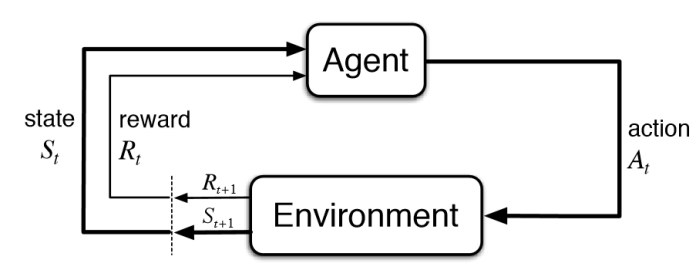
\includegraphics[width=.7\textwidth]{figures/reinforcement-learning}
\end{center}
\caption{The agent-environment interaction in a Markov decision process.}
\label{fig:mdp}
\end{figure}


\subsection{Markov property}


Suppose that the agent is in state \state{t}\ takes action \action{t}\ at time $t$.
Then the agent receives reward \reward{t+1}\ (from the environment) and the environment transitions to state \state{t+1}.
MDP assumes that all these quantities are random variables.

Let \stateset\ and \actionset\ be the set of all the states and that of all the actions the agent can take respectively.

Now suppose that the environment is in state $\state{0}\in\stateset$ the agent takes action $\action{0}\in\actionset$ at $t=0$.
Then the state of the environment becomes $\state{1}\in\stateset$ giving the agent $\reward{1}\in\reals$ as reward.
Suppose that the agent repeat taking actions.

Then we have a sequence of random variables
\begin{equation}
\state{0}, \action{0},
\reward{1}, \state{1}, \action{1},
\reward{2}, \state{2}, \action{2},
\reward{3}, \state{3}, \action{3},
\ldots
\end{equation}

We assume that these random variables satisfy the Markov Property (as assumed by the name) in the following sense.

\begin{equation}
\state{t+1}, \reward{t+1} | \state{t}, \action{t}, \reward{t}, \state{t-1}, \action{t-1}, \reward{t-1}, \ldots
= \state{t+1}, \reward{t+1} | \state{t}, \action{t}
\end{equation}
\ie, two random variables, \state{t+1}\ and \reward{t+1}, conditioned on every state, action, and reward before $t+1$
are the same as those conditioned on \state{t}\ and \reward{t}\ only.

This can be formally expressed using the probability density function (PDF)
as follows.
\begin{equation}
\condprobbig{\state{t+1}, \reward{t+1} }{ \state{t}, \action{t}, \reward{t}, \state{t-1}, \action{t-1}, \reward{t-1}, \ldots}
= \condprobbig{\state{t+1}, \reward{t+1} }{ \state{t}, \action{t} }.
\end{equation}

This is the reason that the process is called \emph{Markov} decision process.

\subsection{Policy}

The \emph{policy} is defined by the conditional probability of \action{t}\ given \state{t},
\ie,
\begin{equation}
\pol(A|S) = \condprobb{A_t}{\state{t}},
\end{equation}
which implies the probability of taking certain action depends only on the current state, not the time.
The policy decides which actions the agent takes in each state.

Let \polset\ be the set of all the policies.

\subsection{Return}

The \emph{return} at $t$ is defined by
\begin{equation}
        G_t
        = \sum_{k=0}^\infty \gamma^k \reward{t+k}
        = \reward{t+1} + \gamma \reward{t+2} + \gamma^2 \reward{t+3} + \cdots
\end{equation}
where $\gamma \in [0,1]$ is called the \emph{discount factor}.
If $\gamma=0$, the agent is myopic, \ie, it only cares the immediate reward.
If $\gamma=1$, the agent is truly far-sighted, \ie, it cares all the future rewards without discounting.
If $\gamma$ is somewhere between $0$ and $1$, it considers near-future rewards more importantly than those in far future.


\subsection{State value function and action value function}

The state value function (which is sometimes referred to as just value function) is defined by
\begin{equation}
v_\pol(\curs)
= \Expect_{\pol,p} \condsetbig{G_{t}}{\state{t} = \curs}
= \Expect_{\pol,p} \condsetbig{
    \sum_{k=0}^\infty \gamma^k \reward{t+k}
    }{\state{t} = \curs}.
\end{equation}
In other words, the state value function is a function of a state
representing the expected return the agent will get from the state
when following the policy $\pol$.

The action value function (which is sometimes referred to as just action function) is defined by
\begin{equation}
q_\pol(\curs, \cura)
= \Expect_{\pol,p} \condsetbig{G_{t}}{\state{t} = \curs, A_t = \cura}
= \Expect_{\pol,p} \condsetbig{
    \sum_{k=0}^\infty \gamma^k \reward{t+k}
    }{\state{t} = \curs, A_t = \cura}.
\end{equation}
In other words, the action value function is a function of a state and an action
representing the expected return the agent will get from the state when the agent takes a certain action
and follows the policy $\pol$.

As mentioned above, most reinforcement learning algorithms try to maximize either one of these functions,
\ie,
not maximizing the immediate reward, but the long-term return.

%\newpage
\section{Bellman equation}

\href{https://en.wikipedia.org/wiki/Richard_E._Bellman}{Richard E. Bellman}, who introduced dynamic programming in $1953$,
proposed an equation as a necessary condition for optimality associated with dynamic programming,
which is called Bellman equation.
One of the properties that Markov property implies is that the value functions only depend on the current state (and the action taken)
and that the function value is closely related to the function values of the next states.
These facts are cleverly used to derive the Bellman equation.
Here we introduce two Bellman equations; one for the state value function and the other for action value function.


\subsection{Bellman equations}

To derive Bellman equations, we use some basic statistics facts regarding conditional expectations.
(Refer to \S\ref{sec:rl-app}.)

Since the definitions of state value function and action value function together with (\ref{eq:dkci}) imply
\begin{eqnarray*}
v_\pol(\curs)
&=& \Expect_{\pol,p} \condsetbig{G_{t}}{\state{t} = \curs}
\\
&=& \Expect_{A_t|\state{t} =\curs} \Expect_{\pol,p} \condsetbig{G_{t}}{\state{t} = \curs, A_t}
\\
&=& \sum_\cura p(A_t=\cura|\state{t} =\curs) \Expect_{\pol,p} \condsetbig{G_{t}}{\state{t} = \curs, A_t=\cura}
\\
&=& \sum_\cura \pol(\cura|\curs) \Expect_{\pol,p} \condsetbig{G_{t}}{\state{t} = \curs, A_t=\cura}
\\
&=& \sum_\cura \pol(\cura|\curs) q_\pol(\curs,\cura)
\end{eqnarray*}
and
\begin{eqnarray*}
q_\pol(\curs, \cura)
&=& \Expect_{\pol,p} \condsetbig{G_{t}}{\state{t} = \curs, A_t = \cura}
\\
&=& \Expect_{\state{t+1}, \reward{t+1}|\state{t}=\curs,A_t=\cura} \Expect_{\pol,p} \condsetbig{G_{t}}{\state{t} = \curs, A_t = \cura, \state{t+1}, \reward{t+1} }
\\
&=& \Expect_{\state{t+1}, \reward{t+1}|\state{t}=\curs,A_t=\cura} \Expect_{\pol,p} \condsetbig{\sum_{k=0}^\infty \df^k \reward{t+k+1}}{\state{t} = \curs, A_t = \cura, \state{t+1}, \reward{t+1} }
\\
&=& \Expect_{\state{t+1}, \reward{t+1}|\state{t}=\curs,A_t=\cura} \Expect_{\pol,p} \condsetbig{\reward{t+1} + \df \sum_{k=0}^\infty \df^k \reward{t+k+2}}{\state{t} = \curs, A_t = \cura, \state{t+1}, \reward{t+1} }
\\
&=& \sum_{\nexts, r} p_{\state{t+1}, \reward{t+1}|\state{t},A_t}(\nexts, r|\curs,\cura) \Expect_{\pol,p} \condsetbig{\reward{t+1} + \df G_{t+1} }{\state{t} = \curs, A_t = \cura, \state{t+1} = \nexts, \reward{t+1} =r}
\\
&=& \sum_{\nexts, r} p_{\state{t+1}, \reward{t+1}|\state{t},A_t}(\nexts, r|\curs,\cura) \left( r + \df \Expect_{\pol,p} \condsetbig{G_{t+1}}{\state{t} = \curs, A_t = \cura, \state{t+1} = \nexts, \reward{t+1} =r} \right)
\\
&=& \sum_{\nexts, r} p_{\state{t+1}, \reward{t+1}|\state{t},A_t}(\nexts, r|\curs,\cura) \left( r + \df \Expect_{\pol,p} \condsetbig{G_{t+1}}{\state{t+1} = \nexts} \right)
\\
&=& \sum_{\nexts, r} p_{\state{t+1}, \reward{t+1}|\state{t},A_t}(\nexts, r|\curs,\cura) \left( r + \df v_\pol(\nexts) \right),
\end{eqnarray*}
we have the following two equations relating state value function to action value function and vise versa.
\begin{equation}
\label{eq:rel:v-a}
v_\pol(\curs) = \sum_\cura \pol(\cura|\curs) q_\pol(\curs,\cura).
\end{equation}
\begin{equation}
\label{eq:rel:a-v}
q_\pol(\curs, \cura)
= \sum_{\nexts, r} p_{\state{t+1}, \reward{t+1}|\state{t},A_t}(\nexts, r|\curs,\cura) \left( r + \df v_\pol(\nexts) \right).
\end{equation}

Now (\ref{eq:rel:v-a}) and (\ref{eq:rel:a-v}) imply that
\begin{equation}
\label{eq:bellman:state}
v_\pol(\curs)
= \sum_\cura \pol(\cura|\curs) q_\pol(\curs,\cura)
= \sum_\cura \pol(\cura|\curs) \sum_{\nexts, r} p(\nexts, r|\curs,\cura) \left( r + \df v_\pol(\nexts) \right)
\end{equation}
and
\begin{equation}
\label{eq:bellman:action}
q_\pol(\curs,\cura)
= \sum_{\nexts, r} p(\nexts, r|\curs,\cura) \left( r + \df v_\pol(\nexts) \right)
= \sum_{\nexts, r} p(\nexts, r|\curs,\cura) \left( r + \df \sum_\nexta \pol(\nexta|\nexts) q_\pol(\nexts,\nexta) \right).
\end{equation}

The equation (\ref{eq:bellman:state}) is called \emph{Bellman equation for state value function}
and the equation (\ref{eq:bellman:action}) is called \emph{Bellman equation for action value function}.

\subsection{Bellman optimality equations}

Now suppose that the policy \optpol\ is the optimal policy.
Then we define the \emph{optimal state-value function}
as that of \optpol, \ie,
\begin{equation}
v_\ast(\curs) = v_{\optpol}(\curs) = \max_{\pol\in\polset} v_\pol(\curs).
\end{equation}
Likewise,
we define the \emph{optimal action-value function}
as that of \optpol, \ie,
\begin{equation}
q_\ast(\curs,\cura) = q_{\optpol}(\curs,\cura) = \max_{\pol\in\polset} q_\pol(\curs,\cura).
\end{equation}

Then (\ref{eq:rel:v-a}) and (\ref{eq:rel:a-v}) imply that
\begin{equation}
\label{eq:bellman:opt:state}
v_\ast(\curs) = v_{\optpol}(\cura) = \max_{\cura\in\actionset} q_{\optpol}(\curs,\cura)
= \max_{\cura\in\actionset} \sum_{\nexts, r} p(\nexts, r|\curs,\cura) \left( r + \df v_\pol(\nexts) \right).
\end{equation}
and
\begin{equation}
\label{eq:bellman:opt:action}
q_\ast(\curs,\cura)
= q_{\optpol}(\curs,\cura)
= \sum_{\nexts, r} p(\nexts, r|\curs,\cura) \left( r + \df v_{\optpol}(\nexts) \right).
= \sum_{\nexts, r} p(\nexts, r|\curs,\cura) \left( r + \df \max_{\nexta\in\actionset}q_{\optpol}(\nexts, \nexta) \right).
\end{equation}

The equation (\ref{eq:bellman:opt:state}) is called \emph{Bellman optimality equation for state value function}
and the equation (\ref{eq:bellman:opt:action}) is called \emph{Bellman optimality equation for action value function}.


%\newpage
\section{Dynamic programming}

The term dynamic programming (DP)
refers to a collection of algorithms that
can be used to compute optimal policies given a perfect model of the environment as a Markov decision process (MDP).
DP provides an essential foundation for the understanding of the methods presented in the rest of this chapter.
All of these methods can be viewed as attempts to achieve much the same effect as DP,
only with less computation and without assuming a perfect model of the environment.

The key idea of DP, and of reinforcement learning generally, is the use of value functions to organize and structure the search for good policies.


\subsection{Policy evaluation (prediction)}

We consider how to compute the state-value function $v_\pol$ for an arbitrary policy \pol.
This is called \emph{policy evaluation} in the DP literature. We also refer to it as the \emph{prediction problem}.
The existence and uniqueness of $v_\pol$ are guaranteed as long as either $\df < 1$
or eventual termination is guaranteed from all states under the policy $\pol$.

The policy evaluation algorithm uses the fact that all the state value functions satisfy the Bellman equation for state value function.
We use this equation, but in an iterative manner.
\begin{equation}
v_{k+1}(\curs)
\assign \sum_\cura \pol(\cura|\curs) \sum_{\nexts, r} p(\nexts, r|\curs,\cura) \left( r + \df v_{k}(\nexts) \right).
\end{equation}
This equation resembles (\ref{eq:bellman:state}), but different because now we put subscript $k$ in place of the policy \pol.
Indeed, the sequence $v_k$
can be shown in general to converge to $v_\pol$ as $k$ goes to $\infty$
the same conditions that guarantee the existence of $v_\pol$.
This algorithm is called \emph{iterative policy evaluation}.

We can consider \emph{in-place} version of this algorithm,
\ie, we replace the values for $v_k$ for each state without waiting until we sweep all the states for one iteration.
This in-place algorithm also converges to $v_\pol$.
In fact, it usually converges faster.
This in-place algorithm is described in \tablename~\ref{tab:alg:policy-evaluation}.


\begin{table}
\beginalg
Inputs: \pol, MDP \\
Algorithm parameters: $\theta > 0$ (small threshold determining accuracy of estimation)\\
\\
Initialize $V(\curs) \in \reals$ for all $\curs \in \stateset$ except that $V(\mathrm{terminal}) = 0$ \\
\\
 Loop: \\
 \> $\Delta \assign 0$ \\
 \> For each $s\in\stateset$: \\
 \> \> $v\assign V(\curs)$ \\
 \> \> $V(s) \assign \sum_\cura \pol(\cura|\curs) \sum_{\nexts, r} p(\nexts, r|\curs,\cura) \left( r + \df V(\nexts) \right)$ \\
 \> \> $\Delta \assign \max\{\Delta, |v-V(s)|\}$ \\
 until $\Delta < \theta$
\endalg
\caption{Iterative Policy Evaluation for estimating $V \sim v_\pol$}
\label{tab:alg:policy-evaluation}
\end{table}


\subsection{Policy iteration}

The policy iteration is the iterative process of improving policy as to maximize the value functions.
The algorithm is described in \tablename~\ref{tab:eq:policy-iteration}.

\begin{table}
\beginalg
Inputs: MDP \\
Algorithm parameters: $\theta > 0$ (small threshold determining accuracy of estimation)\\
\\
1. Initialization \\
\> $V(\curs) \in \reals$ and $\pol(s) \in \actionset(s)$ for all $s\in\stateset$\\
\\
2. Policy Evaluation\\
\> Loop: \\
\> \> $\Delta \assign 0$ \\
\> \> For each $s\in\stateset$: \\
\> \> \> $v\assign V(\curs)$ \\
\> \> \> $V(s) \assign \sum_\cura \pol(\cura|\curs) \sum_{\nexts, r} p(\nexts, r|\curs,\cura) \left( r + \df V(\nexts) \right)$ \\
\> \> \> $\Delta \assign \max\{\Delta, |v-V(s)|\}$ \\
\> until $\Delta < \theta$\\
\\
3. Policy Improvement\\
$u \assign {\tt true}$\\
\> For each $\curs \in \stateset$\\
\> \> $b \assign \pol(\curs)$\\
\> \> $\pol(\curs) \assign \sum_\cura \pol(\cura|\curs) \sum_{\nexts, r} p(\nexts, r|\curs,\cura) \left( r + \df v_\pol(\nexts) \right)$\\
\> \> If $b \neq \pol(\curs)$, then $t \assign {\tt false}$\\
\> If $u$, then stop and return $V \sim v_\ast$ and $\pol \sim \optpol$; else go to 2
\endalg
\caption{Policy Iteration (using iterative policy evaluation) for estimating $\pol \sim \optpol$.}
\label{tab:eq:policy-iteration}
\end{table}


\subsection{Value iteration}

One drawback to policy iteration is that each of its iterations involves policy evaluation.
In fact, the policy evaluation step of policy iteration can be truncated in several ways
without losing the convergence guarantees of policy iteration.
One important special case is when policy evaluation is stopped after just one sweep (one update of each state).
This algorithm is called \emph{value iteration}.
It can be written as a particularly simple update operation that combines the policy improvement and truncated policy evaluation steps.
\begin{equation}
v_{k+1}(\curs) \assign \max_{\cura\in\actionset} \sum_{\nexts, r} p(\nexts, r|\curs,\cura) \left( r + \df v_k(\nexts) \right).
\end{equation}
Note that value iteration is obtained simply by turning the Bellman optimality equation for state value function
(\ref{eq:bellman:opt:state})
into an update rule.

The in-place version of value iteration algorithm is described in \tablename~\ref{tab:alg:value-iteration}.

\begin{table}
\beginalg
Inputs: MDP \\
Algorithm parameters: $\theta > 0$ (small threshold determining accuracy of estimation)\\
\\
Initialize $V(\curs) \in \reals$ for all $\curs \in \stateset$ except that $V(\mathrm{terminal}) = 0$ \\
\\
Loop: \\
\> $\Delta \assign 0$ \\
\> For each $s\in\stateset$: \\
\> \> $v\assign V(\curs)$ \\
\> \> $V(s) \assign \max_{\cura\in\actionset(\curs)} \sum_{\nexts, r} p(\nexts, r|\curs,\cura) \left( r + \df V(\nexts) \right)$ \\
\> \> $\Delta \assign \max\{\Delta, |v-V(s)|\}$ \\
until $\Delta < \theta$\\
\\
Output: deterministic policy $\pol$ such that\\
\> $\pol(\curs) = \argmax_{\cura\in\actionset(\curs)} \sum_{\nexts, r} p(\nexts, r|\curs,\cura) \left( r + \df V(\nexts) \right)$
\endalg
\caption{Value Iteration for estimating $\pol \sim \optpol$}
\label{tab:alg:value-iteration}
\end{table}



%\newpage
\section{Monte Carlo methods}

Here we consider learning methods for estimating value functions and discovering optimal policies.
Unlike the previous methods,
we do not assume complete knowledge of the environment.
Monte Carlo (MC) methods require only experience sample sequences of states, actions, and rewards
from \emph{actual or simulated interaction with an environment}.
Learning from actual experience is striking because it requires no prior knowledge of the environment’s dynamics,
yet can still attain optimal behavior.
\emph{Learning from simulated experience is also powerful.}
Although a model is required,
the model need only generate sample transitions,
\emph{not the complete probability distributions of all possible transitions} that is required for dynamic programming (DP).

MC methods are ways of solving the reinforcement learning problem based on averaging sample returns.
To ensure that well-defined returns are available, here we define Monte Carlo methods only for episodic tasks.

Monte Carlo methods sample and average returns for each state–action pair much like the bandit methods
where we sample and average rewards for each action.
The main difference is that now there are multiple states,
each acting like a different bandit problem (like an associative-search or contextual bandit)
and the different bandit problems are interrelated.
That is, the return after taking an action in one state depends on the actions taken in later states in the same episode.
Because all the action selections are undergoing learning, the problem becomes nonstationary from the point of view of the earlier state.


To handle the nonstationarity,
we adapt the idea of general policy iteration (GPI) developed for DP.
Whereas there we computed value functions from knowledge of the MDP,
here we learn value functions from sample returns with the MDP.
The value functions and corresponding policies still interact to attain optimality
in essentially the same way (GPI).
As in DP,
first we consider the prediction problem, then policy improvement, and, finally,
the control problem and its solution by GPI.
Each of these ideas taken from DP is extended to the Monte Carlo case in which only sample experience is available.


\subsection{Monte Carlo prediction}

An obvious way to estimate it from experience, then, is simply to average the returns observed after visits to that state.
There are two Monte Carlo (MC) prediction methods; \emph{first-visit MC method} and \emph{every-visit MC method}.
These two MC methods are very similar but have slightly different theoretical properties.
First-visit MC has been most widely studied, dating back to the 1940s.
Every-visit MC extends more naturally to function approximation and eligibility traces.

\tablename~\ref{tab:alg:first-visti-mc-prediction} describes the first-visit MC prediction algorithm.


\begin{table}
\beginalg
Inputs: \pol\\
\\
Initialize:\\
\> $V(\curs) \in \reals$ for all $\curs\in\stateset$\\
\> $R(\curs) \assign {\tt list()}$ for all $\curs\in\stateset$\\
\\
Loop: \\
\> Generate an episode following \pol: $\state{0}, \action{0}, \reward{1}, \state{1}, \action{1}, \reward{2}, \ldots, \state{T-1}, \action{T-1}, \reward{T}$\\
\> $G \assign 0$\\
\> Loop for each step of episode, $t+T-1, T-2, \ldots, 0$:\\
\> \> $G \assign \df G + \reward{t+1}$\\
\> \> If $\state{t} \not\in \{\state{0}, \state{1}, \ldots, \state{t-1}\}$:\\
\> \> \> $R(\state{t}){\tt.append}(G)$\\
\> \> \> $V(\state{t}) \assign R(\state{t}){\tt .average()}$\\
Until a certain criterion is satisfied
\endalg
\caption{First-visit MC prediction for estimating $V \sim v_\pol$}
\label{tab:alg:first-visti-mc-prediction}
\end{table}


\subsection{Monte Carlo control}

The overall idea is to proceed according to the same pattern as in the dynamic programming, \ie,
according to the idea of generalized policy iteration (GPI).
In GPI one maintains both an approximate policy and an approximate value function.
The value function is repeatedly altered to more closely approximate
the value function for the current policy,
and the policy is repeatedly improved with respect to the current value function.
These two kinds of changes work against each other to some extent,
as each creates a moving target for the other,
but together they cause both policy and value function to approach optimality.

For Monte Carlo policy evaluation
it is natural to alternate between evaluation and improvement on an episode-by-episode basis.
After each episode,
the observed returns are used for policy evaluation,
and then the policy is improved at all the states visited in the episode.
A complete simple algorithm along these lines, which is called Monte Carlo ES for Monte Carlo with Exploring Starts,
is described in \tablename~\ref{tab:alg:mc-es-control}.


\begin{table}
\beginalg
Initialize:\\
\> $\pol(\curs) \in \actionset(\curs)$ for all $\curs\in\stateset$\\
\> $Q(\curs,\cura) \in \reals$ for all $\curs\in\stateset$ and $\cura\in\actionset(\curs)$\\
\> $R(\curs, \cura) \assign {\tt list()}$ for all $\curs\in\stateset$ and $\cura\in\actionset(\curs)$\\
\\
Loop: \\
\> Choose $\state{0} \in \stateset$, $\action{0} \in \actionset(\state{0})$ randomly such that all pairs have probability $> 0$\\
\> Generate an episode from \state{0}, \action{0}\ following \pol: $\state{0}, \action{0}, \reward{1}, \state{1}, \action{1}, \reward{2}, \ldots, \state{T-1}, \action{T-1}, \reward{T}$\\
\> $G \assign 0$\\
\> Loop for each step of episode, $t+T-1, T-2, \ldots, 0$:\\
\> \> $G \assign \df G + \reward{t+1}$\\
\> \> If $\state{t} \not\in \{\state{0}, \state{1}, \ldots, \state{t-1}\}$:\\
\> \> \> $R(\state{t}, A_t){\tt.append}(G)$\\
\> \> \> $Q(\state{t}, A_t) \assign R(\state{t}, A_t){\tt .average()}$\\
\> \> \> $\pol(\state{t}) \assign \argmax_{\cura\in\actionset(\state{t})} Q(\state{t}, \cura)$\\
Until a certain criterion is satisfied
\endalg
\caption{MC ES (exploring starts) for estimating $\pol \sim \optpol$}
\label{tab:alg:mc-es-control}
\end{table}



\subsection{Monte Carlo control without exploring starts}


How can we avoid the unlikely assumption of exploring starts?
The only general way to ensure that all actions are selected infinitely often
is for the agent to continue to select them.
There are two approaches to ensuring this,
resulting in what we call on-policy methods and off-policy methods.
On-policy methods attempt to evaluate or improve the policy
that is used to make decisions,
whereas off-policy methods evaluate or improve a policy different from
that used to generate the data.
The Monte Carlo ES method developed above is
an example of an on-policy method.
In this section we show how an on-policy Monte Carlo control method
can be designed that does not use the unrealistic assumption of exploring starts.

The on-policy first-visit MC control using \epsgreedy\
is described in \tablename~\ref{tab:alg:on-pol-ms-control}.


\begin{table}
\beginalg
Algorithm parameters: small $\epsilon>0$\\
\\
Initialize:\\
\> $\pol(\curs) \in \actionset(\curs)$ for all $\curs\in\stateset$\\
\> $Q(\curs,\cura) \in \reals$ for all $\curs\in\stateset$ and $\cura\in\actionset(\curs)$\\
\> $R(\curs, \cura) \assign {\tt list()}$ for all $\curs\in\stateset$ and $\cura\in\actionset(\curs)$\\
\\
Loop: \\
\> Choose $\state{0} \in \stateset$, $\action{0} \in \actionset(\state{0})$ randomly such that all pairs have probability $> 0$\\
\> Generate an episode from \state{0}, \action{0}\ following \pol: $\state{0}, \action{0}, \reward{1}, \state{1}, \action{1}, \reward{2}, \ldots, \state{T-1}, \action{T-1}, \reward{T}$\\
\> $G \assign 0$\\
\> Loop for each step of episode, $t+T-1, T-2, \ldots, 0$:\\
\> \> $G \assign \df G + \reward{t+1}$\\
\> \> If $\state{t} \not\in \{\state{0}, \state{1}, \ldots, \state{t-1}\}$:\\
\> \> \> $R(\state{t}, A_t){\tt.append}(G)$\\
\> \> \> $Q(\state{t}, A_t) \assign R(\state{t}, A_t){\tt .average()}$\\
\> \> \> $A^\ast \assign \argmax_{\cura\in\actionset(\state{t})}$\\
\> \> \> For all $\cura \in \actionset(\state{t})$\\
\> \> \> \> $\pol(\cura|\state{t}) \assign \left\{\begin{array}{ll}
1-\epsilon + \epsilon / |\actionset(\state{t})| & \mbox{if } \cura = A^\ast\\
\epsilon / |\actionset(\state{t})| & \mbox{if } \cura \neq A^\ast
\end{array}\right.$\\
Until a certain criterion is satisfied
\endalg
\caption{On-policy first-visit MC control (for \epssoft\ policies) for estimating $\pol \sim \optpol$}
\label{tab:alg:on-pol-ms-control}
\end{table}



\subsection{Off-policy prediction via important sampling}

XXX

\subsection{Off-policy Monte Carlo control}

XXX


%\newpage
\section{Temporal-difference learning}

Temporal-difference (TD) learning is a combination of Monte Carlo ideas and dynamic programming (DP) ideas.
Like Monte Carlo methods,
TD methods can learn directly from raw experience without a model of the environment’s dynamics.
Like DP, TD methods update estimates based in part on other learned estimates,
without waiting for a final outcome (they bootstrap).
The relationship between TD, DP, and Monte Carlo methods
is a recurring theme in the theory of reinforcement learning.

We start by focusing on the policy evaluation or prediction problem,
the problem of estimating the value function $v_\pol$ for a given policy \pol.
For the control problem (finding an optimal policy),
DP, TD, and Monte Carlo methods all use some variation of generalized policy iteration (GPI).


\subsection{TD prediction}

Both TD and Monte Carlo methods use experience to solve the prediction problem.
A simple every-visit MC method suitable for nonstationary environments is
\begin{equation}
V(\state{t}) \assign
V(\state{t}) + \alpha(G_t - V(\state{t}))
= (1-\alpha) V(\state{t}) + \alpha G_t.
\end{equation}


TD methods need to wait only until the next time step.
At time $t + 1$,
they immediately form a target and make a useful update using the observed reward \reward{t +1}\
and the estimate $V( \state{t +1})$. The simplest TD method makes the update
\begin{equation}
\label{eq:one-step-update}
V(\state{t}) \assign
V(\state{t}) + \alpha ( \reward{t+1} + \df V(\state{t+1}) - V(\state{t}))
= (1-\alpha) V(\state{t}) + \alpha ( \reward{t+1} + \df V(\state{t+1})).
\end{equation}

This TD method is called TD(0),
or one-step TD,
because it is a special case of the TD(\tdparam)
and $n$-step TD methods.
\tablename~\ref{tab:alg:td-0} specifies TD(0) completely in procedural form.


\begin{table}
\beginalg
Inputs: the policy \pol\ to be evaluated\\
Algorithm parameters: step size $\alpha\in(0,1]$\\
\\
Initialize:\\
\>$V(\curs) \in \reals$ for all $\curs \in \stateset$ except that $V(\mathrm{terminal}) = 0$ \\
\\
Loop for each episode:\\
\> Initialize $S$\\
\> Loop for each step of episode:\\
\> \> $A \assign \mbox{ action given by } \pol \mbox{ for } S$\\
\> \> Take action $A$, observe $R$, $S'$\\
\> \> $V(S) \assign (1-\alpha) V(S) + \alpha(R + \df V(S'))$\\
\> \> $S \assign S'$\\
\> until $S$ is terminal\\
Until a certain criterion is satisfied
\endalg
\caption{TD(0) for estimating $v_\pol$}
\label{tab:alg:td-0}
\end{table}


The quantity in brackets in the TD(0) update is a sort of error,
measuring the difference between the estimated value of \state{t}\
and the better estimate $\reward{t+1} + \df V(\state{t+1})$.
This quantity, called the TD error, arises in various forms throughout reinforcement learning.
It can be formally defined as follows.
\begin{equation}
\label{eq:one-step-error}
\tderror{t} \defeq \reward{t+1} + \df V_t(\state{t+1}) - V_t(\state{t})
\end{equation}

It is interesting to observe that we can express Monte Carlo error in terms of modified TD errors
if we defined the modified TD error as follows.
\begin{equation}
\label{eq:one-step-error-var}
\tderrorvar{t} \defeq \reward{t+1} + \df V_{t+1}(\state{t+1}) - V_t(\state{t})
\end{equation}

Then the Monte Carlo error is defined by $\return{t} - V_t(\state{t})$ is
\begin{eqnarray}
\return{t} - V_t(\state{t})
&=& \reward{t+1} + \df \return{t+1} - V_t(\state{t})
\nonumber
\\
&=& \reward{t+1} + \df \left( \return{t+1} - V_{t+1}(\state{t+1}) + V_{t+1}(\state{t+1}) \right) - V_t(\state{t})
\nonumber
\\
&=& \reward{t+1} + \df V_{t+1}(\state{t+1}) - V_t(\state{t}) + \df \left( \return{t+1} - V_{t+1}(\state{t+1})\right)
\nonumber
\\
&=& \tderrorvar{t} + \df \left( \return{t+1} - V_{t+1}(\state{t+1})\right)
\nonumber
\\
&=& \tderrorvar{t} + \df \tderrorvar{t+1} + \df^2 \left( \return{t+2} - V_{t+2}(\state{t+2})\right)
\nonumber
\\
&=& \tderrorvar{t} + \df \tderrorvar{t+1} + \df^2 \tderrorvar{t+2} + \cdots
+ \df^{T-t-2} \tderrorvar{T-2} + \df^{T-t-1} \left( \return{T-1} - V_{T-1}(\state{T-1})\right)
\nonumber
\\
&=& \tderrorvar{t} + \df \tderrorvar{t+1} + \df^2 \tderrorvar{t+2} + \cdots
+ \df^{T-t-2} \tderrorvar{T-2} + \df^{T-t-1} \left( \reward{T} + \df V_{T}(\state{T}) - V_{T-1}(\state{T-1})\right)
\nonumber
\\
&=& \tderrorvar{t} + \df \tderrorvar{t+1} + \df^2 \tderrorvar{t+2} + \cdots
+ \df^{T-t-2} \tderrorvar{T-2} + \df^{T-t-1} \tderrorvar{T-1}
\nonumber
\\
&=& \sum_{k=t}^{T-1} \df^{k-t} \tderrorvar{k}
= \sum_{k=0}^{T-t-1} \df^{k} \tderrorvar{k+t}
\label{eq:monte-error-sum-of-tderrorvar}
\end{eqnarray}
where the fact that the state-value function for a terminal state, $V_{T-1}(\state{T})$, is $0$ is used.

This means the Monte Carlo error, \ie, the difference between the return along the path from $t$ to a terminal state of the episode
and the state-value function of \state{t}\ can be expressed as sum of discounted (modified) one-step TD errors.
If we assume that every $V_t$ does not change during the episode, \tderror{t}\ coincides with \tderrorvar{t}.
Hence (\ref{eq:monte-error-sum-of-tderrorvar}) becomes
\begin{equation}
\label{eq:monte-error-sum-of-tderror}
\return{t} - V(\state{t})
= \sum_{k=t}^{T-1} \df^{k-t} \tderror{k}
= \sum_{k=0}^{T-t-1} \df^{k} \tderror{k+t}.
\end{equation}



\subsection{Sarsa: on-policy TD Control}

As in all on-policy methods,
we continually estimate $q_\pol$ for the behavior policy \pol,
and at the same time change \pol\ toward greediness with respect to $q_\pol$.

The convergence properties of the Sarsa algorithm depend on the nature of the policy’s dependence on $Q$.
For example, one could use $\epsilon$ greedy or \epssoft\ policies.
Sarsa converges with probability $1$ to an optimal policy and action-value function
as long as all state–action pairs are visited an infinite number of times
and the policy converges in the limit to the greedy policy
(which can be arranged, for example, with \epsgreedy\ policies by setting $\epsilon = 1 /t$).

This algorithm is described in \tablename~\ref{tab:alg:sarsa}.


\begin{table}
\beginalg
Algorithm parameters: step size $\alpha \in (0, 1]$ and small $\epsilon>0$\\
\\
Initialize:\\
\> $Q(\curs,\cura) \in \reals$ for all $\curs\in\stateset$ and $\cura\in\actionset(\curs)$
    except $Q(\mathrm{terminal}, \cdot)=0$\\
\\
Loop for each episode:\\
\> Initialize $S$\\
\> Choose $A$ from $S$ using policy derived from $Q$ (\eg, \epsgreedy)\\
\> Loop for each step of episode:\\
\> \> Take action $A$, observe $R$, $S'$\\
\> \> Choose $A'$ from $S'$ using policy derived from $Q$ (\eg, \epsgreedy)\\
\> \> $Q(S,A) \assign (1-\alpha) Q(S,A) + \alpha (R + \df Q(S',A'))$\\
\> \> $S \assign S'$, $A \assign A'$,\\
\> until $S$ is terminal\\
Until a certain criterion is satisfied
\endalg
\caption{Sarsa (on-policy TD control) for estimating $Q\sim q_\ast$}
\label{tab:alg:sarsa}
\end{table}


\subsection{Q-learning: off-policy TD control}

One of the early breakthroughs in reinforcement learning was
the development of an off-policy TD control algorithm known as Q-learning (Watkins, 1989),
defined by
\begin{eqnarray}
\nonumber
Q(\state{t}, A_t) &\assign&
Q(\state{t}, A_t) + \alpha \left(
\reward{t+1}
+ \df \max_{a} Q(\state{t+1},a) - Q(\state{t},A_t)
\right)
\\&&
=
(1-\alpha) Q(\state{t}, A_t) + \alpha \left(
\reward{t+1}
+ \df \max_{a} Q(\state{t+1},a)
\right).
\end{eqnarray}


The learned action-value function, $Q$, directly approximates $q_\ast$,
the optimal action-value function, independent of the policy being followed
This dramatically simplifies the analysis of the algorithm and enabled early convergence proofs.
The policy still has an effect in that it determines which state–action pairs are visited and updated.
However, all that is required for correct convergence is that all pairs continue to be updated.

Under this assumption and a variant of the usual stochastic approximation conditions
on the sequence of step-size parameters,
$Q$ has been shown to converge with probability $1$ to $q_\ast$.
The Q-learning algorithm is described in \tablename~\ref{tab:alg:q-learning}.



\begin{table}
\beginalg
Algorithm parameters: step size $\alpha \in (0, 1]$ and small $\epsilon>0$\\
\\
Initialize:\\
\> $Q(\curs,\cura) \in \reals$ for all $\curs\in\stateset$ and $\cura\in\actionset(\curs)$
    except $Q(\mathrm{terminal}, \cdot)=0$\\
\\
Loop for each episode:\\
\> Initialize $S$\\
\> Loop for each step of episode:\\
\> \> Choose $A$ from $S$ using policy derived from $Q$ (\eg, \epsgreedy)\\
\> \> Take action $A$, observe $R$, $S'$\\
\> \> $Q(S,A) \assign (1-\alpha) Q(S,A) + \alpha (R + \df \max_{\cura\in\actionset(S')}Q(S',\cura))$\\
\> \> $S \assign S'$\\
\> until $S$ is terminal\\
Until a certain criterion is satisfied
\endalg
\caption{Q-learning (off-policy TD control) for estimating $\pol \sim \optpol$}
\label{tab:alg:q-learning}
\end{table}


\subsection{Maximization bias and double learning}

XXX

%\newpage
\section{$n$-step bootstrapping}
\label{sec:n-step}

There exists another method which unifies
the Monte Carlo (MC) methods and the one-step temporal-difference (TD) methods.
Neither MC methods nor one-step TD methods are always the best.
Here we present $n$-step TD methods that generalize both methods
so that one can shift from one to the other smoothly as needed to meet the demands of a particular task.
$n$-step methods span a spectrum with MC methods at one end and one-step TD methods at the other.
The best methods are often intermediate between the two extremes.

Another way of looking at the benefits of $n$-step methods is
that they free one from the tyranny of the time step.
With one-step TD methods the same time step determines how often the action can be changed
and the time interval over which bootstrapping is done.
In many applications one wants to be able to update the action very fast
to take into account anything that has changed,
but bootstrapping works best if it is over a length of time in which a significant and recognizable state change has occurred.
With one-step TD methods,
these time intervals are the same,
and so a compromise must be made.
$n$-step methods enable bootstrapping to occur over multiple steps,
freeing us from the tyranny of the single time step.

The idea of $n$-step methods is usually used as an introduction to the algorithmic idea of eligibility traces.

\subsection{$n$-step TD prediction}

$n$-step TD prediction is a method lying between Monte Carlo and (one-step) TD method, \ie, TD(0).
Consider estimating $v_\pol$ from sample episodes generated using $\pol$.
Monte Carlo methods perform an update for each state based on the entire sequence of observed rewards
from that state until the end of the episode.
The update of one-step TD methods, on the other hand,
is based on just the one next reward,
bootstrapping from the value of the state one step later as a proxy for the remaining rewards.

One kind of intermediate method, then, would perform an update based on an intermediate number of rewards:
more than one, but less than all of them until termination.

The methods that use $n$-step updates are still TD methods
because they still change an earlier estimate based on how it differs from a later estimate.
Now the later estimate is not one step later,
but $n$ steps later.
Methods in which the temporal difference extends over $n$ steps are called $n$-step TD methods.

Suppose that the process is episodic, \ie, ever episode ends or enters a terminal state within finite number of steps.
Then the \emph{target} of Monte Carlo update
is the return at time step $t$, \ie,
\begin{equation}
\return{t} = \reward{t+1}
+ \df \reward{t+2}
+ \df^2 \reward{t+3}
+ \cdots
+ \df^{T-t-1} \reward{T}
\end{equation}
where $T$ is the last time step of the episode.

The target of the one-step TD method is the first reward plus the discounted estimated value of the next state, \ie,
\begin{equation}
\label{eq:one-step-return}
\nstepreturn{t}{t+1} = \reward{t+1} + \df V_t(\state{t+1})
\end{equation}
where $V_t:\stateset\to\reals$ is the estimate of $v_\pol(\state{t+1})$ at time $t$.
Note that the second term $\df V_t(\state{t+1})$ is the estimate for $\df \reward{t+2} + \df^2 \reward{t+3} + \cdots + \df^{T-t-1} \reward{T}$,
but using the state-value function estimate of the next state, instead of using future discounted returns.
Thus, this is a bootstrapping.
Likewise, we can define two-step return as a target for the two-step update.
\begin{equation}
\label{eq:two-step-return}
\nstepreturn{t}{t+2} = \reward{t+1} + \df \reward{t+2} + \df^2 V_{t+1}(\state{t+2})
\end{equation}
where $V_{t+1}:\stateset\to\reals$ is the estimate of $v_\pol(\state{t+2})$ at time $t+1$.
Again here the third term $\df^2 V_{t+1}(\state{t+2})$ is the estimate for $\df^2 \reward{t+3} + \cdots + \df^{T-t-1} \reward{T}$
using bootstrapping.
In general, we can define the $n$-step return as the target for the $n$-step update.
\begin{equation}
\label{eq:n-step-return}
\nstepreturn{t}{t+n} = \left\{\begin{array}{ll}
\reward{t+1} + \df \reward{t+2} + \df^2 \reward{t+3} + \cdots + \df^{n-1} \reward{t+n} + \df^n V_{t+n-1}(\state{t+n})
&\mbox{if } t+n < T
\\
\return{t} & \mbox{if } t+n \geq T
\end{array}\right.
\end{equation}
for $t\geq0$.
An $n$-step return can be considered as an approximation to the full return $\return{t}$.

We can consider algorithm with the $n$-step update using this $n$-step return, \ie,
\begin{equation}
\label{eq:n-step-update}
V_{t+n}(\state{t}) \assign V_{t+n-1}(\state{t}) + \stepsize{t+n-1} (\nstepreturn{t}{t+n} - V_{t+n-1}(\state{t}))
= (1-\stepsize{t+n-1}) V_{t+n-1}(\state{t}) + \stepsize{t+n-1} \nstepreturn{t}{t+n}
\end{equation}

Note that this update cannot be performed before time step $t+n$ because only by then, all the rewards necessary to evaluate (\ref{eq:n-step-return})
become available. Also note that (\ref{eq:n-step-update}) is reduced to (\ref{eq:one-step-update}) when $n=1$.
Therefore one-step TD method is a special case of $n$-step TD method.
The $n$-step TD prediction is described in \tablename~\ref{tab:alg:n-step-td-prediction},
a Pythonian version of which is described in \tablename~\ref{tab:alg:n-step-td-prediction-python-style}.



\begin{table}
\beginalg
Inputs: policy \pol\ to be evaluated\\
\\
Algorithm parameters: step size $\alpha_t \in (0, 1]$ and $n\in\naturals$\\
\\
Initialize:\\
\> $V(s)\in\reals$ for all $\curs\in\stateset$ except that $V(\mathrm{terminal})=0$\\
\\
Loop for each episode:\\
\> Initialize and store $\state{0}$\\
\> $T \assign \infty$\\
\> Loop for each $t=0,1,2,\ldots$:\\
\> \> If $t<T$:\\
\> \> \> $A_t \assign \mbox{ action given by } \pol(\cdot|\state{t})$\\
\> \> \> Take action $A_t$, observe \reward{t+1}, \state{t+1}\\
\> \> \> If $\state{t+1}$ is terminal:\\
\> \> \> \> $T \assign t+1$\\
\> \> $\tau \assign t-n+1$\\
\> \> If $\tau \geq 0$:\\
\> \> \> $G \assign \sum_{i=\tau+1}^{\min\{\tau+n,T\}} \df^{i-\tau-1} \reward{i}$\\
\> \> \> If $\tau+n < T$:\\
\> \> \> \> $G \assign G + \df^{n} V(\state{\tau+n})$\\
\> \> \> $V(\state{\tau}) \assign (1-\stepsize{t}) V(\state{\tau}) + \stepsize{t} G$\\
\> while $\tau<T-1$\\
Until a certain criterion is satisfied
\endalg
\caption{$n$-step TD for estimating $V\sim v_\pol$}
\label{tab:alg:n-step-td-prediction}
\end{table}



\begin{table}
\beginalg
Inputs: policy \pol\ to be evaluated\\
\\
Algorithm parameters: step size $\alpha_t \in (0, 1]$ and $n\in\naturals$\\
\\
Initialize:\\
\> $V(s)\in\reals$ for all $\curs\in\stateset$ except that $V(\mathrm{terminal})=0$\\
\> ${\tt w\_list} = [1, \df, \ldots, \df^{n}]$\\
\\
Loop for each episode:\\
\> ${\tt S\_list} \assign {\tt list()}$, ${\tt R\_list} \assign {\tt list()}$\\
\> Initialize $S$\\
\> ${\tt S\_list.append}(S)$, ${\tt not\_terminated} \assign True$\\
\> Loop for each $t=0,1,2,\ldots$:\\
\> \> If {\tt not\_terminated}:\\
\> \> \> $A \assign \mbox{ action given by } \pol(\cdot|S)$\\
\> \> \> Take action $A$, observe $R$, $S'$\\
\> \> \> ${\tt R\_list.append}(R)$\\
\> \> \> If $S$ is terminal:\\
\> \> \> \> ${\tt not\_terminated} \assign False$\\
\> \> \> else:\\
\> \> \> \> ${\tt S\_list.append}(S')$\\
\> \> \> \> $S \assign S'$\\
\> \> If $t \geq n-1$:\\
\> \> \> ${\tt n\_R\_list} \assign {\tt R\_list}[t-n+1:t+1]$\\
\> \> \> $G \assign {\tt (n\_R\_list * w\_list[:len(n\_R\_list)]).sum()}$\\
\> \> \> If $t+1 < {\tt len(S\_list)}$:\\
\> \> \> \> $G \assign G + {\tt w\_list[-1]} \times V({\tt S\_list}[t+1])$\\
\> \> \> $V({\tt S\_list}[t-n+1]) \assign (1-\stepsize{t}) V({\tt S\_list}[t-n+1]) + \stepsize{t} G$\\
\> while $t-n+1 < {\tt len(R\_list)-1}$\\
Until a certain criterion is satisfied
\endalg
\caption{$n$-step TD for estimating $V\sim v_\pol$ (Pythonic style)}
\label{tab:alg:n-step-td-prediction-python-style}
\end{table}


As the Monte Carlo error can be express as the sum of discounted TD errors,
the $n$-step TD error can be expressed as the sum of the discounted one-step TD errors.
Note that $\nstepreturn{t}{t+n} = \reward{t+1} + \df \nstepreturn{t+1}{t+n}$. Thus,
\begin{eqnarray*}
\nstepreturn{t}{t+n} - V_t(\state{t})
&=& \reward{t+1} + \df \nstepreturn{t+1}{t+n} - V_t(\state{t})
\\
&=& \reward{t+1} + \df \left( \nstepreturn{t+1}{t+n} + V_{t+1}(\state{t+1}) - V_{t+1}(\state{t+1}) \right)- V_t(\state{t})
\\
&=& \reward{t+1} + \df V_{t+1}(\state{t+1}) - V_t(\state{t})
+ \df \left( \nstepreturn{t+1}{t+n} - V_{t+1}(\state{t+1}) \right)
\\
&=& \tderrorvar{t} + \df \left( \nstepreturn{t+1}{t+n} - V_{t+1}(\state{t+1}) \right)
\\
&=& \tderrorvar{t} + \df \tderrorvar{t+1} + \df^2 \left( \nstepreturn{t+2}{t+n} - V_{t+2}(\state{t+2}) \right)
\\
&=& \tderrorvar{t} + \df \tderrorvar{t+1} + \df^2 \tderrorvar{t+2} + \cdots
+ \df^{n-1} \left( \nstepreturn{t+n-1}{t+n} - V_{t+n-1}(\state{t+n-1}) \right)
\\
&=& \tderrorvar{t} + \df \tderrorvar{t+1} + \df^2 \tderrorvar{t+2} + \cdots
+ \df^{n-1} \left( \reward{t+n} + \df V_{t+n-1}(\state{t+n}) - V_{t+n-1}(\state{t+n-1}) \right)
\\
&=& \tderrorvar{t} + \df \tderrorvar{t+1} + \df^2 \tderrorvar{t+2} + \cdots
+ \df^{n-1} \left( \reward{t+n} + \df V_{t+n}(\state{t+n}) - V_{t+n-1}(\state{t+n-1}) \right)
\\
&& + \df^{n} \left( V_{t+n-1}(\state{t+n}) - V_{t+n}(\state{t+n}) \right)
\\
&=& \tderrorvar{t} + \df \tderrorvar{t+1} + \df^2 \tderrorvar{t+2} + \cdots + \df^{n-1} \tderrorvar{t+n-1}
+ \df^{n} \left( V_{t+n-1}(\state{t+n}) - V_{t+n}(\state{t+n}) \right)
\\
&=& \sum_{k=t}^{t+n-1} \df^{k-t}\tderrorvar{k} + \df^{n} \left( V_{t+n-1}(\state{t+n}) - V_{t+n}(\state{t+n}) \right)
\\
&=& \sum_{k=0}^{n-1} \df^{k}\tderrorvar{k+t} + \df^{n} \left( V_{t+n-1}(\state{t+n}) - V_{t+n}(\state{t+n}) \right)
\end{eqnarray*}
where $\tderrorvar{t}$ is defined in (\ref{eq:one-step-error-var}).
Thus, the $n$-step TD error is
\begin{equation}
\nstepreturn{t}{t+n} - V_{t+n-1}(\state{t})
= \sum_{k=0}^{n-1} \df^{k}\tderrorvar{k+t}
+ \df^{n} \left( V_{t+n-1}(\state{t+n}) - V_{t+n}(\state{t+n}) \right)
+ \left(V_t(\state{t}) - V_{t+n-1}(\state{t})\right).
\end{equation}

If $V_t$ does not change during the episode, $\tderror{t} = \tderrorvar{t}$ and $V_{t+n-1}(\state{t+n}) = V_{t+n}(\state{t+n})$,
hence
\begin{equation}
\nstepreturn{t}{t+n} - V(\state{t})
= \sum_{k=t}^{t+n-1} \df^{k-t}\tderror{k}
= \sum_{k=0}^{n-1} \df^{k}\tderror{t+k}
\end{equation}
where $\tderror{t}$ is defined in (\ref{eq:one-step-error}).

The $n$-step return uses the value function $V_{t + n-1}$
to correct for the missing rewards beyond \reward{t+n}.
An important property of $n$-step returns is
that their expectation is guaranteed to be a better estimate of $v_\pol$ than $V_{t+n-1}$ is,
in a worst-state sense.
The worst error of the expected $n$-step return
is guaranteed to be less than or equal to $\df^n$ times the worst error under $V_{t + n - 1}$.

\begin{equation}
\max_{\curs \in \stateset} \left| \Expect_\pol \condsetbig{\nstepreturn{t}{t+n}}{\state{t}=\curs} - v_\pol(\curs) \right|
\leq
\df^n
\max_\curs \left| V_{t+n-1}(\curs) - v_\pol(\curs) \right|
\end{equation}
for all $n\geq1$.

This is called the error reduction property of $n$-step returns.
Because of the error reduction property,
one can show formally that all $n$-step TD methods converge to the correct predictions under appropriate technical conditions.
The $n$-step TD methods thus form a family of sound methods,
with one-step TD methods and Monte Carlo methods as extreme members.





\subsection{$n$-step Sarsa}

The $n$-step Sarsa uses the previous $n$-step temporal difference idea for control.
Like one-step Sarsa, we use a behavior policy based on $Q$ functions that the model learns,
but update $Q$ functions using the $n$-step return based on $Q$ function.
\begin{equation}
\nstepqreturn{t}{t+n} = \left\{\begin{array}{ll}
\reward{t+1} + \df \reward{t+2} + \df^2 \reward{t+3} + \cdots + \df^{n-1} \reward{t+n} + \df^n Q_{t+n-1}(\state{t+n}, \action{t+n})
&\mbox{if } t+n < T
\\
\return{t} & \mbox{if } t+n \geq T
\end{array}\right.
\end{equation}
where $t\geq0$.

Then, the $n$-step update using this $n$-step return is
\begin{eqnarray*}
Q_{t+n}(\state{t}, \action{t})
&=& Q_{t+n-1}(\state{t}, \action{t}) + \stepsize{t+n-1} \left(\nstepqreturn{t}{t+n} - Q_{t+n-1}(\state{t}, \action{t})\right)
\\
&=& (1 - \stepsize{t+n-1}) Q_{t+n-1}(\state{t}, \action{t}) + \stepsize{t+n-1} \nstepqreturn{t}{t+n}
\end{eqnarray*}

The algorithm using this update rule is called \emph{$n$-step Sarsa}.
\tablename~\ref{tab:alg:n-step-sarsa} describes this algorithm.


\begin{table}
\beginalg
Algorithm parameters: step size $\alpha_t \in (0, 1]$, small $\epsilon >0$, and $n\in\naturals$\\
\\
Initialize:\\
\> $Q(\curs,\cura)\in\reals$ for all $\curs\in\stateset$ and $\cura\in\actionset(\curs)$ except that $Q(\mathrm{terminal},\cdot)=0$\\
\\
Loop for each episode:\\
\> Initialize and store $\state{0}$\\
\> Select an action $\action{0}$ using policy derived from $Q$ (\eg, \epsgreedy)\\
\> $T \assign \infty$\\
\> Loop for each $t=0,1,2,\ldots$:\\
\> \> If $t<T$:\\
\> \> \> Take action $A_t$, observe \reward{t+1}, \state{t+1}\\
\> \> \> If $\state{t+1}$ is terminal:\\
\> \> \> \> $T \assign t+1$\\
\> \> \> else:\\
\> \> \> \> Select an action $\action{t+1}$ using policy derived from $Q$ (\eg, \epsgreedy)\\
\> \> $\tau \assign t-n+1$\\
\> \> If $\tau \geq 0$:\\
\> \> \> $G \assign \sum_{i=\tau+1}^{\min\{\tau+n,T\}} \df^{i-\tau-1} \reward{i}$\\
\> \> \> If $\tau+n < T$:\\
\> \> \> \> $G \assign G + \df^{n} Q(\state{\tau+n}, \action{\tau+n})$\\
\> \> \> $Q(\state{\tau},\action{\tau}) \assign (1-\stepsize{t}) Q(\state{\tau},\action{\tau}) + \stepsize{t} G$\\
\> while $\tau<T-1$\\
Until a certain criterion is satisfied
\endalg
\caption{$n$-step Sarsa for estimating $Q\sim q_\ast \mbox{ or } q_\pol$}
\label{tab:alg:n-step-sarsa}
\end{table}


As before, the $n$-step return for Sarsa can be expressed as the sum of TD errors in terms of $Q$ function.
Suppose that $t+n<T$. Then
\begin{eqnarray*}
\nstepqreturn{t}{t+n}
&=&
\reward{t+1} + \df \reward{t+2} + \df^2 \reward{t+3} + \cdots + \df^{n-1} \reward{t+n} + \df^n Q_{t+n-1}(\state{t+n}, \action{t+n})
\\
&=&
\sum_{k=t}^{t+n-1} \df^{k-t} \reward{k+1} + \df^n Q_{t+n-1}(\state{t+n}, \action{t+n})
\\
&=&
\sum_{k=t}^{t+n-1} \df^{k-t} \reward{k+1}
+ \sum_{k=t}^{t+n-1} \df^{k-t} \left( Q_{k}(\state{k},\action{k}) - Q_{k}(\state{k},\action{k}) \right)
+ \df^n Q_{t+n-1}(\state{t+n}, \action{t+n})
\\
&=&
\sum_{k=t}^{t+n-1} \df^{k-t} \reward{k+1}
+ \sum_{k=t-1}^{t+n-2} \df^{k-t+1} Q_{k+1}(\state{k+1},\action{k+1})
- \sum_{k=t}^{t+n-1} \df^{k-t} Q_{k}(\state{k},\action{k})
\\
&&+ \df^n Q_{t+n-1}(\state{t+n}, \action{t+n})
\\
&=&
\sum_{k=t}^{t+n-1} \left( \df^{k-t} \reward{k+1} + \df^{k-t+1} Q_{k+1}(\state{k+1},\action{k+1}) - \df^{k-t} Q_{k}(\state{k},\action{k}) \right)
\\
&&
+ Q_{t}(\state{t},\action{t}) - \df^{n}Q_{t+n}(\state{t+n}, \action{t+n}) + \df^n Q_{t+n-1}(\state{t+n}, \action{t+n})
\\
&=&
\sum_{k=t}^{t+n-1} \df^{k-t} \left( \reward{k+1} + \df Q_{k+1}(\state{k+1},\action{k+1}) - Q_{k}(\state{k},\action{k}) \right)
\\
&&
+ Q_{t}(\state{t},\action{t}) + \df^n \left( Q_{t+n-1}(\state{t+n}, \action{t+n}) - Q_{t+n}(\state{t+n}, \action{t+n}) \right)
\end{eqnarray*}
Thus the $n$-step error for Sarsa becomes
\begin{eqnarray}
\nonumber
\lefteqn{
\nstepqreturn{t}{t+n} - Q_{t+n-1}(\state{t+n},\action{t+n})
=
\sum_{k=t}^{t+n-1} \df^{k-t} \left( \reward{k+1} + \df Q_{k+1}(\state{k+1},\action{k+1}) - Q_{k}(\state{k},\action{k}) \right)
}
\\
&&
+ \left( Q_{t}(\state{t},\action{t}) - Q_{t+n-1}(\state{t+n},\action{t+n}) \right)
+ \df^n \left( Q_{t+n-1}(\state{t+n}, \action{t+n}) - Q_{t+n}(\state{t+n}, \action{t+n}) \right).
\label{eq:kcuc}
\end{eqnarray}

Again, if $Q_{t}$ does not change during the episode, (\ref{eq:kcuc}) becomes
\begin{equation}
\nstepqreturn{t}{t+n} - Q(\state{t+n},\action{t+n})
=
\sum_{k=t}^{t+n-1} \df^{k-t} \left( \reward{k+1} + \df Q(\state{k+1},\action{k+1}) - Q(\state{k},\action{k}) \right)
\end{equation}




\subsection{$n$-step off-policy learning}

XXX



%\newpage
\section{Planning and learning with tabular methods}

\tablename~\ref{tab:alg:ran-sam-one-step-q-learning}\ describes the random sample one-step tabular Q-learning.

\begin{table}
\beginalg
Loop:\\
\> Select a state, $S\in\stateset$, and an action, $A\in\actionset(S)$, at random\\
\> Send $S$, $A$ to a sample model, and obtain
a sample next reward, $R$, and a sample next state, $S'$\\
\> Apply one-step tabular Q-learning to $S$, $A$, $R$, $S'$:\\
\> \> $Q(S,A) \assign (1-\alpha) Q(S,A) + \alpha \left( R + \df \max_{\cura\in\actionset(S)}Q(S',\cura) \right)$\\
Until a certain criterion is satisfied
\endalg
\caption{Random sample one-step tabular Q-learning}
\label{tab:alg:ran-sam-one-step-q-learning}
\end{table}


\subsection{Dyna: integrated planning, acting, and learning}

The general Dyna architecture is depicted in \figurename~\ref{fig:dyna-architecture}.
The tabular Dyna-Q algorithm is described in \tablename~\ref{tab:alg:tabular-dyna-q}.


\begin{figure}
\begin{center}
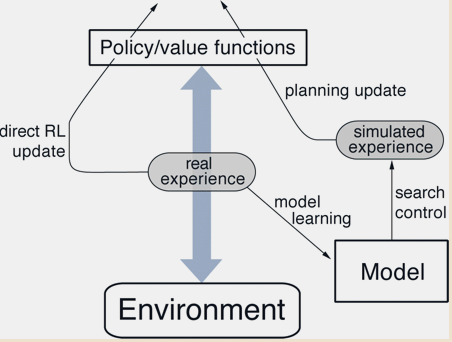
\includegraphics[width=.5\textwidth]{figures/dyna-architecture}
\end{center}
\caption{\
The general Dyna Architecture.\
Real experience, passing back and forth between the environment and the policy,\
affects policy and value functions in much the same way as does simulated experience generated by the model of the environment.\
}
\label{fig:dyna-architecture}
\end{figure}


\begin{table}
\beginalg
Initialize $Q(\curs,\cura)$ and $Model(\curs,\cura)$ for all $s\in\stateset$ and $\cura\in\actionset(S)$\\
\\
Loop:\\
\> $S \assign$ current (nonterminal) state\\
\> $A \assign$ \epsgreedy$(S,Q)$ \\
\> Take action $A$; observe reward $R$ and next state $S'$\\
\> Update Q-function: $Q(S,A) \assign (1-\alpha) Q(S,A) + \alpha \left( R + \df \max_{\cura\in\actionset(S)}Q(S',\cura)\right)$\\
\> $Model(S,A) \assign R, S'$ (assuming deterministic environment)\\
\> Loop repeat\\
\> Apply one-step tabular Q-learning to $S$, $A$, $R$, $S'$:\\
\> \> $S \assign$ random previously observed state\\
\> \> $A \assign$ random action previously taken in $S$\\
\> \> $R, S' \assign Model(S,A)$\\
\> \> Update Q-function: $Q(S,A) \assign (1-\alpha) Q(S,A) + \alpha \left( R + \df \max_{\cura\in\actionset(S)}Q(S',\cura) \right)$\\
Until a certain criterion is satisfied
\endalg
\caption{Tabular Dyna-Q}
\label{tab:alg:tabular-dyna-q}
\end{table}


\section{On-policy Prediction with Approximation}

XXX

\section{On-policy Control with Approximation}

XXX

\section{Off-policy Methods with Approximation}

XXX

\section{Eligibility Traces}



Eligibility traces are one of the basic mechanisms of reinforcement learning.
Almost any temporal-difference (TD) method,
such as Q-learning or Sarsa,
can be combined with eligibility traces to obtain a more general method that may learn more efficiently.

We have already seen one way of unifying TD and Monte Carlo methods:
the $n$-step TD methods \S\ref{sec:n-step}.
What eligibility traces offer beyond these is an elegant algorithmic mechanism
with significant computational advantages.

The mechanism is a short-term memory vector,
the \emph{eligibility trace} $\et{t} \in \reals^\wvectdim$
that parallels the long-term weight vector $\wvector{t} \in \reals^\wvectdim$.
The rough idea is that when a component of \wvector{t}\ participates in producing an estimated value,
then the corresponding component of \et{t}\ is bumped up and then begins to fade away.
Learning will then occur in that component of \wvector{t}\
if a nonzero TD error occurs before the trace falls back to zero.
The \emph{trace-decay parameter} $\tdparam\in[0,1]$
determines the rate at which the trace falls.

The primary computational advantage of eligibility traces over $n$-step methods
is that only a single trace vector is required
rather than a store of the last $n$ feature vectors.
Learning also occurs continually and uniformly in time
rather than being delayed and then catching up at the end of the episode.
In addition
learning can occur and affect behavior
immediately after a state is encountered rather than being delayed $n$ steps.


\subsection{The \tdparam-return}

In \S\ref{sec:n-step} we defined an $n$-step return
as the sum of the first $n$ rewards plus the estimated value of the state reached in $n$ steps,
each appropriately discounted.
The general form of that equation,
for any parameterized function approximator, is
\begin{equation}
\label{eq:nstep-return}
\nstepreturn{t}{t+n}
=
\reward{t+1} + \df \reward{t+2} + \df^2 \reward{t+3} + \cdots + \df^{n-1} \reward{t+n}
+ \df^n \valappr(\state{t+n}, \wvector{t+n-1})
\end{equation}

Now we note that a valid update can be done not just toward any $n$-step return,
but toward any average of $n$-step returns for different $n$s.
An example of such an average can be
the average of $3$-step return, $5$-step return, and $7$-step return,
\ie,
\begin{equation}
\frac{1}{3}(
\nstepreturn{t}{t+3}
+\nstepreturn{t}{t+5}
+\nstepreturn{t}{t+7}
)
\end{equation}

This is one example, but averaging produces a substantial new range of algorithms.
For example, we can average across many $n$-step returns
from $1$-step return to $\infty$-step return
to obtain another way of interrelating TD and Monte Carlo methods.
Nn principle, one could even average experience-based updates
with DP updates to get a simple combination of experience-based and model-based methods.

An update that averages simpler component updates is called a compound update.
The TD(\tdparam) algorithm can be understood as one particular way of averaging $n$-step updates.
This average contains all the $n$-step updates,
each weighted proportionally to $\tdparam^n$ (where $\tdparam\in[0,1]$),
and is normalized (to ensure that the weights sum to $1$).
The resulting update is toward a return, called the \tdparam-return , defined in its state-based form by

\begin{equation}
\label{eq:lambda-return}
\ldreturn{t} = (1-\tdparam) \sum_{n=1}^\infty \tdparam^{n-1} \nstepreturn{t}{t+n}
\end{equation}
where $(1-\tdparam) \sum_{n=1}^\infty \tdparam^{n-1} = 1$.
If the episode terminates at $t=T$,
then $\nstepreturn{t}{t+n} = \nstepreturn{t}{T} = \return{t}$ for all $n \geq T-t$,
thus,
\begin{equation}
\ldreturn{t} = (1-\tdparam) \sum_{n=1}^{T-t-1} \tdparam^{n-1} \nstepreturn{t}{t+n}
+ (1-\tdparam) \sum_{n=T-t}^\infty \tdparam^{n-1} \nstepreturn{t}{t+n}
= (1-\tdparam) \sum_{n=1}^{T-t-1} \tdparam^{n-1} \nstepreturn{t}{t+n}
+ \tdparam^{T-t-1} \return{t}.
\end{equation}

Note that if $\tdparam=1$, $\ldreturn{t}$ becomes the original return \return{t}.
Thus, updating value functions according to \tdparam-return is equivalent to Monte Carlo algorithm.
On the other hand, if $\tdparam=0$,
$\ldreturn{t}$ becomes $\nstepreturn{t}{t+1}$,
hence updating value functions according to \tdparam-return is equivalent to
the one-step temporal difference method,
\ie, TD($0$) method.

Now we define our first learning algorithm based on the \tdparam-return:
the \emph{off-line \tdparam-return algorithm}.
As an off-line algorithm,
it makes no changes to the weight vector during the episode.
Then, at the end of the episode,
a whole sequence of off-line updates are made according
to the semi-gradient method
using the \tdparam-return as the target.
The update rule of this method is
\begin{equation}
\label{eq:off-line-lambda-return-update}
\wvector{t+1} = \wvector{t}
+ \stepsize{t} \left( \ldreturn{t} - \valappr(\state{t}, \wvector{t})
\right) \nabla_{\wvector{}} \valappr(\state{t}, \wvector{t})
\end{equation}
for $t=0,\ldots, T-1$.
The \tdparam-return gives us
an alternative way of moving smoothly
between Monte Carlo and one-step TD methods
that can be compared with the $n$-step bootstrapping.

The above approach is what can be called the \emph{theoretical or forward} view of a learning algorithm.
For each state visited, we look forward in time to all the future rewards and decide how best to combine them.

\subsection{TD(\tdparam)}

TD(\tdparam) is one of the oldest and most widely used algorithms in reinforcement learning.
It was the first algorithm for which a formal relationship was shown between a more theoretical forward view
and a more computationally congenial backward view using eligibility traces.
Here we will show empirically that it approximates the off-line \tdparam-return algorithm
presented in the previous section.

TD(\tdparam) improves over the off-line \tdparam-return algorithm in three ways.
\begin{itemize}
\item It updates the weight vector on every step of an episode rather than only at the end,
thus its estimates is updated sooner (and may be better sooner).
\item Its computations are equally distributed in time
(rather than all at the end of the episode).
\item It can be applied to continuing problems rather than just to episodic problems.
\end{itemize}
The semi-gradient version of TD(\tdparam) with function approximation
will be shown below.

The \emph{eligibility trace} is a vector $\et{t} \in \reals^\wvectdim$
where the number of components of \et{t}\ is the same as that of \wvector{t}.
Whereas the \emph{weight vector}, \wvector{t}, is a long-term memory
accumulating over the lifetime of the system,
the eligibility trace is a short-term memory,
which typically lasts shorter than the length of an episode.
Eligibility traces assist in the learning process;
their only consequence is that they affect the weight vector,
and then the weight vector determines the estimated value.
At the same time, the eligibility traces plays a critical role
since that is what propagates future reward to the current one,
or equivalently, current reward back to the past states.

In TD(\tdparam),
the eligibility trace vector is initialized to zero at the beginning of the episode,
is incremented on each time step by the value gradient,
and then fades away by $\df \tdparam$
additively,
\ie,
\begin{eqnarray}
\nonumber
\et{t-1} &\assign& 0
\\
\et{t} &\assign& \df \tdparam \et{t-1} + \nabla_{\wvector{}} \valappr(\state{t}, \wvector{t}),
\ 0 \leq t \leq T
\label{eq:et:et-update}
\end{eqnarray}
where \df\ is the \emph{discount rate} and \tdparam\ is the \emph{trace-decay parameter}.

The eligibility trace keeps track of which components of the weight vector have contributed, positively or negatively,
to recent state valuations,
where ``recent'' is defined in terms of $\df \tdparam$.
The trace indicates the eligibility of each component of the weight vector for undergoing learning changes
should a reinforcing event occur where
the reinforcing events are the moment-by-moment one-step TD errors.
The TD error for state-value prediction is
\begin{equation}
\label{eq:et:td-error}
\tderror{t} \assign \reward{t+1} + \df \valappr(\state{t+1}, \wvector{t}) - \valappr(\state{t}, \wvector{t})
\end{equation}
Finally, the weight vector is updated on each step
proportionally to all three factors;
the step size,
the TD error,
and the eligibility trace,
\ie,
\begin{equation}
\label{eq:et:weight-vector-update}
\wvector{t+1} \assign \wvector{t} + \stepsize{t} \tderror{t} \et{t}.
\end{equation}

\tablename~\ref{tab:alg:et:semi-gradient} described the \emph{semi-gradient TD(\tdparam) algorithm} for estimating $\valappr \sim v_\pol$
using
(\ref{eq:et:et-update}),
(\ref{eq:et:td-error}),
and
(\ref{eq:et:weight-vector-update}).

\begin{table}
\beginalg
Inputs:\\
\> \pol\ to be evaluated
\\
\> differential function $\valappr: \nonterminalstateset \times \reals^\wvectdim \to \reals$
	such that $\valappr(\mathrm{terminal}, \cdot) = 0$
\\\\
Algorithm parameters:
\\
\> trace-decay parameter, $\tdparam \in [0,1]$, and step size, $\stepsize{t}>0$
\\\\
Initialize:
\\\\
\> Initialize value-function weights \wvector{}\ arbitrarily
\\\\
Loop for each episode:\\
\> Initialize \state\
\\
\> $\et{} \assign 0$
\\
\> Loop for each step of episode:
\\
\> \> Choose $\action{} \sim \pol(\cdot|\state{})$\\
\> \> Take action \action, observe \reward{}, $\state{}'$\\
%\> \> $\et{} \assign \df \tdparam \et{} + \nabla_{\wvector{}} \valappr(\state{}, \wvector{})$\\
\> \> $\tderror{} \assign \reward{} + \df \valappr(\state{}', \wvector{}) - \valappr(\state{}, \wvector{})$\\
\> \> $\wvector{} \assign \wvector{} + \stepsize{t} \tderror{} \et{}$\\
\> \> $\state{} \assign \state{}'$
\\
\> until $S'$ is terminal
\endalg
\caption{Semi-gradient TD(\tdparam) algorithm for estimating $\valappr \sim v_\pol$.}
\label{tab:alg:et:semi-gradient}
\end{table}


\subsection{Why TD(\tdparam) approximates the off-line \tdparam-return algorithm?}

Here we examine why TD(\tdparam) approximates the off-line \tdparam-return algorithm.

In this section, we drop the subscript $t$ from \wvector{t}.
Because of this, we can only prove thet TD(\tdparam) is \emph{approximately} the same as the off-line \tdparam-return algorithm.
In fact, they are different.

First, the $n$-step return at $t$ can be rewritten in terms of that at $t+1$ as follows.
\begin{eqnarray*}
\nstepreturn{t}{t+n}
&=& \reward{t+1} + \df \reward{t+2} + \df^2 \reward{t+3} + \cdots + \df^{n-1} \reward{t+n}
+ \df^n \valappr(\state{t+n}, \wvector{})
\\
&=& \reward{t+1} + \df \reward{t+2} + \df^2 \reward{t+3} + \cdots + \df^{n-1} \reward{t+n}
\\
&& + \df \valappr(\state{t+1}, \wvector{}) - \valappr(\state{t}, \wvector{})
\\
&& + \df(\df \valappr(\state{t+2}, \wvector{}) - \valappr(\state{t+1}, \wvector{}))
\\
&& + \cdots
\\
&& + \df^{n-1} (\df \valappr(\state{t+n}, \wvector{}) - \valappr(\state{t+n-1}, \wvector{}))
\\
&& + \valappr(\state{t}, \wvector{})
\\
&=& \reward{t+1} + \df \valappr(\state{t+1}, \wvector{}) - \valappr(\state{t}, \wvector{})
\\
&& + \df(\reward{t+2} + \df \valappr(\state{t+2}, \wvector{}) - \valappr(\state{t+1}, \wvector{}))
\\
&& + \cdots
\\
&& + \df^{n-1} (\reward{t+n} + \df \valappr(\state{t+n}, \wvector{}) - \valappr(\state{t+n-1}, \wvector{}))
\\
&& + \valappr(\state{t}, \wvector{}),
\end{eqnarray*}
thus, (\ref{eq:et:td-error}) implies
\begin{equation}
\label{eq:nusl}
\nstepreturn{t}{t+n}
= \tderror{t} + \df \tderror{t+1} +  \cdots + \df^{n-1} \tderror{t+n-1} + \valappr(\state{t}, \wvector{})
\end{equation}

\iffalse
\begin{eqnarray}
\nonumber
\nstepreturn{t}{t+n}
&=& \reward{t+1} + \df \reward{t+2} + \df^2 \reward{t+3} + \cdots + \df^{n-1} \reward{t+n}
+ \df^n \valappr(\state{t+n}, \wvector{})
\\
\nonumber
&=& \reward{t+1} + \df \reward{t+2} + \df^2 \reward{t+3} + \cdots + \df^{n-1} \reward{t+n}
+ \df^{n} \reward{t+n+1}
+ \df^{n+1} \valappr(\state{t+n+1}, \wvector{})
\\
\nonumber
&&
+ \df^n \valappr(\state{t+n}, \wvector{})
- \df^{n} \reward{t+n+1}
- \df^{n+1} \valappr(\state{t+n+1}, \wvector{})
\\
\nonumber
&=& \reward{t+1} + \df \left(\reward{t+2} + \df \reward{t+3} + \cdots + \df^{n-2} \reward{t+n}
+ \df^{n-1} \reward{t+n+1}
+ \df^{n} \valappr(\state{t+n+1}, \wvector{})
\right)
\\
\nonumber
&&
+ \df^n \valappr(\state{t+n}, \wvector{})
- \df^{n} \reward{t+n+1}
- \df^{n+1} \valappr(\state{t+n+1}, \wvector{})
\\
\nonumber
&=& \reward{t+1} + \df \nstepreturn{t+1}{t+n+1}
- \df^n \left( \reward{t+n+1} + \df \valappr(\state{t+n+1}, \wvector{}) - \valappr(\state{t+n}, \wvector{}) \right)
\\
&=& \reward{t+1} + \df \nstepreturn{t+1}{t+n+1} - \df^n \tderror{t+n}
\label{eq:difkc}
\end{eqnarray}
where
(\ref{eq:nstep-return}) and (\ref{eq:et:td-error}) are used.
\fi

Now (\ref{eq:nusl}) together with (\ref{eq:lambda-return}) implies that
\begin{eqnarray*}
\ldreturn{t} &=& (1-\tdparam) \sum_{n=1}^\infty \tdparam^{n-1} \nstepreturn{t}{t+n}
\\
&=& (1-\tdparam) \sum_{n=1}^\infty \tdparam^{n-1}
\left( \tderror{t} + \df \tderror{t+1} +  \cdots + \df^{n-1} \tderror{t+n-1} + \valappr(\state{t}, \wvector{}) \right)
\\
&=& (1-\tdparam) \sum_{n=1}^\infty \tdparam^{n-1}
\left(\sum_{k=0}^{n-1} \df^k \tderror{t+k} + \valappr(\state{t}, \wvector{}) \right)
\\
&=& (1-\tdparam) \sum_{n=1}^\infty \tdparam^{n-1}
\left(\sum_{k=0}^{n-1} \df^k \tderror{t+k} \right)
+ (1-\tdparam) \sum_{n=1}^\infty \tdparam^{n-1} \valappr(\state{t}, \wvector{})
\\
&=& (1-\tdparam) \sum_{n=1}^{\infty} \sum_{k=0}^{n-1} \tdparam^{n-1} \df^k \tderror{t+k}
+ (1-\tdparam) \sum_{n=1}^\infty \tdparam^{n-1} \valappr(\state{t}, \wvector{})
\\
&=& (1-\tdparam) \sum_{k=0}^{\infty} \sum_{n=k+1}^\infty \tdparam^{n-1} \df^k \tderror{t+k}
+ (1-\tdparam) \sum_{n=1}^\infty \tdparam^{n-1} \valappr(\state{t}, \wvector{})
\\
&=& (1-\tdparam) \sum_{k=0}^{\infty} \df^k \tderror{t+k} \sum_{n=k+1}^\infty \tdparam^{n-1}
+ \valappr(\state{t}, \wvector{})
\\
&=& \sum_{k=0}^{\infty} (\df \tdparam)^k \tderror{t+k} + \valappr(\state{t}, \wvector{})
\end{eqnarray*}
since $(1-\tdparam) \sum_{n=1}^\infty \tdparam^{n-1} = 1$,
thus
\begin{equation}
\ldreturn{t} - \valappr(\state{t}, \wvector{}) = \sum_{k=0}^{\infty} (\df \tdparam)^k \tderror{t+k}.
\end{equation}
If an episode ends at $t=T$, then \tderror{t}\ for $t\geq T$,
hence
\begin{equation}
\label{eq:bysig}
\ldreturn{t} - \valappr(\state{t}, \wvector{}) = \sum_{k=0}^{T-t-1} (\df \tdparam)^k \tderror{t+k}.
\end{equation}

Now we derived a formula for \et{t+n}\ using summation notation from the recursive formula (\ref{eq:et:et-update}).
\begin{eqnarray*}
\et{t+n} &=& \df \tdparam \et{t+n-1} + \nabla_{\wvector{}} \valappr(\state{t+n},\wvector{})
\\
&=& \df \tdparam \left(
\df \tdparam \et{t+n-2} + \nabla_{\wvector{}} \valappr(\state{t+n-1},\wvector{})
\right)
+ \nabla_{\wvector{}} \valappr(\state{t+n},\wvector{})
\\
&=& (\df \tdparam )^2 \et{t+n-2} + (\df \tdparam) \nabla_{\wvector{}} \valappr(\state{t+n-1},\wvector{})
+ \nabla_{\wvector{}} \valappr(\state{t+n},\wvector{})
\\
&\vdots&
\\
&=& (\df \tdparam )^{n} \nabla_{\wvector{}} \valappr(\state{t},\wvector{})
+ (\df \tdparam)^{n-1} \nabla_{\wvector{}} \valappr(\state{t+1},\wvector{})
%+ (\df \tdparam)^{n-2} \nabla_{\wvector{}} \valappr(\state{t+2},\wvector{})
+ \cdots
+ (\df \tdparam) \nabla_{\wvector{}} \valappr(\state{t+n-1},\wvector{})
+ \nabla_{\wvector{}} \valappr(\state{t+n},\wvector{}),
\end{eqnarray*}
thus,
\begin{equation}
\label{eq:vyduf}
\et{t+n} = \sum_{k=0}^n (\df \tdparam)^{n-k} \nabla_{\wvector{}} \valappr(\state{t+k},\wvector{}).
\end{equation}
We can prove (\ref{eq:vyduf}) mathematically strictly using the mathematical induction.

We also derive a formula for \wvector{t+n}\ using summation notation from the recursive formula (\ref{eq:et:weight-vector-update})
and (\ref{eq:et:td-error}).
\begin{eqnarray*}
\wvector{t+n} &=& \stepsize{} \tderror{t+n-1} \et{t+n-1} + \wvector{t+n-1}
\\
&=& \stepsize{} \left( \tderror{t+n-1} \et{t+n-1} + \tderror{t+n-2} \et{t+n-2} \right) + \wvector{t+n-2}
\\
&=& \stepsize{} \left(
\tderror{t+n-1} \et{t+n-1} + \tderror{t+n-2} \et{t+n-2} + \cdots + \tderror{t+1} \et{t+1} + \tderror{t} \et{t}
\right)
+ \wvector{t}
\end{eqnarray*}
where we drop the subscript from the step size \stepsize{t}.
Thus,
\begin{equation}
\label{eq:nuasdk}
\wvector{t+n} = \stepsize{} \sum_{j=0}^{n-1}  \tderror{t+j} \et{t+j} + \wvector{t}.
\end{equation}

Now combining (\ref{eq:vyduf}) and (\ref{eq:nuasdk}) yields
\begin{eqnarray*}
\wvector{t+n} - \wvector{t}
&=& \stepsize{} \sum_{j=0}^{n-1}  \tderror{t+j} \et{t+j}
\\
&=& \stepsize{} \sum_{j=0}^{n-1}  \tderror{t+j} 
\sum_{k=0}^j (\df \tdparam)^{j-k} \nabla_{\wvector{}} \valappr(\state{t+k},\wvector{}).
\\
&=& \stepsize{} \sum_{j=0}^{n-1} \sum_{k=0}^j (\df \tdparam)^{j-k}
\tderror{t+j} \nabla_{\wvector{}} \valappr(\state{t+k},\wvector{}).
\\
&=& \stepsize{} \sum_{k=0}^{n-1} \sum_{j=k}^{n-1} (\df \tdparam)^{j-k}
\tderror{t+j} \nabla_{\wvector{}} \valappr(\state{t+k},\wvector{})
\\
&=& \stepsize{} \sum_{k=0}^{n-1} \nabla_{\wvector{}} \valappr(\state{t+k},\wvector{})
\sum_{j=k}^{n-1} (\df \tdparam)^{j-k} \tderror{t+j}
\\
&=& \stepsize{} \sum_{k=0}^{n-1} \nabla_{\wvector{}} \valappr(\state{t+k},\wvector{})
\sum_{j=0}^{n-k-1} (\df \tdparam)^{j} \tderror{t+k+j}
\\
&=& \stepsize{} \sum_{k=0}^{n-1} \nabla_{\wvector{}} \valappr(\state{t+k},\wvector{})
\sum_{j=0}^{n+t-(t+k)-1} (\df \tdparam)^{j} \tderror{(t+k)+j}
\end{eqnarray*}
which together with (\ref{eq:bysig}) implies
\begin{eqnarray}
\nonumber
\wvector{T} - \wvector{t}
&=& \stepsize{} \sum_{k=0}^{T-t-1} \nabla_{\wvector{}} \valappr(\state{t+k},\wvector{})
\sum_{j=0}^{T-(t+k)-1} (\df \tdparam)^{j} \tderror{(t+k)+j}
\\
\nonumber
&=& \stepsize{} \sum_{k=0}^{T-t-1} \nabla_{\wvector{}} \valappr(\state{t+k},\wvector{})
\left( \ldreturn{t+k} - \valappr(\state{t+k}, \wvector{}) \right)
\\
\nonumber
&=& \stepsize{} \sum_{k=0}^{T-t-1}
\left( \ldreturn{t+k} - \valappr(\state{t+k}, \wvector{}) \right)
\nabla_{\wvector{}} \valappr(\state{t+k},\wvector{}).
\\
&=& \stepsize{} \sum_{k=t}^{T-1}
\left( \ldreturn{k} - \valappr(\state{k}, \wvector{}) \right)
\nabla_{\wvector{}} \valappr(\state{k},\wvector{}).
\label{eq:ishfg}
\end{eqnarray}

Now observer that the update rule for off-line \tdparam-return algorithm
(\ref{eq:off-line-lambda-return-update}) implies that
\begin{eqnarray}
\nonumber
\wvector{T}
&=& \stepsize{} \left( \ldreturn{T-1} - \valappr(\state{T-1}, \wvector{}) \right) \nabla_{\wvector{}} \valappr(\state{T-1}, \wvector{})
+ \wvector{T-1}
\\
\nonumber
&=&
\stepsize{} \left( \ldreturn{T-1} - \valappr(\state{T-1}, \wvector{}) \right) \nabla_{\wvector{}} \valappr(\state{T-1}, \wvector{})
+ \stepsize{} \left( \ldreturn{T-2} - \valappr(\state{T-2}, \wvector{}) \right) \nabla_{\wvector{}} \valappr(\state{T-2}, \wvector{})
+ \wvector{T-2}
\\
\nonumber
&\vdots&
\\
\nonumber
&=&
\stepsize{} \left( \ldreturn{T-1} - \valappr(\state{T-1}, \wvector{}) \right) \nabla_{\wvector{}} \valappr(\state{T-1}, \wvector{})
+ \cdots
+ \stepsize{} \left( \ldreturn{t} - \valappr(\state{t}, \wvector{}) \right) \nabla_{\wvector{}} \valappr(\state{t}, \wvector{})
+ \wvector{t}
\\
&=& \stepsize{} \sum_{k=t}^{T-1}
\left( \ldreturn{k} - \valappr(\state{k}, \wvector{}) \right)
\nabla_{\wvector{}} \valappr(\state{k},\wvector{})
+ \wvector{t}
\label{eq:gudif}
\end{eqnarray}
assuming that $\stepsize{t} = \stepsize{}$ and $\wvector{t}=\wvector{}$ for all $t$.
Comparing (\ref{eq:ishfg}) with (\ref{eq:gudif}) tells that
the off-line \tdparam-return algorithm and TD(\tdparam) are equivalent
when we drop $t$ from \wvector{t} and \stepsize{t}.
Therefore we have shown that TD(\tdparam) approximates the off-line \tdparam-return algorithm.



\newpage
\section{Appendix: conditional probability and expected value}
\label{sec:rl-app}


Suppose that we have a sequence of random variables, $X$, $Y$, and $Z$
with supports \suppx, \suppy, and \suppz.

Note that the definition of the conditional probability implies that
for all $x\in\suppx$, $y\in\suppy$, $z\in\suppz$ such that $p_Y(y)\neq0$ and $p_Z(z)\neq 0$,
\begin{equation}
\label{eq:vusg-1}
p_{X|Y}(x|y)
= \frac{p_{X,Y}(x,y)}{p_Y(y)}
\Leftrightarrow
p_{X,Y}(x,y) = p_{X|Y}(x|y) p_Y(y).
\end{equation}


\begin{equation}
\label{eq:vusg-2}
p(x,y|z)
= \frac{p(x,y,z)}{p(z)}
= \frac{p(x,y,z)}{p(y,z)} \frac{p(y,z)}{p(z)}
= p(x|y,z) p(y|z).
\end{equation}

Then (\ref{eq:vusg-1}) implies
\begin{eqnarray*}
\lefteqn{
\Expect(X)
= \int_\suppx x p_X(x) dx
}
\\
&=& \int_\suppx x \left(\int_\suppy p_{X,Y}(x,y) dy \right) dx
= \int_\suppx x \left(\int_\suppy p_{X|Y}(x|y)p_Y(y) dy \right) dx
\\
&=& \int_\suppy \int_\suppx x p_{X|Y}(x|y)p_Y(y) dx dy
= \int_\suppy \left( \int_\suppx x p_{X|Y}(x|y) dx \right) p_Y(y) dy
\\
&=& \int_\suppy \Expect (X|Y=y) p_Y(y) dy
= \Expect_Y \Expect_{X|Y} (X|Y),
\end{eqnarray*}
\begin{equation}
\Expect(X) = \Expect_{X|Y} (X|Y),
\end{equation}
and (\ref{eq:vusg-2}) implies
\begin{eqnarray*}
\lefteqn{
\Expect(X|Z=z)
= \int_\suppx x p_{X|Z}(x|z) dx
}
\\
&=& \int_\suppx x \left(\int_{\suppy} p_{X,Y|Z}(x,y|z) dy \right) dx
= \int_\suppx x \left(\int_{\suppy} p_{X|Y,Z}(x|y,z) p_{Y|Z}(y|z) dy \right) dx
\\
&=& \int_\suppy \int_\suppx x p_{X|Y,Z}(x|y,z) p_{Y|Z}(y|z) dx dy
= \int_\suppy \left( \int_\suppx x p_{X|Y,Z}(x|y,z) dx \right) p_{Y|Z}(y|z) dy
\\
&=& \int_\suppy \Expect(X|Y=y,Z=z) p_{Y|Z}(y|z) dy
= \Expect_{Y|Z=z} \Expect(X|Y,Z=z),
\end{eqnarray*}
\ie,
\begin{equation}
\label{eq:dkci}
\Expect(X|Z=z)
= \Expect_{Y|Z=z} \Expect(X|Y,Z=z).
\end{equation}



\iffalse
\appendix
\appendixpage
\addappheadtotoc


\chapter{Amazon Machine Learning University}

\section{Matrix Factorization and Dimension Reduction}


\subsection{Lecture}


\subsection{Assignments}

\subsubsection{Assignment \#2}

\paragraph{Question: Analyzing PCA [2pts]}


\#\#\#\# Compute SVD

\begin{enumerate}
\item We will compute the SVD of the adjusted image matrix, \verb+img_arr_adj+, $\bf{X}$. That is, we calculate the SVD as $\bf{X} = \bf{U} \bf{\Sigma}  \bf{V}^T$ where $\bf{U}$, $\bf{V}$ are left and right singlular vectors of $\bf{X}$ and $\bf{\Sigma}$ is the diagonal matrix of singular values. 
\item Interpret the components of SVD for the image matrix - What do $\bf{U}$, $\bf{\Sigma}$ and $\bf{V}$ represent? Which component corresponds to the eigenfaces (that is the fundamental building blocks to "re-construct" any image in the data set)?
\end{enumerate}




\paragraph{Answer for Analyzing PCA}

Let $m=32$ and $n=HW$, *i.e.*, $m$ is the number if images and $n$ is the number of pixles. Let $k$ be the rank of $X$. Note that $k\leq\min\{m, n\}$.

Suppose that $v_1, \ldots, v_k \in \reals^n$ be the column vectors of $V\in\reals^{n\times k}$,
that $u_1, \ldots, u_k \in \reals^m$ be the column vectors of $U\in\reals^{m\times k}$,
and that $\diag(\sigma_1,\ldots,\sigma_k)\in\reals^{k\times k}$ be the diagonal matrix with $k$ singular values as its diagonal entries.

Then we can express $X$ as
\begin{equation}
X = \sum_{j=1}^k \sigma_j u_j v_j^T \in\reals^{m\times n}.
\end{equation}
This means the whole image set can be reconstructed with rank $1$ matrices $u_i v_i^T$ with coefficients $\sigma_j$. Thus,

* **$\Sigma$ represents how much each such component contributes to the whole image set.**

Now the $i$th image can be retrieved by $e_i^T X$ where $e_i\in\reals^m$ is the $i$th unit vector whose entries are zeros except the $i$the entriy, which is $1$.
Since
\begin{equation}
e_i^T X = \sum_{j=1}^k \sigma_j e_i^Tu_j v_j^T
= \sum_{j=1}^k (U_{i,j} \sigma_j) v_j^T \in\reals^{1\times n},
\end{equation}
**the $i$th image is the linear combination of $v_j$s with coefficients, $U_{i,j} \sigma_j$**. Thus,

* **$V$ represents the eigenfaces with which we can reconstruct the orignal faces.**

* **$U$ represents how much each eigefaces should contribute to reconstruct each original faces.**





\paragraph{Optional Question: SVD and Regression [bonus +3pts]}

This question is more theoretical in nature and lets you see how SVD can be used as a tool to derive expressions for problems involving matrices - We discussed square root of the matrix as an example in the lecture!
Let $\bf{X}$ be the data matrix and we have the SVD for the matrix with components given as $\bf{U}$, $\bf{\Sigma}$ and $\bf{V}$. Let $\bf{b}$ be the data corresponding to the output of the regression and $\bf{\theta}$ be the parameters we wish to learn. You may assume the bias term is already accounted for. The closed form solution to $\bf{\theta}$ is given by:
$$
{\bf{\theta}} = \left({\bf{X}}^T {\bf{X}} \right)^{-1}{\bf{X}}^T {\bf{b}}
$$

\begin{enumerate}
\item Express $\bf{\theta}$ exclusively in terms of the components of the SVD of $\bf{X}$ (i.e. $\bf{\theta}$ should only depend directly on $\bf{U}$, $\bf{\Sigma}$, $\bf{V}$ and $\bf{b}$).
\item Assume we have an L2 regularizer term with regularization hyper-parameter $\lambda$. The new closed form looks as follows: ${\bf{\theta}} = \left({\bf{X}}^T {\bf{X}} + \lambda {\bf{I}}\right)^{-1}{\bf{X}}^T {\bf{b}}$. Again, express $\bf{\theta}$ exclusively in terms of the components of the SVD of $\bf{X}$
\item Suppose that $\bf{X}$ is under-determined so that $\bf{X} \bf{\theta} = \bf{b}$ has infinitely many solutions. One particular solution is ${\bf{\theta}} = {\bf{X}}^{+} {\bf{b}}$, where ${\bf{X}}^{+}$ is the \emph{pseudo-inverse} of ${\bf{X}}$. Can you think of a way to express the pseudo-inverse in terms of $\bf{U}$, $\bf{\Sigma}$, $\bf{V}$ ? \emph{Hint}: It has an expression similar to what you obtained for question 1 above.
\end{enumerate}







\paragraph{Answers to the Optional Question}

\iffalse
\begin{equation}
\newcommand{\reals}{\mathbf{R}}
\newcommand{\rank}{\mathbf{rank}}$
\newcommand{\diag}{\mathbf{diag}}
\newcommand{\range}{\mathcal{R}}
\end{equation}
\fi

%\begin{equation}
\newcommand{\V}{\hat{V}}
\newcommand{\U}{\hat{U}}
\newcommand{\Sig}{\hat{\Sigma}}
%\end{equation}

First, we assume that $X$ is a $m$-by-$n$ matrix with rank $k$, *i.e.*,
\begin{equation}
X\in\reals^{m\times n},\
\rank\ A = k.
\end{equation}
Since the rank of $X$ equals to the maximum number of linearly independent columns of $X$, or equivalently, the maximum number of linearly independent rows of $X$, we should have $k\leq\min\{m,n\}$.

We also assume that $X$ has the following singular value decomposition (SVD):
\begin{equation}
X = U \Sigma V^T
\end{equation}
where $U\in\reals^{m\times k}$, $V\in\reals^{n\times k}$, and $\Sigma \in \reals^{k \times k}$.
By definition the column vectors of $U$ are orthonormal, *i.e.*, $u_i^T u_j = \delta_{i,j}$ where $\delta_{i,j}$ is the Kronecker delta function, *i.e.*,
\begin{equation}
\delta_{i,j} = \left\{\begin{array}{ll}
1 & i=j\\
0 & i\neq j
\end{array}\right.
\end{equation}
Therefore, we have $U^TU = I_k$. 
Likewise, the column vectors of $V$ are also orthonormal, *i.e.*, $v_i^T v_j = \delta_{i,j}$, hence, $V^TV=I_k$.
Thus, we have
\begin{equation}
U^TU = V^TV = I_k.
\end{equation}

We also note that for two matrices, $A$ and $B$, we have 
\begin{equation}
(AB)^T = B^T A^T
\end{equation}
assuming that the matrix multiplication $AB$ can be defined.
If we apply this recursively, we have
\begin{equation}
(A_1 A_2 \cdots A_n)^{T} = A_n^{T}A_{n-1}^{T}\cdots A_1^{T}.
\end{equation}
assuming that the matrix multiplication $A_1 A_2 \cdots A_n$ can be defined.

We want to show similar results for matrix inverse,
*i.e.*,
for any two nonsingular matrices of the same size, $A$ and $B$, we have
\begin{equation}
(AB)^{-1} = B^{-1}A^{-1}
\end{equation}
since $B^{-1}A^{-1} AB = B^{-1} B = I$.
If we apply this recursively, we have,
for any $n$ nonsingular matrices of the same size, $A_1$, $A_2$, $\ldots$, $A_n$,
\begin{equation}
(A_1 A_2 \cdots A_n)^{-1} = A_n^{-1}A_{n-1}^{-1}\cdots A_1^{-1}.
\end{equation}

**We will use these assumptions and results in the following.**







\begin{enumerate}
\item Express $\bf{\theta}$ exclusively in terms of the components of the SVD of $\bf{X}$ (i.e. $\bf{\theta}$ should only depend directly on $\bf{U}$, $\bf{\Sigma}$, $\bf{V}$ and $\bf{b}$).

**Answer:** $\theta = (X^TX)^{-1} X^T b = V \Sigma^{-1} U^T b$.

\begin{solution}
\begin{enumerate}







\item

**Proof 1:** Since  $X = U \Sigma V^T$ is the SVD of $X$,
\begin{equation}
X^T = (U\Sigma V^T)^T = (V^T)^T (U\Sigma)^T = V \Sigma^T U^T = V \Sigma U^T,
\end{equation}
using the fact that the traspose of the transpose of a matrix is the original matrix itself,
thus,
\begin{equation}
X^TX
= (V \Sigma U^T) (U \Sigma V^T) 
= V \Sigma (U^T U) \Sigma V^T
= V \Sigma^2 V^T.
\end{equation}
Note that 
$V\in\reals^{n\times k}$,
$\Sigma^2\in\reals^{k\times k}$,
and
$V^T\in\reals^{k\times n}$ with $k\leq n$.

The problem implicitly implies this matrix, $X^TX$, is nonsingular. If $k < n$, then $X^TX$ becomes rank-deficient, i.e., $\rank(X^TX) = k < n$, hence cannot be nonsingular.
Therefore we should have $k=n$, thus $V$ should be a square matrix.
Since $V^T V=I$, we have
\begin{equation}
V^{-1} = V^T.
\end{equation}

Therefore
\begin{eqnarray*}
\theta
&=&
(V \Sigma^2 V^T)^{-1} (V \Sigma U^T) b
\\
&=&
((V^T)^{-1} \Sigma^{-2} V^{-1}) (V \Sigma U^T) b
\\
&=&
(V \Sigma^{-2} V^T )(V \Sigma U^T) b = V \Sigma^{-2} (V^TV) \Sigma U^T b
\\
&=&
V \Sigma^{-1} U^T b,
\end{eqnarray*}
hence the proof!









\item

**Proof 2:**

We can see this in another way. Note that $\theta = (X^TX)^{-1}X^Tb$ is the optimal solution of the following optimization problem:
\begin{equation}
\begin{array}{ll}
\mbox{minimize} & \|Xx - b\|_2
\end{array}
\end{equation}
which is equivalent to
\begin{equation}
\begin{array}{ll}
\mbox{minimize} & \|U\Sigma V^T x - b\|_2
\end{array}
\end{equation}
where the optimization variable is $x\in\reals^n$.
Now if we let $y = \Sigma V^T x$, then this problem is equivalent to
\begin{equation}
\begin{array}{ll}
\mbox{minimize} & \|U y - b\|_2
\\
\mbox{subject to} & y = \Sigma V^T x.
\end{array}
\end{equation}
Using the fact that for any $x,y\in\reals^n$,
$\|x+y\|_2^2 = (x+y)^T(x+y) = x^Tx + y^Ty + 2x^Ty = \|x\|_2^2 + \|y\|_2^2 + 2x^Ty$,
we can dervie
\begin{eqnarray*}
\|U y - b\|_2^2
&=&
\|U (y - U^Tb) + UU^Tb - b\|_2^2
\\ &=&
\|U (y - U^Tb)\|_2^2 + \|UU^Tb - b\|_2^2
+2 (y-U^Tb)^T U^T (UU^Tb - b)
\\ &=&
\|U (y - U^Tb)\|_2^2 + \|UU^Tb - b\|_2^2
+2 (y-U^Tb)^T (U^TUU^Tb - U^Tb)
\\ &=&
\|U (y - U^Tb)\|_2^2 + \|UU^Tb - b\|_2^2
+2 (y-U^Tb)^T (U^Tb - U^Tb)
\\ &=&
\|U (y - U^Tb)\|_2^2 + \|UU^Tb - b\|_2^2
\\
&\geq&
\|UU^Tb - b\|_2^2
\end{eqnarray*}
where the equality holds if and only if $U (y - U^Tb)=0$.
Since this implies that $U^T U(y-U^Tb) = y-U^Tb = 0$,
and vice versa, we conclude that $U (y - U^Tb)=0$ if and only if $y=U^Tb$.

Therefore $y^\ast = U^Tb$ is the (only) optimal solution attaining its optimal value.
Thus,
\begin{equation}
\theta = x^\ast = (\Sigma V^T)^{-1} y^\ast = ((V^T)^{-1} \Sigma^{-1}) U^T b = V \Sigma^{-1} U^T b,
\end{equation}
hence the proof!










\item 

**Proof 3**

Here we use the same optimization problem as above, but take advantage of the convexity and the differentiability of the objective function.
The objective function of the above optimization problem is $\|Uy-b\|_2$. This is a convex function, but not differential for $y$ such that $Uy-b=0$.
Hence, we consider minimizing $\|Uy-b\|_2^2$. Now this function is not only differentiable, but also convex.
Hence it achives its minimum where the gradient vanishes.
Since
\begin{equation}
\nabla_y \|Uy-b\|_2^2 = \nabla_y U^T(Uy-b),
\end{equation}
equating this to zero implies
\begin{equation}
U^T(Uy-b) = 0 \Leftrightarrow U^TUy - U^Tb = 0 \Leftrightarrow y - U^Tb=0,
\end{equation}
hence we have the same results as above. Going throught the same procedure leads us to conlude that
\begin{equation}
\theta = x^\ast = (\Sigma V^T)^{-1} y^\ast = ((V^T)^{-1} \Sigma^{-1}) U^T b = V \Sigma^{-1} U^T b.
\end{equation}


\end{enumerate}

\end{solution}




\item Assume we have an L2 regularizer term with regularization hyper-parameter $\lambda$. The new closed form looks as follows: ${\bf{\theta}} = \left({\bf{X}}^T {\bf{X}} + \lambda {\bf{I}}\right)^{-1}{\bf{X}}^T {\bf{b}}$. Again, express $\bf{\theta}$ exclusively in terms of the components of the SVD of $\bf{X}$.

**Answer:**
$\theta = V \diag \left(\sigma_1/(\sigma_1^2+\lambda), \sigma_2/(\sigma_2^2+\lambda), \ldots, \sigma_k/(\sigma_k^2+\lambda) \right) U^T b$.
We observe that this quantity converges to $V\Sigma^{-1}U^Tb$ as $\lambda$ goes to $0$, which makes a perfect sense!

\begin{solution}


**Proof:** Since we don't assume that $X^TX$ is nonsingluar for this problem,
$V^T$ is not necessarily equal to $V^{-1}$. Indeed, $V$ is not a square matrix in general.
Thus, we introduce **full** SVD here as follows.

Let $v_1, \ldots, v_k\in\reals^n$ be the $k$ column vectors of $V$. These vectors are orthonormal.
Suppose that there are $n-k$ more vectors $v_{k+1}, \ldots, v_n\in\reals^n$ so that all the $n$ vectors, $v_1, \ldots, v_n\in\reals^n$ are orthonormal.
(We can find these vectors by, *e.g.*, applying Gram-Schmidt procedure to $\begin{bmatrix}v_1&\cdots&v_k&I_n\end{bmatrix}$.)
Now let $\hat{V}\in\reals^{n\times n}$ be a matrix such that
\begin{equation}
\V = \begin{bmatrix}V&v_{k+1}&\cdots&v_n\end{bmatrix} \in\reals^{n\times n}.
\end{equation}
Likewise, we can find $m-k$ vectors $u_{k+1}, \ldots, u_m\in\reals^m$ so that all the $m$ vectors, $u_1, \ldots, u_m\in\reals^m$ are orthonormal.
Let $\hat{U}\in\reals^{m\times m}$ be a matrix such that
\begin{equation}
\U = \begin{bmatrix}U&u_{k+1}&\cdots&u_m\end{bmatrix} \in\reals^{m\times m}.
\end{equation}
Now $\V$ is a square matrix with $\V^T \V = I_n$, hence $\V^T = \V^{-1}$.
For the same reason, $\U^T = \U^{-1}$.

Now we define $\Sig\in\reals^{m\times n}$ such that
\begin{equation}
\Sig_{i,j} = \left\{\begin{array}{ll}
        \sigma_i & \mbox{if } i = j \leq k\\
        0 & \mbox{otherwise}.
\end{array}\right.
\end{equation}
Then we have
\begin{equation}
X = \U \Sig \V^T,
\end{equation}
which is called **full SVD** of $X$.
That is, the very same matrix $X$ can also be expressed with bigger matrices.

Then

\begin{eqnarray}
X^TX + \lambda I &=& \left(\U\Sig \V^T\right)^T\left(\U \Sig \V^T\right) + \lambda I
= \V \Sig^T \U^T \U \Sig \V^T + \lambda I
\\
&=& \V \Sig^T\Sig  \V^T + \lambda I
= \V \Sig^T\Sig  \V^T + \lambda \V \V^T
\\
&=& \V (\Sig^T\Sig  + \lambda I) \V^T
\end{eqnarray}
where we use the fact that $\V^T = \V^{-1}$.
Note that $\Sig$ is not a square diagonal matrix (anymore),
hence the equation gets a bit different.

Therefore
\begin{eqnarray}
\theta
&=& (X^TX + \lambda I)^{-1} X^T b
= \left(\V(\Sig^T\Sig + \lambda I)\V^T \right)^{-1} \V \Sig^T \U^T b
\\
&=&
\left( \V(\Sig^T\Sig + \lambda I)^{-1} \V^T \right) \V \Sig^T \U^T b
= \V \left(\Sig^T\Sig + \lambda I \right)^{-1} \left(\V^T \V \right) \Sig^T \U^T b
\\
&=&
\V \left(\Sig^T\Sig + \lambda I \right)^{-1} \Sig^T \U^T b
\\
&=&
\V
f(\Sigma, \lambda)
\U^T b
\end{eqnarray}
where
\begin{equation}
f(\Sigma, \lambda) =
\begin{bmatrix}
\sigma_1/(\sigma_1^2+\lambda) & 0                             & \cdots & 0                             & 0          & \cdots
\\
0                             & \sigma_2/(\sigma_2^2+\lambda) & \cdots & 0                             & 0          & \cdots
\\
\vdots                        & \vdots                        & \ddots & 0                             & 0          & \cdots
\\
0                             & 0                             & \cdots & \sigma_k/(\sigma_k^2+\lambda) & 0          & \cdots
\\
0                             & 0                             & \cdots & 0                             & 0          & \cdots
\\
\vdots                        & \vdots                        & \vdots & \vdots                        & \vdots     & \ddots
\end{bmatrix}
\in\reals^{n\times m}
\end{equation}
Since this matrix has zero entries everywhere except the first $k$-by-$k$ major submatrix,
the latter $n-k$ column vectors in $\V$ diminishes as well as the latter $m-k$ column vectors in $\U$.
Therefore we have
\begin{equation}
\theta = V \diag \left(\sigma_1/(\sigma_1^2+\lambda), \sigma_2/(\sigma_2^2+\lambda), \ldots, \sigma_k/(\sigma_k^2+\lambda) \right) U^T b
\end{equation}
where $\diag(d_1,\ldots,d_k)\in\reals^{k\times k}$ denotes a (square) diagonal matrix whose diagonal entries are $d_1, \ldots, d_k$ (in this order),
hence the proof!

\end{solution}




\item Suppose that $\bf{X}$ is under-determined so that $\bf{X} \bf{\theta} = \bf{b}$ has infinitely many solutions. One particular solution is ${\bf{\theta}} = {\bf{X}}^{+} {\bf{b}}$, where ${\bf{X}}^{+}$ is the \emph{pseudo-inverse} of ${\bf{X}}$. Can you think of a way to express the pseudo-inverse in terms of $\bf{U}$, $\bf{\Sigma}$, $\bf{V}$ ? \emph{Hint}: It has an expression similar to what you obtained for question 1 above.

**Answer:** One solution can be expressed as
\begin{equation}
\theta^\ast = V\Sigma^{-1}U^Tb,
\end{equation}
*i.e.*, it is the same as the least-squre case. However, note that in this case, it should be satisfied that $
b\in\range(U)$ and $n>k$ where $k=\rank(X)$ and $\range(U)$ denotes the range of $U$, hence $\range(U) = \{Ux|x\in\reals^k\}$. Note that if $X$ is full-rank, then
\begin{equation}
\theta^\ast = X^T(XX^T)^{-1} b.
\end{equation}
Indeed, this solution is the minimum-norm solution for $X\theta=b$,
*i.e.*, for any $\theta$ satisfying $X\theta = b$, $\|\theta\|_2 \geq \|\theta^\ast\|_2$. The proof is given below.

\begin{solution}
\begin{enumerate}
\item


**Proof 1:**

If $\theta$ satisfies $X\theta=b$, then $U\Sigma V^T \theta = b$, 
hence, $b$ should be in the rnage of $X$, *i.e.*, $b\in\range(U)$.
Also,
\begin{eqnarray*}
U\Sigma V^T \theta = b
&\Rightarrow&
U^T(U\Sigma V^T \theta) = U^Tb
\\
&\Leftrightarrow&
(U^TU)\Sigma V^T \theta = \Sigma V^T \theta = U^Tb
\\
&\Leftrightarrow&
V^T \theta = \Sigma^{-1} U^Tb.
\end{eqnarray*}

Now let $V_0 \in\reals^{n\times(n-k)}$ be a matrix whose columns vectors comprise a basis for the null space of $V^T$.
Since the range of $\begin{bmatrix} V & V_0 \end{bmatrix}\in\reals^{n\times n}$ is $\reals^n$,
any $\theta\in\reals^n$ can be expressed as $\theta = Vx + V_0y$ for some $x\in\reals^k$ and $y\in\reals^{n-k}$.
Thus,
\begin{equation}
V^T\theta = V^TV x + V^TV_0 y = x = \Sigma^{-1} U^Tb
\end{equation}
since the columns of $V_0$ are a basis of the null space of $V^T$.
Therefore
\begin{equation}
\theta =  V\Sigma^{-1}U^Tb + V_0y.
\end{equation}
Now we show the converse is true,
*i.e.*,
we show that this satisfies $X\theta = b$ for every $y\in\reals^{n-k}$.
\begin{eqnarray*}
X(V\Sigma^{-1}U^Tb + V_0y)
&=& U\Sigma V^T(V\Sigma^{-1}U^Tb + V_0y)
\\
&=& U\Sigma (V^TV)\Sigma^{-1}U^Tb + U\Sigma V^T V_0y
\\
&=& UU^Tb.
\end{eqnarray*}
Now since we assume that $b\in\range(U)$,
$b=Uz$ for some $z\in\reals^k$.
Hence,
\begin{equation}
UU^Tb =  UU^TUz = Uz = b,
\end{equation}
thus
\begin{equation}
X(V\Sigma^{-1}U^Tb + V_0y) = b
\end{equation}
for all $y\in\reals^{n-k}$.
Since we assume that $X\theta = b$ has infinitely many solutions,
$V^T$ should have non-zero null space.
Note that $V^T$ has non-zero null space if and only if $n>k$.

In summary, $X\theta = b$ has infinitely many solution if and only if

* $b\in\range(U)$

* $n > k = \rank(X)$,

and
\begin{equation}
\theta^\ast = V\Sigma^{-1}U^Tb
\end{equation}
is one such solution.

Now we show that $\theta^\ast$ has the smallest $2$-norm among such solutions.
Assume that $\theta$ satisfies $X\theta = b$.
Then $\theta =  \theta^\ast + V_0y$, hence
\begin{eqnarray*}
\|\theta\|_2^2
&=& \| \theta^\ast + V_0y \|_2^2
\\
&=& \| \theta^\ast\|_2^2 +\| V_0y \|_2^2 + 2 y^T V_0^T \theta^\ast
\\
&=& \| \theta^\ast\|_2^2 +\| V_0y \|_2^2 + 2 y^T V_0^T V\Sigma^{-1}U^Tb
\\
&=& \| \theta^\ast\|_2^2 +\| V_0y \|_2^2 \geq \|\theta^\ast\|_2^2,
\end{eqnarray*}
thus $\theta^\ast$ has the smallest $2$-norm.










\item

**Proof 2:**

There is another way to prove the above argument.
The smallest $2$-norm solution can be found by solving the following optimization problem:
\begin{equation}
\begin{array}{ll}
\mbox{minimize} & \|\theta\|_2^2
\\
\mbox{subject to} & X\theta = b
\end{array}
\end{equation}

The Lagrangian $L:\reals^n\times\reals^m \to \reals$ is defined by
\begin{equation}
L(\theta, \nu) = \theta^T\theta + 2\nu^T(b-X\theta).
\end{equation}

Thus, the KKT optimality conditions are

* $X\theta^\ast = b$.

* $\nabla_\theta L(\theta^\ast, \nu^\ast) = 2\theta^\ast - 2X^T \nu^\ast = 0$

where $\theta^\ast$ is the primal optimum and $\nu^\ast$ is the dual optimum.

Then $\theta^\ast = X^T \nu^\ast$, hence $XX^T \nu^\ast = b$.
Since
\begin{equation}
XX^T \nu^\ast = U\Sigma V^T V \Sigma U^T \nu^\ast = U\Sigma^2 U^T \nu^\ast = b
\Rightarrow
\Sigma^2 U^T \nu^\ast = U^T b
\Leftrightarrow
U^T \nu^\ast = \Sigma^{-2} U^T b.
\end{equation}
Therefore
\begin{equation}
\theta^\ast = X^T \nu^\ast = V \Sigma U^T \nu^\ast = V \Sigma \Sigma^{-2} U^T b = V \Sigma^{-1} U^T b,
\end{equation}
hence the proof!


\end{enumerate}
\end{solution}

\end{enumerate}


\fi

\end{document}
